%!TEX encoding = UTF-8 Unicode
\documentclass{lecturehandouts}

\setbeamertemplate{footline}[frame number]
\title[Föreläsningsanteckningar pgk, 2016]{Programmering, grundkurs \code{pgk}}
\subtitle{Föreläsningsanteckningar \code{pgk} (EDAA45)}
\author{Björn Regnell}
\institute{Datavetenskap, LTH}
\date{Lp1-2, HT 2016}
 
\setbeamerfont{section in toc}{size=\small}

\setbeamerfont{subsection in toc}{size=\footnotesize}

\begin{document}

%\renewcommand{\pause}{}


\newcommand{\Lecture}[2]{%
\section[Vecka #1: #2]{#2}%
\frame{\tableofcontents[currentsubsection,hideothersubsections,sections={#1}]}}

\frame{\titlepage}
\frame{
\begin{multicols}{2}
\tableofcontents[subsectionstyle=hide,sections={1-7}]

\columnbreak

\tableofcontents[subsectionstyle=hide,sections={8-13}]

\end{multicols}
}

\Lecture{1}{Introduktion}
%!TEX encoding = UTF-8 Unicode
%!TEX root = ../lect-week01.tex

%%%%%%%%%%%%%%%%%%%%%%%%%%%%%%%%%%%%%%
\Subsection{Om kursen}

%%%

\ifkompendium\else
\begin{Slide}{Nytt för i år}
\begin{itemize}
\item \Emph{Scala} införs som förstaspråk på Datateknikprogrammet.
\item Den \Emph{största förnyelsen} av den inledande programmeringskursen sedan vi införde Java 1997.
\item Allt kursmaterial är \Emph{öppen källkod}.
\item \Emph{Studentermedverkan} i kursutvecklingen.
\end{itemize}
\vspace{1em}\hskip1em\href{https://www.lth.se/nyheter-och-press/nyheter/visa-nyhet/article/scala-blir-foerstaspraak-paa-datateknikprogrammet/}{www.lth.se/nyheter-och-press/nyheter/visa-nyhet/article/\\\hskip1emscala-blir-foerstaspraak-paa-datateknikprogrammet/}
\end{Slide}
\fi

\begin{Slide}{Veckoöversikt}
\noindent\resizebox{0.9\columnwidth}{!}{
%!TEX encoding = UTF-8 Unicode
\begin{tabular}{l|l|l|l}
\textit{W} & \textit{Modul} & \textit{Övn} & \textit{Lab} \\ \hline \hline
W01 & Introduktion            & expressions & kojo            \\
W02 & Kodstrukturer           & programs    & --              \\
W03 & Funktioner, Objekt      & functions   & bugs            \\
W04 & Datastrukturer          & data        & pirates         \\
W05 & Sekvensalgoritmer       & sequences   & cards           \\
W06 & Klasser, Likhet         & classes     & turtlegraphics  \\
W07 & Arv, Gränssnitt         & traits      & turtlerace-team \\
KS  & KONTROLLSKRIVN.         & --          & --              \\
W08 & Mönster, Undantag       & matching    & chords-team     \\
W09 & Matriser, Typparametrar & matrices    & maze            \\
W10 & Sökning, Sortering      & sorting     & surveydata-team \\
W11 & Scala och Java          & scalajava   & lthopoly-team   \\
W12 & Trådar                  & threads     & life            \\
W13 & Design                  & Uppsamling  & Projekt         \\
W14 & Tentaträning            & Extenta     & --              \\
T   & TENTAMEN                & --          & --              \\
\end{tabular}

}
\end{Slide}

\ifkompendium
\noindent Kursen består av en \textbf{modul} per läsvecka med två \textbf{föreläsningar}, en \textbf{övning} och en \textbf{laboration} (undantaget W02, W13 \& W14 som saknar labb och/eller övning). 
Föreläsningarna ger en översikt av den teori som ingår i varje modul. Genom att göra övningarna bearbetar du teorin och förebereder dig inför laborationerna. När du klarat övningen och laborationen i en modul är du redo att gå vidare till nästa. Tabellen på nästa uppslag visar begrepp som ingår i varje modul. 

Kursen är uppdelad i två läsperioder. Efter första läsperioden gör du en diagnostisk \textbf{kontrollskrivning} som kontrollerar ditt kunskapsläge. Andra läsperioden avslutas med ett större \textbf{projekt} och en skriftlig \textbf{tentamen}.



\clearpage
\hyphenation{intro-duktion sekvens-algoritmer kod-strukturer data-strukturer}
{\fontsize{11}{13}\selectfont\renewcommand{\arraystretch}{1.75}
\begin{longtable}{@{}p{.05\textwidth} | >{\hspace{0.1em}\raggedright\bfseries\sffamily}p{.15\textwidth}  >{\raggedleft\arraybackslash\hspace{0.0em}\fontsize{10.5}{12}\selectfont}p{0.735\textwidth}}
W01 & Introduktion & sekvens, alternativ, repetition, abstraktion, programmeringsspråk, programmeringsparadigmer, editera-kompilera-exekvera, datorns delar, virtuell maskin, REPL, literal, värde, uttryck, identifierare, variabel, typ, tilldelning, namn, val, var, def, inbyggda typer, Int, Long, Short, Double, Float, Byte, Char, String, println, typen Unit, enhetsvärdet (), stränginterpolatorn s, if, else, true, false, MinValue, MaxValue, aritmetik, slumptal, math.random, logiska uttryck, de Morgans lagar, while-sats, for-sats \\
W02 & Kodstrukturer & iterering, for-uttryck, map, foreach, Range, Array, Vector, algoritm vs implementation, pseudokod, algoritm: SWAP, algoritm: SUM, algoritm: MIN/MAX, algoritm: MININDEX, block, namnsynlighet, namnöverskuggning, lokala variabler, paket, import, filstruktur, jar, dokumentation, programlayout, JDK, main i Java vs Scala, java.lang.System.out.println \\
W03 & Funktioner, objekt & definera funktion, anropa funktion, parameter, returtyp, värdeandrop, namnanrop, default-argument, namngivna argument, applicera funktion på alla element i en samling, procedur, värdeanrop vs namnanrop, uppdelad parameterlista, skapa egen kontrollstruktur, objekt, modul, punktnotation, tillstånd, metod, medlem, funktionsvärde, funktionstyp, äkta funktion, stegad funktion, apply, lazy val, lokala funktioner, anonyma funktioner, lambda, aktiveringspost, anropsstacken, objektheapen, rekursion  cslib.window.SimpleWindow \\
W04 & Datastrukturer & attribut (fält), medlem, metod, tupel, klass, Any, isInstanceOf, toString, case-klass, samling, scala.collection, föränderlighet vs oföränderlighet, List, Vector, Set, Map, typparameter, generisk samling som parameter, översikt samlingsmetoder, översikt strängmetoder, läsa/skriva textfiler, Source.fromFile, java.nio.file \\
W05 & Sekvensalgoritmer & sekvensalgoritm, algoritm: SEQ-COPY, in-place vs copy, algoritm: SEQ-REVERSE, algoritm: SEQ-REGISTER, sekvenser i Java vs Scala, for-sats i Java, java.util.Scanner, scala.collection.mutable.ArrayBuffer, StringBuilder, java.util.Random, slumptalsfrö \\
W06 & Klasser & objektorientering, klass, Point, Square, Complex, new, null, this, inkapsling, accessregler, private, private[this], kompanjonsobjekt, getters och setters, klassparameter, primär konstruktor, objektfabriksmetod, överlagring av metoder, referenslikhet vs strukturlikhet, eq vs == \\
W07 & Arv & arv, polymorfism, trait, extends, asInstanceOf, with, inmixning, supertyp, subtyp, bastyp, override, klasshierarkin i Scala: Any AnyRef Object AnyVal Null Nothing, referenstyper vs värdetyper, klasshierarkin i scala.collection, Shape som bastyp till Point och Rectangle, accessregler vid arv, protected, final, klass vs trait, abstract class, case-object, typer med uppräknade värden \\
KS & \multicolumn{2}{l}{KONTROLLSKRIVN.} \\
W08 & Mönster, undantag & mönstermatchning, match, Option, throw, try, catch, Try, unapply, sealed, flatten, flatMap, partiella funktioner, collect, speciella matchningar: wildcard pattern; variable binding; sequence wildcard; back-ticks, equals, hashcode, exempel: equals för klassen Complex, switch-sats i Java \\
W09 & Matriser, typparametrar & matris, nästlad samling, nästlad for-sats, typparameter, generisk funktion, generisk klass, fri vs bunden typparameter, matriser i Java vs Scala, allokering av nästlade arrayer i Scala och Java \\
W10 & Sökning, sortering & strängjämförelse, compareTo, imlicit ordning, linjärsökning, binärsökning, algoritm: LINEAR-SEARCH, algortim: BINARY-SEARCH, algoritmisk komplexitet, sortering till ny vektor, sortering på plats, insättningssortering, urvalssortering, algoritm: INSERTION-SORT, algoritm: SELECTION-SORT, Ordering[T], Ordered[T], Comparator[T], Comparable[T] \\
W11 & Scala och Java & översikt av syntaxskillnader mellan Scala och Java, klasser i Scala vs Java, referensvariabler vs enkla värden i Java, referenstilldelning vs värdetilldelning i Java, alternativ konstruktor i Scala och Java, for-sats i Java, java for-each i Java, java.util.ArrayList, autoboxing i Java, primitiva typer i Java, wrapperklasser i Java, samlingar i Java vs Scala, scala.collection.JavaConverters, namnkonventioner för konstanter \\
W12 & Webb, trådar & översikt webbprogrammering, kort om html+css+javascript+scala.js, tråd, jämlöpande exekvering, icke-blockerande anrop, callback, java.lang.Thread, java.util.concurrent.atomic.AtomicInteger, scala.concurrent.Future \\
W13 & Design, api & utvecklingsprocessen, krav-design-implementation-test, gränssnitt, trait vs interface, programmeringsgränssnitt (api), designexempel \\
W14 & \multicolumn{2}{l}{Tentaträning} \\
T & \multicolumn{2}{l}{TENTAMEN} \\
\end{longtable}
}
\fi

\begin{Slide}{Vad lär du dig?}
\begin{itemize}
\item Grundläggande principer för programmering:\\ Sekvens, Alternativ, Repetition, Abstraktion (SARA)\\$\implies$Inga förkunskaper i programmering krävs!
\item Konstruktion av algoritmer
\item Tänka i abstraktioner
\item Förståelse för flera olika angreppssätt: 
\begin{itemize}
\item \Emph{imperativ programmering}%: satser, föränderlighet
\item \Emph{objektorientering}%: inkapsling, återanvändning
\item \Emph{funktionsprogrammering}%: uttryck, oföränderlighet
\end{itemize}
\item Programspråken \Emph{Scala} och \Emph{Java}
\item Utvecklingsverktyg (editor, kompilator, utvecklingsmiljö)
\item Implementera, testa, felsöka
\end{itemize}
\end{Slide}

\begin{Slide}{Hur lär du dig?}
\begin{itemize}
\item Genom praktiskt \Alert{eget arbete}: \Emph{Lära genom att göra!}
\begin{itemize}
\item Övningar: applicera koncept på olika sätt
\item Laborationer: kombinera flera koncept till en helhet
\end{itemize}
\item Genom studier av kursens teori: \Emph{Skapa förståelse!}
\item Genom samarbete med dina kurskamrater: \Emph{Gå djupare!}
\end{itemize}
\end{Slide}


\begin{Slide}{Kurslitteratur}
\begin{minipage}{0.45\textwidth}\SlideFontSmall
\hskip1.33em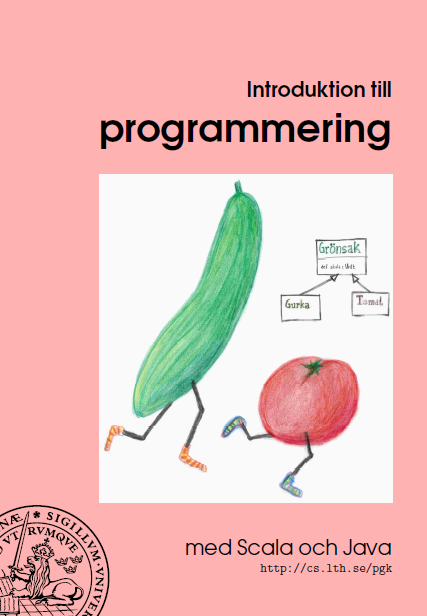
\includegraphics[width=0.65\textwidth]{../img/compendium-front-page.png}
\begin{itemize}
\item \Emph{Kompendium} med övningar \& laborationer, trycks \& säljs av inst. på beställning
\item Föreläsningsbilder
\item Nätresurser enl. länkar

\end{itemize}
\end{minipage}
\hskip1em\begin{minipage}{0.5\textwidth}\SlideFontSize{8}{10}
Bra, men ej nödvändig, \Emph{bredvidläsning}:\\ 
-- för \Emph{nybörjare}:
\vskip0.2mm
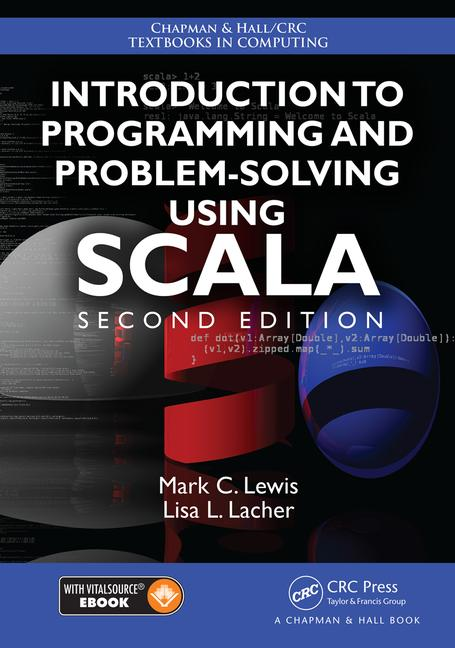
\includegraphics[width=0.33\textwidth]{../img/lewisbook.jpg}\hskip4mm
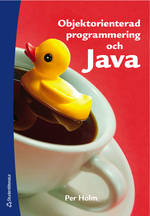
\includegraphics[width=0.33\textwidth]{../img/ankbok.jpg}

\noindent -- för de som \Emph{redan kodat} en del:
\vskip0.7mm
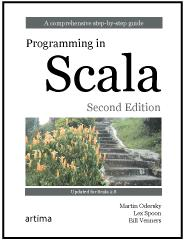
\includegraphics[width=0.45\textwidth]{../img/pinsbook.jpg}\hskip4mm
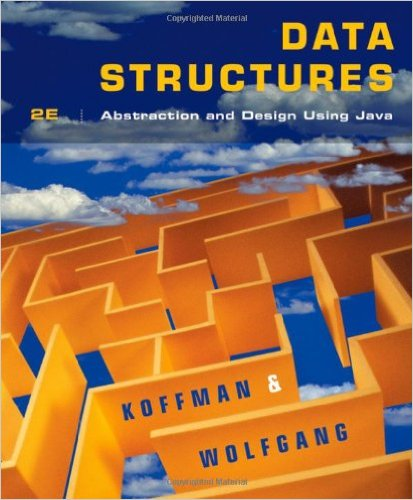
\includegraphics[width=0.47\textwidth]{../img/koffmanbook.jpg}
\end{minipage}
\end{Slide}

\ifkompendium
\noindent Kompendiet är den huvudsakliga kurslitteraturen och definierar kursinnehållet. Föreläsningar, övningar och laborationer i kompendiet är kursens primära kunskapskällor, tillsammans med de öppna resurser på nätet som kompendiet hänvisar till. Kompendiet är öppen källkod och du välkomnas varmt att bidra!

Om du gärna vill ha en eller flera mer traditionella läroböcker som bredvidläsning rekommenderas följande:
\begin{itemize}[noitemsep, leftmargin=*]
\item För de som aldrig kodat, och vill läsa om kodning från grunden:
\begin{itemize}[nolistsep]
\item ''Introduction to Programming and Problem-Solving Using Scala, Second Edition'', Mark C. Lewis, Lisa Lacher.  {\href{https://www.crcpress.com/Introduction-to-Programming-and-Problem-Solving-Using-Scala-Second-Edition/Lewis-Lacher/p/book/9781498730952}{www.crcpress.com/Introduction-to-Programming-and-Problem-Solving-Using-Scala-Second-Edition/Lewis-Lacher/p/book/9781498730952}}
\item ''Objektorienterad programmering och Java'', Per Holm, Tredje upplagan (2007). \href{https://www.studentlitteratur.se/#6735}{www.studentlitteratur.se/\#6735}
\end{itemize}
\item För de som redan kodat en hel del i ett objektorienterat språk:
\begin{itemize}[nolistsep, noitemsep]
\item ''Programming in Scala, Third Edition -- A comprehensive step-by-step guide'', Martin Odersky, Lex Spoon, and Bill Venners. \\ \href{http://www.artima.com/shop/programming_in_scala_3ed}{www.artima.com/shop/programming\_in\_scala\_3ed} 
\item ''Data Structures: Abstraction and Design Using Java, 3rd Edition'', Elliot B. Koffman, Paul A. T. Wolfgang. \\
\href{http://eu.wiley.com/WileyCDA/WileyTitle/productCd-1119186528.html}{http://eu.wiley.com/WileyCDA/WileyTitle/productCd-1119186528.html}
\end{itemize}
\end{itemize}
Dessa läroböcker följer inte direkt kursens upplägg vad gäller omfång och progression och du får själv göra den nyttiga hemläxan att koppla  deras innehåll till det vi går igenom i kursens olika moduler.

\else
\begin{Slide}{Beställning av kompendium och snabbreferens}\SlideFontSmall
\begin{itemize}
\item \Emph{Kompendiet} finns i pdf för fri nedladdning enl. CC-BY-SA, men det \Alert{rekommenderas starkt} att du köper den tryckta bokversionen.
\item Det är mycket lättare att ha övningar och labbar \Alert{på papper} \Emph{bredvid skärmen}, när du ska tänka, koda och plugga!
\item \Emph{Snabbreferensen} finns också i pdf men du behöver ha en tryckt version eftersom det är \Alert{enda tillåtna hjälpmedlet} på skriftliga kontrollskrivningen och tentamen.
\item Kompendiet och snabbreferens trycks här i E-huset och säljs av institutionen till självkostnadspris. Pris för kompendium+snabbreferens \Alert{beror på hur många som beställer}.
\item Snabbreferens enbart kostar 10 kr.
\item Skriv upp dig på listan -- tryckning sker efter beställning.
\item Du betalar \Alert{kontant} med \Emph{jämna pengar} på cs expedition, våning 2.
\end{itemize}
\end{Slide}
\fi

\ifkompendium\else
\begin{Slide}{Personal}\SlideFontSmall
\begin{description}
\item [\bfseries Kursansvarig:] ~\\Björn Regnell, bjorn.regnell@cs.lth.se
\item [\bfseries Kurssekreterare:]  ~\\Lena Ohlsson \\Exp.tid 09.30 -- 11.30 samt 12.45 -- 13.30
\item [\bfseries Handledare:] ~\\
\Emph{Doktorander}: \\ 
Tekn. Lic. Maj Stenmark, Gustav Cedersjö\\
\Emph{Teknologer}: \\
Anders Buhl, 
Anna Palmqvist Sjövall, 
Anton Andersson,
Cecilia Lindskog, 
Emil Wihlander, 
Erik Bjäreholt, 
Erik Grampp, 
Filip Stjernström, 
Fredrik Danebjer, 
Henrik Olsson, 
Jakob Hök, 
Jonas Danebjer, 
Måns Magnusson, 
Oscar Sigurdsson, 
Oskar Berg, 
Oskar Widmark, 
Sebastian Hegardt, 
Stefan Jonsson, 
Tom Postema, 
Valthor Halldorsson
\end{description}
\end{Slide}
\fi

\begin{Slide}{Föreläsningsanteckningar}
\begin{itemize}
\item Föreläsningsanteckningar utvecklas under kursens gång
\item Några av bilderna finns i kompendiet
\item Alla bilder läggs ut här: \\
\href{https://github.com/lunduniversity/introprog/tree/master/slides}{github.com/lunduniversity/introprog/tree/master/slides} \\
och uppdateras kontinuerligt allt eftersom de utvecklas
\item Förslag på förbättringar välkomna!
\end{itemize}
\end{Slide}

\begin{Slide}{Kursmoment --- varför?}\SlideOnly{\footnotesize}
\begin{itemize}
\item \Emph{Föreläsningar}: skapa översikt, ge struktur, förklara teori, svara på frågor, motivera varför
\item \Emph{Övningar}: \Alert{förbereda} laborationerna, bearbeta teorins olika delar med avgränsade deluppgifter, \Emph{grundövningar} för alla, \Emph{extraövningar} om du vill/behöver öva mer, \Emph{fördjupningsövningar} om du vill gå djupare 
\item \Emph{Laborationer}: \Alert{obligatoriska}, sätta samman teorins delar i ett större program; lösningar redovisas för handledare; gk på alla för att få tenta, 
\item \Emph{Resurstider}: få hjälp med övningar och laborationsförberedelser av handledare, fråga vad du vill
\item \Emph{Samarbetsgrupper}: grupplärande genom samarbete, hjälpa varandra 
\item \Emph{Kontrollskrivning}: \Alert{obligatorisk}, diagnostisk, kamraträttad; kan ge samarbetsbonuspoäng till tentan
\item \Emph{Individuell projektuppgift}: \Alert{obligatorisk}, du visar att du kan skapa ett större program självständigt; redovisas för handledare
\item \Emph{Tentamen}: \Alert{obligatorisk}, skriftlig, enda hjälpmedel: snabbreferensen\\   \url{http://cs.lth.se/pgk/quickref}
\end{itemize}
\end{Slide}

\ifkompendium\else
\begin{Slide}{Detta är bara början... }
Exempel på efterföljande kurser som bygger vidare på denna:
\begin{itemize}
\item Årskurs 1
\begin{itemize}
\item Programmeringsteknik -- fördjupningskurs
\item Utvärdering av programvarusystem
\item Diskreta strukturer
\end{itemize}
\item Årskurs 2
\begin{itemize}
\item Objektorienterad modellering och design
\item Programvaruutveckling i grupp
\item Algoritmer, datastrukturer och komplexitet
\item Funktionsprogrammering
\end{itemize}
\end{itemize}
\end{Slide}


\begin{Slide}{Registrering}
\begin{itemize}
\item Fyll i listan som skickas runt.
\item Kryssa i kolumnen \Emph{Ska gå} om du ska gå kursen\footnote{\scriptsize D1:a som redan gått motsvarande högskolekurs? Uppsök studievägledningen}\footnote{\scriptsize D2:a eller äldre som vill bli omregistrerad? Prata med kursansvarig på rasten}
\item Kryssa i kolumnen \Emph{Kursombud} om du kan tänka dig att vara kursombud under kursens gång
\begin{itemize}
\item Alla LTH-kurser ska utvärderas under kursens gång och efter kursens slut.
\item Till det behövs kursombud -- ungefär 2 D-are och 2 W-are.
\item Ni kommer att bli kontaktade av studierådet. \\SRD ordf: Amelia Andersson
\end{itemize}
\end{itemize}
\end{Slide}

%%%
\begin{Slide}{Förkunskaper}
\begin{itemize}
\item Förkunskaper $\neq$ Förmåga
\item Varken kompetens eller personliga egenskaper är statiska 
\item ''Programmeringskompetens'' är inte \textit{en} enda enkel förmåga utan en komplex sammansättning av flera olika förmågor som utvecklas genom hela livet
\item Ett innovativt utvecklar\Alert{team} behöver många olika kompetenser för att vara framgångsrikt
\end{itemize}
\end{Slide}

%%%
\begin{Slide}{Förkunskapsenkät}
\begin{itemize}
\item Om du inte redan gjort det fyll i förkunskapsenkäten \Alert{snarast}:
\url{http://cs.lth.se/pgk/survey} 
\item Dina svar behandlas internt och all redovisad statistik anonymiseras.
\item Enkäten ligger till grund för randomiserad gruppindelning i samarbetsgrupper, så att det blir en spridning av förkunskaper inom gruppen.
\item Gruppindelnig publiceras här: \\ \url{http://cs.lth.se/pgk/grupper/}
\end{itemize}
\end{Slide}

\begin{Slide}{Samarbetgrupper}\footnotesize
\begin{itemize}
\item Ni delas in i \Emph{samarbetsgrupper} om ca 5 personer baserat på förkunskapsenkäten, så att olika förkunskapsnivåer sammanförs
\item Några av laborationerna är mer omfattande \Emph{grupplabbar} och kommer att göras i samarbetsgrupperna \\ \vspace{1em}
\item Kontrollskrivningen i halvtid kan ge \Emph{samarbetsbonus} (max 5p) som adderas till ordinarie tentans poäng (max 100p) med medelvärdet av gruppmedlemmarnas individuella kontrollskrivningspoäng 
\scriptsize \parbox{7cm}{Bonus $b$ för varje person i en grupp med $n$ medlemmar med $p_i$ poäng vardera på kontrollskrivningen:} 
 \hspace{5mm} $\displaystyle b = \sum\limits_{i=1}^n \frac{p_i}{n}$
\end{itemize}
\end{Slide}

\fi

%%%
\begin{Slide}{Varför studera i samarbetsgrupper?}

Huvudsyfte: \Emph{Bra lärande!}

\begin{itemize}
\item Pedagogisk forskning stödjer tesen att lärandet blir mer djupinriktat om det sker i utbyte med andra
\item Ett studiesammanhang med höga ambitioner och respektfull gemenskap gör att vi \Emph{når mycket längre}
\item Varför ska du som redan kan mycket aktivt dela med dig av dina kunskaper?
\begin{itemize}
\item Förstå bättre själv genom att förklara för andra
\item Träna din pedagogiska förmåga
\item Förbered dig för ditt kommande yrkesliv som mjukvaruutvecklare 
\end{itemize}
\end{itemize}
\end{Slide}

%%%

\ifkompendium\else
\begin{Slide}{Samarbetskontrakt}
Gör ett skriftligt \href{https://github.com/bjornregnell/lth-eda016-2015/blob/master/assignments/collaboration-contract.tex}{\bf samarbetskontrakt} med dessa och ev. andra punkter som ni också tycker bör ingå:
\begin{enumerate}
\item Återkommande mötestider per vecka
\item Kom i tid till gruppmöten
\item Var väl förberedd genom självstudier inför gruppmöten
\item Hjälp varandra att förstå, men ta inte över och lös allt
\item Ha ett respektfullt bemötande även om ni har olika åsikter
\item Inkludera alla i gemenskapen
\end{enumerate}

Diskutera hur ni ska uppfylla dessa innan alla skriver på. \\ Ta med samarbetskontraktet och visa för handledare på labb 1.

\vskip1em

\Alert{Om arbetet i samarbetsgruppen inte fungerar ska ni mejla kursansvarig och boka mötestid!}
\end{Slide}

\begin{Slide}{Bestraffa inte frågor!}
\begin{itemize}
\item Det finns bättre och sämre frågor vad gäller hur mycket man kan lära sig av svaret, men \Emph{all undran är en chans} att i dialog utbyta erfarenheter och lärande
\item Den som frågar \Emph{vill veta} och berättar genom frågan något om nuvarande kunskapsläge
\item Den som svarar får chansen att \Emph{reflektera} över vad som kan vara svårt och olika vägar till djupare förståelse
\item I en hälsosam lärandemiljö är det \Emph{helt tryggt} att visa att man ännu inte förstår, att man gjort ''fel'', att man har mer att lära, etc. 
\item Det är viktigt att våga försöka även om det blir ''fel'':\\ \Emph{det är ju då man lär sig!}
\end{itemize}
\end{Slide}

%%%
\begin{Slide}{Plagiatregler}
Läs dessa regler noga och diskutera i samarbetsgrupperna:
\begin{itemize}
\footnotesize
\item \url{http://cs.lth.se/utbildning/samarbete-eller-fusk/}
\item \url{http://cs.lth.se/utbildning/foereskrifter-angaaende-obligatoriska-moment/}
\end{itemize}
Ni ska lära er genom \Emph{eget arbete} och genom  \Emph{bra samarbete}. Samarbete gör att man lär sig bättre, men man lär sig inte av att bara kopiera andras lösningar. Plagiering är förbjuden och kan medföra disciplinärende och avstängning.
\end{Slide}

\fi %%%%%%%%%%%%%%%%%%%%%%%%%%%%%%%%

%%%
\begin{Slide}{En typisk kursvecka}
\begin{enumerate}
\item Gå på \Emph{föreläsningar} på \Alert{måndag--tisdag}
\item Jobba med \Emph{individuellt} med teori, övningar, labbförberedelser på  \Alert{måndag--torsdag}
\item Kom till \Emph{resurstiderna} och få hjälp och tips av handledare och kurskamrater på \Alert{onsdag--torsdag}
\item Genomför den obligatoriska \Emph{laborationen} på \Alert{fredag}
\item Träffas i \Emph{samarbetsgruppen} och hjälp varandra att förstå mer och fördjupa lärandet, förslagsvis på återkommande tider varje vecka då alla i gruppen kan
\end{enumerate}
Se detaljerna och undantagen i schemat: \href{http://cs.lth.se/pgk/schema}{cs.lth.se/pgk/schema}
\end{Slide}

\ifkompendium\else  %%%%%%%%%%%%%%%%%%%%%%%%%
%%%
\begin{Slide}{Laborationer}\footnotesize
\begin{itemize}
\item \Alert{Programmering lär man sig bäst genom att programmera...}
\item Labbarna är \Emph{individuella} (utom 2) och \Emph{obligatoriska}
\item Gör övningarna och labbförberedelserna noga \textit{innan} själva labben -- detta är ofta helt nödvändigt för att du ska hinna klart. Dina labbförberedelserna kontrolleras av handledare under labben.
\item Är du sjuk? Anmäl det \Alert{före} labben till \url{bjorn.regnell@cs.lth.se}, \\ få hjälp på resurstid och redovisa på resurstid (eller labbtid, när handledaren har tid över)
\item Hinner du inte med hela? Se till att handledaren noterar din närvaro, och fortsätt på resurstid och ev. uppsamlingstider.
\item Läs noga anvisningarna i kompendiet
\item Laborationstiderna är gruppindelade enligt \href{http://cs.lth.se/eda016/schema/}{schemat}. Du ska gå till den tid och den sal som motsvarar din \href{http://cs.lth.se/eda016/grupper/}{grupp}.
\end{itemize}
\end{Slide}

%%%
\begin{Slide}{Resurstider}
\begin{itemize}
\item På resurstiderna får du hjälp med övningar och laborationsförberedelser
\item Kom till minst en resurstid per vecka (se \href{http://cs.lth.se/eda016/schema/}{schema})
\item Handledare gör ibland \Emph{genomgångar} för alla under resurstiderna. Tipsa om handledare om vad du finner svårt.
\item Resurstiderna är inte gruppindelade i schemat. Du får i mån av plats gå på flera resurstider per vecka. Om det blir fullt i ett rum prioriteras dessa grupper för att minimera schemakrockar: 
\end{itemize}
\begin{table}[]
\centering\scriptsize
\begin{tabular}{lllll}
Tid Lp1 & Sal & Grupper med prio \\
\hline
Ons 10-12 v1-7 & Hacke  &   09 \& 10 \\
Ons 13-15 v1-7 & Hacke  &   07 \& 08  \\
Ons 15-17 v1-7 & Panter  & 05 \& 06   \\
Ons 15-17 v1-7 & Val       &  03 \& 04   \\
Tor 13-15 v1-7 & Mars     & 01 \& 02  \\
Tor 15-17 v1-7 & Mars     & 11 \& 12 \\ 
\end{tabular}
\end{table}
\end{Slide}

\fi
%!TEX root = ../lect-week01.tex

%%%%%%%%%%%%%%%%%%%%%%%%%%%%%%%%%%%%%%
\Subsection{Om programmering}

%%%

\begin{Slide}{Att skapa koden som styr världen}
\begin{multicols}{2}\footnotesize
I stort sett alla delar av samhället är beroende av programkod:
\begin{itemize}\scriptsize
\item kommunikation
\item transport
\item byggsektorn
\item statsförvaltning
\item finanssektorn
\item media \& underhållning
\item sjukvård
\item övervakning
\item integritet
\item upphovsrätt
\item miljö \& energi
\item sociala relationer
\item utbildning 
\item ...
\end{itemize}
\columnbreak %---------
Hur blir ditt framtida yrkesliv som systemutvecklare?
\begin{itemize}
\item  Redan nu är det en skriande brist på utvecklare och bristen blir bara värre och värre... \\
  \href{http://computersweden.idg.se/2.2683/1.634770/rekrytera-utvecklare}{CS 2015-08-17}
\item Störst brist är det på kvinnliga utvecklare: \\
\href{http://www.dn.se/ekonomi/it-branschen-hotas-av-brist-pa-kvinnor/}{DN 2015-04-02}
\item Global kompetensmarknad \\ 
  \href{http://computersweden.idg.se/2.2683/1.630901/det-finns-programmerare-och-sa-finns-det-programmerare}{CS 2015-06-14}\\
   \href{http://computersweden.idg.se/2.2683/1.634700/7-satt-att-bli-en-battre-programmerare}{CS 2015-08-15}
\end{itemize}
\end{multicols}
\end{Slide}


\ifkompendium\noindent
{\scriptsize
\url{http://computersweden.idg.se/2.2683/1.634770/rekrytera-utvecklare}\\
\url{http://www.dn.se/ekonomi/it-branschen-hotas-av-brist-pa-kvinnor}\\
\url{http://computersweden.idg.se/2.2683/1.630901/det-finns-programmerare-och-sa-finns-det-programmerare}
\url{http://computersweden.idg.se/2.2683/1.634700/7-satt-att-bli-en-battre-programmerare}
}
\fi

\begin{Slide}{Utveckling av mjukvara i praktiken}
\begin{itemize}
\item \Emph{Inte bara kodning:} kravbeslut, releaseplanering, design, test, versionshantering, kontinuerlig integration, driftsättning, återkoppling från dagens användare, ekonomi \& investering, gissa om morgondagens användare, ... 
\item \Emph{Teamwork:} Inte ensamma hjältar utan autonoma team i decentraliserade organisationer med innovationsuppdrag
\item \Emph{Snabbhet:} Att koda innebär att hela tiden uppfinna nya ''byggstenar'' som ökar organisationens förmåga att snabbt skapa värde med hjälp av mjukvara. Öppen källkod. Skapa kraftfulla API:er.
\item \Emph{Livslångt lärande:} Lär nytt och dela med dig hela tiden. Exempel på pedagogisk utmaning: hjälp andra förstå och använda ditt API $\implies$ \textit{Samarbetskultur}
\end{itemize}
\end{Slide}

\ifkompendium\else
\SlideImg{Programming unplugged: Två frivilliga?}{../img/unplugged}
\SlideImg{Editera och exekvera ett program}{../img/kojo}
\fi


%%%%%%%%%%%%%%%%%%%%%%%%%%%%%%%%%%%%%%
\ifkompendium\else
\Subsection{Meddelande från \href{http://lth.se/code}{Code@LTH}} 
\fi

\Lecture{2}{Kodstruktur}
%!TEX encoding = UTF-8 Unicode
%!TEX root = ../lect-week02.tex

%\Subsection{Samlingar och loopar}
\Subsection{Datastrukturer och kontrollstrukturer}


\begin{Slide}{Vad är en datastruktur?}\SlideFontSmall
\begin{itemize}
\item En \href{https://sv.wikipedia.org/wiki/Datastruktur}{datastruktur} är en struktur för organisering av data som...
\begin{itemize}\SlideFontTiny
\item kan innehålla \Alert{många} element,
\item kan refereras till med \Alert{ett} enda namn, och
\item ger möjlighet att komma åt de enskilda elementen.
\end{itemize}

\item En \Emph{samling} \Eng{collection} är en datastruktur som kan innehålla många element av \Alert{samma typ}.

\item Exempel på olika samlingar där elementen är organiserade på olika vis: \\ 
\vspace{0.5em}
\begin{tabular}{l c}
\Emph{Lista} & 
\includegraphics[width=5cm]{../img/list.pdf} \\
\Emph{Träd}  & 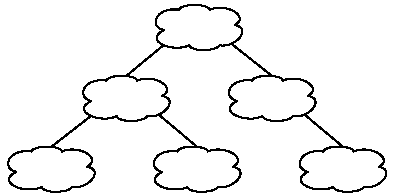
\includegraphics[width=2.2cm]{../img/tree.pdf} \\
\Emph{Graf}  & 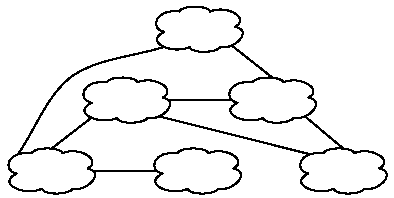
\includegraphics[width=2.2cm]{../img/graph.pdf} \\
\end{tabular}
\end{itemize}
{
\SlideFontTiny \vspace{1em }\hskip2em
Mer om listor \& träd \href{http://cs.lth.se/edaa01vt}{fördjupningskursen}. 
Mer om träd, grafer i \href{http://cs.lth.se/edaa40}{Diskreta strukturer.}
}

\end{Slide} 


\begin{Slide}{Vad är en vektor?}\SlideFontSmall
En \Emph{vektor}\footnote{Vektor kallas ibland på svenska även \href{https://sv.wikipedia.org/wiki/F\%C3\%A4lt_\%28datastruktur\%29}{fält}, men det skapar stor förvirring eftersom det engelska ordet \emph{field} ofta används för \emph{attribut} (förklaras senare).} 
\Eng{vector, \href{https://en.wikipedia.org/wiki/Array_data_structure}{array}} är en \Emph{samling} som är \Alert{snabb} att \Emph{indexera} i. 
Åtkomst av element sker med \code{apply(platsnummer)}: 

\begin{REPL}
scala> val heltal = Vector(42, 13, -1, 0 , 1)
heltal: scala.collection.immutable.Vector[Int] = Vector(42, 13, -1, 0, 1)

scala> heltal.apply(0)
res0: Int = 42

scala> heltal(1)    // man kan skippa .apply
res1: Int = 13

scala> heltal(5)
java.lang.IndexOutOfBoundsException: 5
  at scala.collection.immutable.Vector.checkRangeConvert(Vector.scala:132)
\end{REPL}
Utelämnar du \code{.apply} så gör kompilatorn anrop av \code{apply} ändå om det går.
\end{Slide}

\begin{Slide}{En konceptuell bild av en vektor}

\begin{REPLnonum}
scala> val heltal = Vector(42, 13, -1, 0 , 1)

scala> heltal(0)
res0: Int = 42
\end{REPLnonum}

\begin{tikzpicture}[font=\ttfamily]
\matrix [matrix of nodes, row sep=0, column 2/.style={nodes={rectangle,draw,minimum width=3em}}] (var) at (0cm, 2.8cm)
{
heltal   &  \makebox(16,12){ }\\
};
\matrix [matrix of nodes, draw=black,row sep=0, column 2/.style={nodes={rectangle,draw,minimum width=4em}}] (vec) at (4cm, 1cm)
{
\textit{plats} &  \\
0   &  \makebox(16,12){42}\\
1   &  \makebox(16,12){13}\\
2   &  \makebox(16,12){-1}\\
3   &  \makebox(16,12){0}\\
4   &  \makebox(16,12){1}\\
};
\filldraw[black] (0.7cm,2.8cm) circle (3pt) node[] (ref) {};
 \draw [arrow] (ref) -- (vec);
\end{tikzpicture}

%\vspace{1em} Elementen ligger på rad någonstans i minnet.
\end{Slide}



\begin{Slide}{En samling strängar}

\begin{itemize}
\item En vektor kan lagra många värden av samma typ. 
\item Elementen kan vara till exempel heltal eller strängar. 
\item Eller faktiskt vad som helst. 
\end{itemize}

\begin{REPL}
scala> val grönsaker = Vector("gurka","tomat","paprika","selleri")
grönsaker: scala.collection.immutable.Vector[String] = Vector(gurka, tomat, paprika, selleri)

scala> val g = grönsaker(1)
g: String = tomat

scala> val xs = Vector(42, "gurka", true, 42.0)
xs: scala.collection.immutable.Vector[Any] = Vector(42, gurka, true, 42.0)


\end{REPL}

\end{Slide}

\begin{Slide}{Vad är en kontrollstruktur?}
\begin{itemize}
\item En \Emph{kontrollstruktur} påverkar \Alert{sekvensen}.
\begin{itemize}
\item[] Exempel på inbyggda kontrollstrukturer: 
\\\vspace{0.5em}\code{for}-sats, \code{while}-sats
\end{itemize}

\item[]

\item I Scala kan man definiera \Emph{egna} kontrollstrukturer.
\begin{itemize}
\item[] Exempel: \code{upprepa} som du använt i Kojo
\\\vspace{0.5em}\code|upprepa(4){fram; höger}|
\end{itemize}
\end{itemize}
\end{Slide}


\begin{Slide}{Mitt första program: en oändlig loop på ABC80}
\begin{columns}
\begin{column}{0.8\textwidth}
\begin{verbatim}
10 print "hej"
20 goto 10
\end{verbatim}
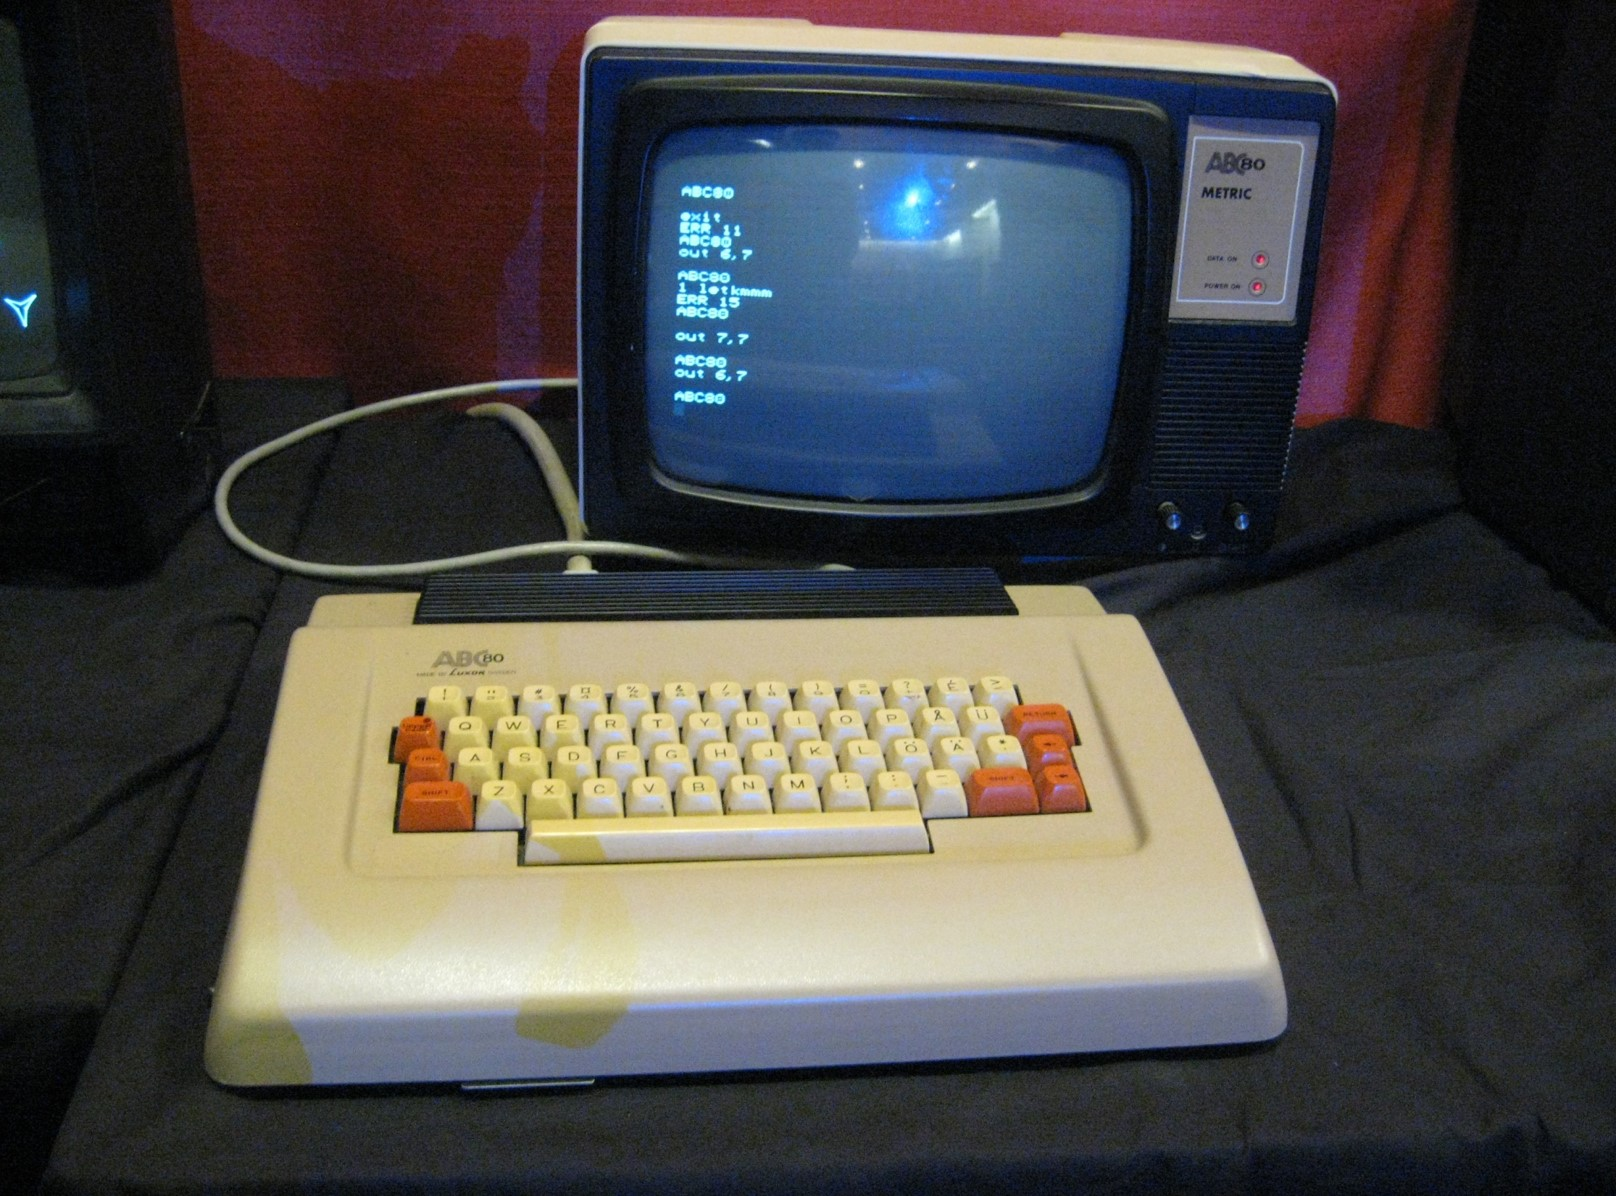
\includegraphics[width=0.8\textwidth]{../img/abc80.jpg}
\end{column}
\begin{column}{0.3\textwidth}
\pause
\begin{verbatim}
hej
hej
hej
hej
hej
hej
hej
hej
hej
hej
hej
hej
<Ctrl+C>
\end{verbatim}

\end{column}
\end{columns}
\end{Slide}


\begin{Slide}{Loopa genom elementen i en vektor}
En \code{for}-\Emph{sats} som skriver ut alla element i en vektor:
\begin{REPL}
scala> val grönsaker = Vector("gurka","tomat","paprika","selleri")

scala> for (g <- grönsaker) println(g)
gurka
tomat
paprika
selleri

\end{REPL}

\end{Slide}


\begin{Slide}{Bygga en ny samling från en befintlig med for-uttryck}
Ett \code{for}-\code{yield}-\Emph{uttryck} som \Emph{skapar en \Alert{ny} samling}.

\begin{Code}[basicstyle=\ttfamily\fontsize{12}{14}\selectfont]
for (g <- grönsaker) yield "god " + g
\end{Code}

\begin{REPL}
scala> val grönsaker = Vector("gurka","tomat","paprika","selleri")

scala> for (g <- grönsaker) yield "god " + g
res0: scala.collection.immutable.Vector[String] = 
  Vector(god gurka, god tomat, god paprika, god selleri)

scala> val åsikter = for (g <- grönsaker) yield s"god $g"
åsikter: scala.collection.immutable.Vector[String] = 
  Vector(god gurka, god tomat, god paprika, god selleri)
\end{REPL}

\end{Slide}


\begin{Slide}{Samlingen \code{Range} håller reda på intervall}
\begin{itemize}
\item Med en \code{Range(start, slut)} kan du skapa ett intervall: \\ från och med \code{start} till (men inte med) \code{slut}
\end{itemize}

\begin{REPLnonum}
scala> Range(0, 42)
res0: scala.collection.immutable.Range = 
  Range(0, 1, 2, 3, 4, 5, 6, 7, 8, 9, 10, 11, 12, 13, 14, 
    15, 16, 17, 18, 19, 20, 21, 22, 23, 24, 25, 26, 27, 28, 
    29, 30, 31, 32, 33, 34, 35, 36, 37, 38, 39, 40, 41)
\end{REPLnonum}

\begin{itemize}
\item Men alla värden däremellan skapas inte förrän de behövs:
\end{itemize}

\begin{REPL}
scala> val jättestortIntervall = Range(0, Int.MaxValue)
jättestortIntervall: scala.collection.immutable.Range = Range(0, 1, 2, 3, 4, 5, ...

scala> jättestortIntervall.end
res1: Int = 2147483647

scala> jättestortIntervall.toVector
java.lang.OutOfMemoryError: GC overhead limit exceeded
\end{REPL}

\end{Slide}

\begin{Slide}{Loopa med Range}
\code{Range} används i for-lopar för att hålla reda på antalet rundor.
\begin{REPLnonum}
scala> for (i <- Range(0, 6)) print(" gurka " + i)
 gurka 0 gurka 1 gurka 2 gurka 3 gurka 4 gurka 5 
\end{REPLnonum}
Du kan skapa en \code{Range} med \code{until} efter ett heltal:
\begin{REPLnonum}
scala> 1 until 7
res1: scala.collection.immutable.Range = 
  Range(1, 2, 3, 4, 5, 6)

scala> for (i <- 1 until 7) print(" tomat " + i) 
 tomat 1 tomat 2 tomat 3 tomat 4 tomat 5 tomat 6

\end{REPLnonum}
\end{Slide}

\begin{Slide}{Loopa med Range skapad med \texttt{to}}

Med \code{to} efter ett heltal får du en \code{Range} till och \Emph{med} sista:
\begin{REPLnonum}
scala> 1 to 6
res2: scala.collection.immutable.Range.Inclusive = 
  Range(1, 2, 3, 4, 5, 6)

scala> for (i <- 1 to 6) print(" gurka " + i) 
 gurka 1 gurka 2 gurka 3 gurka 4 gurka 5 gurka 6
 
\end{REPLnonum}


\end{Slide}



\begin{Slide}{Vad är en \code{Array} i JVM?}


\begin{itemize}
\item En \code{Array} liknar en \code{Vector} men har en särställning i JVM:
\begin{itemize}
\item Lagras som en sekvens i minnet på efterföljande adresser.
\item \Emph{Fördel}: snabbaste samlingen för element-access i JVM.
\item Men det finns en hel del \Alert{nackdelar} som vi ska se senare.
\end{itemize}

\end{itemize}

\begin{REPLnonum}
scala> val heltal = Array(42, 13, -1, 0 , 1)
\end{REPLnonum}

\begin{tikzpicture}[font=\ttfamily,scale=0.75, every node/.style={scale=0.75}]
\matrix [matrix of nodes, row sep=0, column 2/.style={nodes={rectangle,draw,minimum width=3em}}] (var) at (0cm, 2.8cm)
{
heltal   &  \makebox(16,12){ }\\
};
\matrix [matrix of nodes, draw=black,row sep=0, column 2/.style={nodes={rectangle,draw,minimum width=4em}}] (vec) at (4cm, 1cm)
{
\textit{plats} &  \\
0   &  \makebox(16,12){42}\\
1   &  \makebox(16,12){13}\\
2   &  \makebox(16,12){-1}\\
3   &  \makebox(16,12){0}\\
4   &  \makebox(16,12){1}\\
};
\filldraw[black] (0.7cm,2.8cm) circle (3pt) node[] (ref) {};
 \draw [arrow] (ref) -- (vec);
\end{tikzpicture}
\end{Slide}

\begin{Slide}{Några likheter \& skillnader mellan \texttt{Vector} och \texttt{Array}}\SlideFontSmall
\begin{multicols}{2}
\begin{REPL}[numbers=none]
scala> val xs = Vector(1,2,3)
\end{REPL}

\columnbreak

\begin{REPL}[numbers=none]
scala> val xs = Array(1,2,3)
\end{REPL}
\end{multicols}


Några likheter mellan \texttt{Vector} och \texttt{Array}
\begin{itemize}
\item Båda är samlingar som kan innehålla många element.

\item Med båda kan man snabbt accessa vilket element som helst: \code{xs(2)}

\item Båda har en fix storlek efter allokering.
\end{itemize}

Några viktiga skillnader:
\begin{multicols}{2}
\Emph{Vector}
\begin{itemize}
\item Är \Emph{oföränderlig}: du kan lita på att elementreferenserna aldrig någonsin kommer att ändras.

\item Är \Emph{snabb på att skapa en delvis förändrad kopia}, t.ex. tillägg/borttagning/uppdatering mitt i sekvensen.

\end{itemize}


\columnbreak

\Alert{Array}
\begin{itemize}
\item Är \Alert{föränderlig}: \code{xs(2) = 42}

\item Är \Alert{snabb} om man bara vill läsa eller skriva på befintliga platser.

\item Är \Alert{långsam} om man vill lägga till eller ta bort element mitt i sekvensen.

\end{itemize}
\end{multicols}
\end{Slide}



\Subsection{Huvudprogram med \texttt{main} i Scala och Java}

\begin{Slide}{Ett minimalt fristående program i Scala och Java}
Nedan Scala-kod skrivs i en editor, spara med valfritt filnamn:
\begin{Code}
// this is Scala 

object Hello {
  def main(args: Array[String]): Unit = {
    println("Hejsan scala-appen!")
  }
}
\end{Code}

\pause
\vspace{1em}
Nedan Java-kod skrivs i en editor, filen \Alert{måste} heta \texttt{Hi.java}

\begin{Code}[language=Java]
// this is Java 

public class Hi {
    public static void main(String[] args) {
        System.out.println("Hejsan Java-appen!");
    }
}
\end{Code}

\end{Slide}


\begin{Slide}{Loopa genom en samling med en \texttt{while}-sats}
\begin{REPLnonum}
scala> val xs = Vector("Hej","på","dej","!!!")
xs: scala.collection.immutable.Vector[String] = 
  Vector(Hej, på, dej, !!!)

scala> xs.size
res0: Int = 4

scala> var i = 0
i: Int = 0

scala> while (i < xs.size) { println(xs(i)); i = i + 1 }
Hej
på
dej
!!!
\end{REPLnonum}
\end{Slide}


\begin{Slide}{Loopa genom argumenten i ett Scala-huvudprogram}
Skriv denna kod och spara i filen \texttt{helloargs.scala}
\begin{REPL}[numbers=none]
$ gedit helloargs.scala
\end{REPL}
\begin{Code}
object HelloScalaArgs {
  def main(args: Array[String]): Unit = {
    var i = 0
    while (i < args.size) { 
      println(args(i))
      i = i + 1
    }
  }
}
\end{Code}
Kompilera och kör:
\begin{REPL}
$ scalac helloargs.scala
$ scala HelloScalaArgs hej gurka tomat 
hej
gurka
tomat
\end{REPL}
\end{Slide}


\begin{Slide}{Loopa genom argumenten i ett Java-huvudprogram}
\begin{REPL}[numbers=none]
$ gedit HelloJavaArgs.java
\end{REPL}
\begin{Code}[language=Java]
// this is Java 

public class HelloJavaArgs {
    public static void main(String[] args) {
    int i = 0;
    while (i < args.length) { 
      System.out.println(args[i]);
      i = i + 1;
    }
  }
}
\end{Code}
Kompilera och kör:
\begin{REPL}
$ javac HelloJavaArgs.scala
$ java HelloJavaArgs hej gurka tomat 
hej
gurka
tomat
\end{REPL}

\end{Slide}


\begin{Slide}{Scala-skript}
\begin{itemize}
\item Skala-kod kan köras som ett \Emph{skript}.\footnote{\SlideFontTiny Du får prova detta på övningen. Vi kommer mest att köra kompilerat i kursen, då Scala-skript saknar mekanism för inkludering av andra skript. Men det finns ett öppenkällkodsprojekt som löser det: \url{http://www.lihaoyi.com/Ammonite/}
}
\item Ett skript kompileras varje gång innan det körs och maskinkoden sparas inte som vid vanlig kompilering.
\item Då behövs ingen \code{main} och inget \code{object}
\end{itemize}

\begin{Code}[basicstyle=\ttfamily\fontsize{10}{12}\selectfont]
// spara nedan i filen 'myscript.scala'

println("Hejsan argumnet!")
for (arg <- args) println(arg)
\end{Code}

\begin{REPLnonum}
$ scala myscript.scala
\end{REPLnonum}


\end{Slide}



\Subsection{Algoritmer: stegvisa lösningar}

\begin{Slide}{Vad är en algoritm?}
En \href{https://sv.wikipedia.org/wiki/Algoritm}{algoritm} är en sekvens av instruktioner som beskriver \\hur man löser ett problem.\\
\vspace{1em}
\Emph{Exempel}: 
\begin{itemize}
\item	 baka en kaka 
\pause\item räkna ut din pensionsprognos 
\pause\item köra bil 
\pause\item kolla om highscore i ett spel 
\item ...
\end{itemize}

\begin{tikzpicture}[overlay]
\node[xshift=0.85\textwidth, scale=2.0] at (0,1.3) { 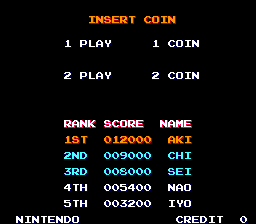
\includegraphics[width=0.25\textwidth]{../img/highscore}};
\end{tikzpicture}
\end{Slide}



\begin{Slide}{Algoritm-exempel: HIGHSCORE}
\Emph{Problem}: Kolla om high-score i ett spel \\ \vspace{1em}

\Emph{Varför?} \pause Så att de som spelar uppmuntras att spela mer :) \\ \vspace{1em}

\Emph{Algoritm:}\pause
\begin{enumerate}
\item $points$ $\leftarrow$ poängen efter senaste spelet
\item $highscore$ $\leftarrow$ bästa resultatet innan senaste spelet
\item \Key{om} $points$ är större än $highscore$ 
\begin{enumerate}[ ~~]
\item  Skriv ''Försök igen!''
\end{enumerate}
\Key{annars}
\begin{enumerate}[ ~~]
\item  Skriv ''Grattis!''
\end{enumerate}
\end{enumerate}
\pause
\scriptsize \Alert{Hittar du buggen?}
\end{Slide}


\begin{Slide}{HIGHSCORE implementerad i Scala}
\begin{Code}
import scala.io.StdIn.readLine

object HighScore {
  def main(args: Array[String]): Unit = {
    val points = readLine("Hur mång poäng fick du?").toInt
    val highscore = readLine("Vad var highscore före senaste spelet?").toInt
    val msg = if (points > highscore) "GRATTIS!" else "Försök igen!"
    println(msg) 
  }
}
\end{Code}
\pause
Är det en bugg eller en feature att det står\\ \texttt{points > highscore} \\ och inte \\ \texttt{points >= highscore} \\ ?
% Buggen är att man inte får GRATTIS om poäng == highscore vilket är tråkigt :)
\end{Slide}


\begin{Slide}{HIGHSCORE implementerad i Java}
\begin{Code}[language=Java]
import java.util.Scanner;

public class HighScore {
    public static void main(String[] args){
        Scanner scan = new Scanner(System.in);
        System.out.println("Hur många poäng fick du?");
        int points =  scan.nextInt();
        System.out.println("Vad var higscore före senaste spelet?");
        int highscore = scan.nextInt();
        if (points > highscore) {
            System.out.println("GRATTIS!");
        } else {
            System.out.println("Försök igen!");
        }
    }
}
\end{Code}
\end{Slide}


\begin{Slide}{Algoritmexempel: N-FAKULTET}
\begin{algorithm}[H]
 \SetKwInOut{Input}{Indata}\SetKwInOut{Output}{Resultat}

 \Input{heltalet $n$}
 \Output{utskrift av produkten av de första $n$ heltalen }
 ~\\
 $prod \leftarrow 1$ \\
 $i \leftarrow 2$  \\
 \While{$i \leq n$}{
  $prod \leftarrow prod * i$\\
  $i \leftarrow i + 1$
 }
 skriv ut $prod$
\end{algorithm}
\pause\vspace{1em}
\begin{itemize}\SlideFontSmall
\item Vad händer om $n$ är noll?
\item Vad händer om $n$ är ett?
\item Vad händer om $n$ är två?
\item Vad händer om $n$ är tre?
\end{itemize}
\end{Slide}

\begin{Slide}{Algoritmexempel: MIN}
\begin{algorithm}[H]
 \SetKwInOut{Input}{Indata}\SetKwInOut{Output}{Resultat}

 \Input{Array $args$ med strängar som alla innehåller heltal}
 \Output{utskrift av minsta heltalet }
 ~\\
 $min \leftarrow$ det största heltalet som kan uppkomma  \\
 $n \leftarrow $ antalet heltal \\
 $i \leftarrow 0$ \\
 \While{$i < n$}{
   $x \leftarrow args(i).toInt$ \\
   \If{( x < $min$)}{$min \leftarrow x$}
   $i \leftarrow i + 1$
 }
 skriv ut $min$
\end{algorithm}
\pause{\hfill \SlideFontTiny \Emph{Test med indata}: \code{args = Array("2", "42", "1", "2")}}
\end{Slide}


\Subsection{Funktioner skapar struktur}

\begin{Slide}{Mall för funktionsdefinitioner}

\code{def} funktionsnamn(parameterdeklarationer): returtyp = block

\pause\vspace{0.5em}\Emph{Exempel}:

\begin{Code}[basicstyle=\ttfamily\fontsize{9}{11}\selectfont]
def öka(i: Int): Int = { i + 1 }
\end{Code}
\pause Om ett enda uttryck: behövs inga \code|{}|. Returtypen kan härledas.
\begin{Code}[basicstyle=\ttfamily\fontsize{9}{11}\selectfont]
def öka(i: Int) = i + 1  
\end{Code}
\pause Om flera parametrar, separera dem med kommatecken: 
\begin{Code}[basicstyle=\ttfamily\fontsize{9}{11}\selectfont]
def isHighscore(points: Int, high: Int): Boolean = {
  val highscore: Boolean = points > high
  if (highscore) println(":)") else print(":(")
  highscore
}
\end{Code}
\pause Ovan funktion har \Alert{sidoeffekten} att skriva ut en smiley.
\end{Slide}

\begin{Slide}{Bättre många små abstraktioner som gör en sak var}

\begin{Code}[basicstyle=\ttfamily\fontsize{8}{11}\selectfont]
def isHighscore(points: Int, high: Int): Boolean = points > high

def printSmiley(isHappy: Boolean): Unit = 
  if (isHappy) println(":)") else print(":(")
\end{Code}

\pause\vspace{2em}
\begin{REPLnonum}
  printSmiley(isHighscore(113,99))
\end{REPLnonum}

\pause\vspace{2em} \code{isHigscore} är en \Emph{äkta funktion} som alltid ger samma svar för samma inparametrar och saknar \Alert{sidoeffekter}.

\end{Slide}



\begin{Slide}{Vad är ett block?}

\begin{itemize}
\item Ett block \Emph{kapslar in} flera satser/uttryck och ser ''utifrån'' ut som en enda sats/uttryck.

\item Ett block skapas med hjälp av klammerparenteser (''krullparenteser'')

\item [] {\fontsize{14}{18}\selectfont \code|{ uttryck1; uttryck2; ... uttryckN }|}\\~

\pause

\item I Scala (till skillnad från många andra språk) har ett block ett \Emph{värde} och är alltså ett \Emph{uttryck}. 

\item Värdet ges av \Emph{sista uttrycket}.

\begin{REPLnonum}
scala> val x = { println(1 + 1); println(2 + 2); 3 + 3 } 
2
4
x: Int = 6
\end{REPLnonum}


\end{itemize}

\end{Slide}

\begin{Slide}{Namn i block blir \textbf{lokala}}
Synlighetsregler: 
\begin{enumerate}
\item Identifierare deklarerade inuti ett block blir \Emph{lokala}.

\item Lokala namn \Alert{överskuggar} namn i yttre block om samma.


\item Namn syns i nästlade underblock.

\end{enumerate}

\begin{REPL}
scala> { val lokaltNamn = 42; println(lokaltNamn) }
42

scala> println(lokaltNamn)
<console>:12: error: not found: value lokaltNamn
       println(lokaltNamn)

scala> { val x = 42; { val x = 76; println(x) }; println(x) }
76
42

scala> { val x = 42; { val y = x + 1; println(y) } }
43
\end{REPL}

\end{Slide}


\begin{Slide}{Parameter och argument}

Skilj på parameter och argument!
\begin{itemize}
\item En \Alert{parameter} är det deklarerade namnet som används \Alert{lokalt} i en funktion för att referera till...

\item \Emph{argumentet} som är värdet som skickas med \Emph{vid anrop} och binds till det lokala parameternamnet.

\end{itemize}


\begin{REPLnonum}
scala> val ettArgument = 42

scala> def öka(minParameter: Int) = minParameter + 1

scala> öka(ettArgument)
\end{REPLnonum}


Speciell syntax: anrop med s.k. \Emph{namngiven parameter}
\begin{REPLnonum}
scala> öka(minParameter = ettArgument) 
\end{REPLnonum}

\end{Slide}

\begin{Slide}{Procedurer}\SlideFontSmall
\begin{itemize}
\item En \Emph{procedur} är en funktion som \Alert{gör} något intressant, men som \Alert{inte} lämnar något intressant returvärde.
\item Exempel på befintlig procedur: \code{println("hej")}
\item Du \Emph{deklarerar egna procedurer} genom att ange \texttt{\Alert{Unit}} som returvärdestyp. Då ges värdet \texttt{\Alert{()}} som betyder ''inget''.
\end{itemize}
\begin{REPL}
scala> def hej(x: String): Unit = println(s"Hej på dej $x!")
hej: (x: String)Unit

scala> hej("Herr Gurka")
Hej på dej Herr Gurka!

scala> val x = hej("Fru Tomat")
Hej på dej Fru Tomat!
x: Unit = ()
\end{REPL}
\begin{itemize}
\item Det som \Alert{görs} kallas (sido)\Emph{effekt}. Ovan är utskriften själva effekten.
\item Funktioner kan också ha sidoeffekter. De kallas då \Alert{oäkta} funktioner.
\end{itemize}
\end{Slide}

\begin{Slide}{''Ingenting'' \emph{är} faktiskt någonting i Scala}
\begin{itemize}
\item I många språk (Java, C, C++, ...) är funktioner som saknar värden speciella.
 Java m.fl. har speciell syntax för procedurer med nyckelordet \jcode{void}, men \Alert{inte} Scala. 

\item I Scala är procedurer inte specialfall; de är vanliga funktioner som returnerar ett värde som \Emph{representerar} ingenting, nämligen () som är av typen Unit. 

\item På så sätt blir procedurer inget undantag utan följer vanlig syntax och semantik precis som för alla andra funktioner.

\item Detta är typiskt för Scala: generalisera koncepten och vi slipper besvärliga undantag! \\(Men vi måste förstå generaliseringen...)


\item [] {\SlideFontSmall 
\url{https://en.wikipedia.org/wiki/Void_type}
\url{https://en.wikipedia.org/wiki/Unit_type}
}

\end{itemize}

\end{Slide}

\begin{Slide}{Abstraktion: Problemlösning genom nedbrytning i enkla funktioner och procedurer som kombineras}\SlideFontSmall
\begin{itemize}
\item En av de allra viktigaste principerna inom programmering är \Emph{funktionell nedbrytning} där  \Emph{underprogram} i form av funktioner och procedurer skapas för att bli byggstenar som kombineras till mer avancerade funktioner och procedurer.

\item Genom de namn som definieras skapas \Emph{återanvändbara abstraktioner} som kapslar in det funktionen gör. 

\item Problemet blir med bra byggblock lättare att lösa.

\item Abstraktioner som beräknar eller gör \Emph{en enda, väldefinierad sak} är enklare att använda, jämfört med de som gör många, helt olika saker.

\item Abstraktioner med \Emph{välgenomtänkta namn} är enklare att använda, jämfört med kryptiska eller missvisande namn.
\end{itemize}

\end{Slide}



\begin{Slide}{Exempel på \textbf{funktionell nedbrytning}}

Kojo-labben gav exempel på \Emph{funktionell nedbrytning} där ett antal abstraktioner skapas och återanvänds.

\begin{Code}
// skapa abstraktioner som bygger på varandra

def kvadrat = upprepa(4){fram; höger}

def stapel = {
  upprepa(10){kvadrat; hoppa}
  hoppa(-10*25)
}

def rutnät = upprepa(10){stapel; höger; fram; vänster}

// huvudprogram 

sudda; sakta(200)
rutnät
\end{Code}
\end{Slide}


\begin{Slide}{Varför abstraktion?}
\begin{itemize}
\item Stora program behöver delas upp annars blir det mycket svårt att förstå och bygga vidare på programmet.
\item Vi behöver kunna välja namn på saker i koden \textit{lokalt}, utan att det krockar med samma namn i andra delar av koden.
\item Abstraktioner hjälper till att hantera och kapsla in komplexa delar så att de blir enklare att använda om och om igen. 

\item Exempel på \Emph{abstraktionsmekanismer} i Scala och Java:
\begin{itemize}

\item \href{https://sv.wikipedia.org/wiki/Klass_\%28programmering\%29}{Klasser} är ''byggblock'' med kod som används för att skapa \href{https://sv.wikipedia.org/wiki/Objektorienterad_programmering\#Objekt}{objekt}, innehållande delar som hör ihop. \\ Nyckelord: \code{class} och \code{object} 

\item \href{https://en.wikipedia.org/wiki/Method_\%28computer_programming\%29}{Metoder} är funktioner som finns i klasser/objekt och används för att lösa specifika uppgifter.  Nyckelord: \code{def}

\item \href{https://en.wikipedia.org/wiki/Java_package}{Paket} används för att organisera kodfiler i en hierarkisk katalogstruktur och skapa namnrymder. \\Nyckelord: \Key{package}

\end{itemize}

\end{itemize}
\end{Slide}


\Subsection{Katalogstruktur för kodfiler med paket}



\begin{Slide}{Källkodsfiler och klassfiler}
\begin{tikzpicture}[node distance=1.5cm]
\node (input) [startstop] {\texttt{Hello.scala}};
\node(inptext) [right of=input, text width=5cm, scale=1.2,xshift=3.5cm]{Källkodsfil};
\node (compile) [process, below of=input] {\texttt{scalac}};
\node (output) [startstop, below of=compile] {\texttt{Hello.class}};
\node(outtext) [right of=output, text width=5cm, scale=1.2,xshift=3.5cm]{\texttt{.class}-fil med byte-kod};
\node (jvm) [process, below of=output] {JVM};
\node(jvmtext) [right of=jvm, text width=5.5cm, scale=0.8,xshift=4.5cm]{\textit{Java Virtual Machine}\\Översätter till maskinkod\\ som passar din specifika CPU\\medan programmet kör};
\draw [arrow] (input) -- (compile);
\draw [arrow] (compile) -- (output);
\draw [arrow] (output) -- (jvm);
\end{tikzpicture}
\end{Slide}




\begin{Slide}{Paket}\SlideFontSmall
\begin{itemize}
\item Paket ger struktur åt kodfilerna. Bra om man har många kodfiler.

\item Byte-koden placeras av kompilatorn i kataloger enligt paketstrukturen.


\end{itemize}

\vspace{1em}
\begin{tikzpicture}[node distance=1.5cm,scale=0.8, every node/.style={transform shape}]
\node (input) [startstop] {\texttt{greeting/Hello.scala}};
\node(inptext) [right of=input, text width=4cm, scale=1.2,xshift=4.5cm]{\lstinline{package greeting}\\\lstinline{object Hello { ... }};
\node (compile) [process, below of=input] {\texttt{scalac  greeting/Hello.java}};
\node (output) [startstop, below of=compile] {\texttt{greeting/Hello.class}};
\node(outtext) [right of=output, text width=4cm, scale=1.2,xshift=4.5cm]{Paketens bytekod hamnar i katalog med samma namn som paketnamnet};
\node (jvm) [process, below of=output] {\texttt{scala greeting.Hello}};
\draw [arrow] (input) -- (compile);
\draw [arrow] (compile) -- (output);
\draw [arrow] (output) -- (jvm);
\end{tikzpicture}

{\SlideFontTiny\vspace{1em} Katalogstrukturen för källkoden måste i Java motsvara paketstrukturen, \\men inte i Scala. Dock kräver många IDE att så görs även för Scala.}
\end{Slide}

\begin{Slide}{Import}
Med hjälp av punktnotation kommer man åt innehåll i ett paket.\\
\begin{Code}
val age = scala.io.StdIn.readLine("Ange din ålder:")
\end{Code}

En \code{import}-sats...
 
\begin{Code}
import scala.io.StdIn.readLine
\end{Code}

...gör så att kompilatorn ''ser'' namnet, och man slipper skriva hela sökvägen till namnet:
\begin{Code}
val age = readLine("Ange din ålder:")
\end{Code}

Man säger att det importerade namnet hamnar \Emph{\textit{in scope}}.
\end{Slide}





\begin{Slide}{Jar-filer}
\texttt{jar}-filer liknar \texttt{zip}-filer och används för att packa ihop bytekod i en enda fil för enkel distribution och körning. 

\vspace{2em}
\begin{tikzpicture}[node distance=1.5cm,scale=0.8, every node/.style={transform shape}]
\node (input) [startstop] {\texttt{greeting/}};
\node(inptext) [right of=input, text width=4cm, scale=1.2,xshift=4.5cm]{en katalog med filer};
\node (jar) [process, below of=input] 
{\texttt{jar cvf minjarfil.jar greeting}};

\node (output) [startstop, below of=compile] {\texttt{minjarfil.jar}};

\node(outtext) [right of=output, text width=4cm, scale=1.2,xshift=4.5cm]{En jar-fil med alla filer inpackade};

\node (jvm) [process, below of=output] {\texttt{scala -cp minjarfil.jar}};

\node(outtextjvm) [right of=jvm, text width=4cm, scale=1.2,xshift=4.5cm]{Lägg jar-filen till \\ ''classpath''};
\draw [arrow] (input) -- (jar);
\draw [arrow] (jar) -- (output);
\draw [arrow] (output) -- (jvm);
\end{tikzpicture}
\end{Slide}

\Subsection{Dokumentation}

\begin{Slide}{Dokumentation}\footnotesize
För att kod ska bli begriplig för människor är det bra att dokumentera vad den gör. Det finns \Emph{tre olika sorters kommentarer} som man kan skriva direkt i Scala/Java-koden, \Alert{som kompilatorn struntar fullständigt i}:
\begin{lstlisting}
// Enradskommentarer börjar med dubbla snedstreck
//       men de gäller bara till radslut

/* Flerradskommentarer börjar med 
   snedstreck-asterisk
   och slutar med asterisk-snedstreck.  */ 

/** Dokumentationskommentarer placeras före 
 *   t.ex. en funktion och berättar vad den gör
 *   och vad eventuella parametrar används till.
 *   Börjar med snedstreck-asterisk-asterisk.
 *   Varje ny kommentarsrad börjar med asterisk.
 *   Avslutas med asterisk-stjärna.
 */
\end{lstlisting}
\end{Slide}

\begin{Slide}{scaladoc}
Programmet \texttt{scaladoc}-filer läser källkod och skapar en webbsajt med dokumentation. 

\vspace{2em}
\begin{tikzpicture}[node distance=1.5cm,scale=0.8, every node/.style={transform shape}]

\node (input) [startstop] {\texttt{greeting/}};

\node(inptext) [right of=input, text width=4cm, scale=1.2,xshift=4.5cm]{en katalog med \texttt{.scala}-filer};

\node (scaladoc) [process, below of=input] 
{\texttt{scaladoc greeting/*.scala}};

\node (output) [startstop, below of=compile] {\texttt{index.html} ~~med mera...};

\node(outtext) [right of=output, text width=4cm, scale=1.2,xshift=4.5cm]{En webbsajt};


\draw [arrow] (input) -- (scaladoc);
\draw [arrow] (scaladoc) -- (output);
\end{tikzpicture}
\end{Slide}



\subsection{Att göra denna vecka}


%%%
\begin{Slide}{Att göra i Vecka \vecka: Förstå grundläggande kodstrukturer}

\begin{enumerate}
\item Laborationer är \Alert{obligatoriska}.\\ Ev. sjukdom måste anmälas \Alert{före} via mejl till kursansvarig!
\item Gör övning \texttt{programs}
\item OBS! Ingen lab denna vecka w02. Använd tiden att komma ikapp om du ligger efter!
\item Träffas i samarbetsgrupper och hjälp varandra att förstå.
\item Vi har nosat på flera koncept som vi kommer tillbaka till senare: du måste inte fatta alla detaljer redan nu.
\item Om ni inte redan gjort det: \\Visa \href{https://github.com/bjornregnell/lth-eda016-2015/tree/master/assignments}{samarbetskontrakt} för handledare på resurstid.
\item \Alert{Koda på resurstiderna} och få hjälp och tips! 
\end{enumerate}
\end{Slide}

\begin{Slide}{Veckans övning: \code{w02-programs}}\SlideFontTiny
\vspace{-0.5em}
\setlength{\leftmargini}{0pt}
\begin{itemize}
%!TEX encoding = UTF-8 Unicode
%!TEX root = ../compendium2.tex

\item Kunna skapa samlingarna Range, Array och Vector med heltals- och strängvärden.
\item Kunna indexera i en indexerbar samling, t.ex. Array och Vector.
\item Kunna anropa operationerna size, mkString, sum, min, max på samlingar som innehåller heltal.
\item Känna till grundläggande skillnader och likheter mellan samlingarna Range, Array och Vector.
\item Förstå skillnaden mellan en for-sats och ett for-uttryck.
\item Kunna skapa samlingar med heltalsvärden som resultat av enkla for-uttryck.
\item Förstå skillnaden mellan en algoritm i pseudo-kod och dess implementation.
\item Kunna implementera algoritmerna SUM, MIN/MAX på en indexerbar samling med en \code{while}-sats.
\item Kunna köra igång enkel Scala-kod i REPL, som skript och som applikation.
\item Kunna skriva och köra igång ett enkelt Java-program.
\item Känna till några grundläggande syntaxskillnader mellan Scala och Java, speciellt variabeldeklarationer och indexering i Array.
\item Förstå vad ett block och en lokal variabel är.
\item Förstå hur nästlade block påverkar namnsynlighet och namnöverskuggning.
\item Förstå kopplingen mellan paketstruktur och kodfilstruktur.
\item Kunna skapa en jar-fil.
\item Kunna skapa dokumentation med scaladoc.

\end{itemize}
\end{Slide}













\Lecture{3}{Funktioner, Objekt}
%!TEX encoding = UTF-8 Unicode
%!TEX root = ../lect-week03.tex


\Subsection{Funktioner}



\begin{Slide}{Deklarera funktioner, överlagring}
\begin{itemize}
\item En parameter, och sedan två parametrar:
\begin{REPL}
scala> :paste
  def öka(a: Int): Int = a + 1
  def öka(a: Int, b: Int) = a + b
  
scala> öka(1)
res0: Int = 2

scala> öka(1,1)
res1: Int = 2

\end{REPL}
\item Båda funktionerna ovan kan finnas samtidigt! Trots att de har samma namn är de \Alert{olika} funktioner; kompilatorn kan skilja dem åt med hjälp av de olika parameterlistorna.

\item Detta kallas \Emph{överlagring} \Eng{overloading} av funktioner.

\end{itemize}
\end{Slide} 


\begin{Slide}{Tom parameterlista och inga parametrar}\SlideFontSmall
\begin{itemize}
\item Om en funktion deklareras med tom parameterlista \code{()} kan den anropas på två sätt: med och utan tomma parenteser.
\begin{REPL}
scala> def tomParameterLista() = 42

scala> tomParameterLista()
res2: Int = 42

scala> tomParameterLista
res3: Int = 42
\end{REPL}

Denna flexibilitet är grunden för \Emph{enhetlig access}: namnet kan användas enhetligt oavsett om det är en funktion eller en variabel.
\item Om parameterlista saknas får man \Alert{inte} använda \code{()} vid anrop:

\begin{REPL}
scala> def ingenParameterLista = 42

scala> ingenParameterLista
res4: Int = 42

scala> ingenParameterLista()
<console>:13: error: Int does not take parameters
       ingenParameterLista()
\end{REPL}

\end{itemize}
\end{Slide} 


\begin{Slide}{Funktioner med defaultargument}\SlideFontSmall

\begin{itemize}
\item Vi kan ofta åstadkomma något som liknar överlagring, men med en enda funktion, om vi i stället använder \Emph{defaultargument}:
\begin{REPLnonum}
scala> def inc(a: Int, b: Int = 1) = a + b
inc: (a: Int, b: Int)Int

scala> inc(42, 2)
res0: Int = 44

scala> inc(42, 1)
res1: Int = 43

scala> inc(42)
res2: Int = 43

\end{REPLnonum}
\item Om argumentet utelämnas och det finns ett defaultargumentet, så är det defaultargumentet som appliceras.
\end{itemize}
\end{Slide} 


\begin{Slide}{Funktioner med namngivna argument}
\begin{itemize}
\item Genom att använda \Emph{namngivna argument} behöver man inte hålla reda på ordningen på parametrarna, bara man känner till parameternamnen. 
\item Namngivna argument går fint att \Alert{kombinera} med defaultargument.
\begin{REPL}
scala> def namn(förnamn: String, 
                efternamn: String, 
                förnamnFörst: Boolean = true,
                ledtext: String = ""): String = 
         if (förnamnFörst) s"$ledtext: $förnamn $efternamn" 
         else s"$ledtext: $efternamn, $förnamn"

scala> namn(ledtext = "Name", efternamn = "Coder", förnamn = "Kim")
res0: String = Name: Kim Coder
\end{REPL}
\end{itemize}
\end{Slide} 


\begin{Slide}{Anropsstacken och objektheapen}\SlideFontSmall
Minnet är uppdelat i två delar:
\begin{itemize}
\item \Emph{Anropsstacken}: På stackminnet läggs en \Emph{aktiveringspost} \Eng{stack frame\footnote{\href{https://en.wikipedia.org/wiki/Call_stack}{en.wikipedia.org/wiki/Call\_stack}}, activation record} för varje funktionsanrop med plats för parametrar och lokala variabler. Aktiveringsposten raderas när returvärdet har levererats. Stacken växer vid nästlade funktionsanrop, då en funktion i sin tur anropar en annan funktion. 

\item \Emph{Objektheapen}: I heapminnet\footnote{\href{https://en.wikipedia.org/wiki/Memory_management}{en.wikipedia.org/wiki/Memory\_management}}$^{,}$\footnote{Ej att förväxlas med datastrukturen heap  \href{https://sv.wikipedia.org/wiki/Heap}{sv.wikipedia.org/wiki/Heap}} sparas alla objekt (data) som allokeras under körning. Heapen städas vid tillfälle av skräpsamlaren \Eng{garbage collector}, och minne som inte används längre frigörs. \\\vspace{0.5em}
\href{http://stackoverflow.com/questions/1565388/increase-heap-size-in-java}{stackoverflow.com/questions/1565388/increase-heap-size-in-java}
\end{itemize}
\end{Slide} 


\begin{Slide}{Aktiveringspost}\SlideFontSmall
Nästlade anrop ger växande anropsstack.
\begin{REPL}
scala> :paste
def f(): Unit = { val n = 5; g(n, 2 * n) }
def g(a: Int, b: Int): Unit = { val x = 1; h(x + 1, a + b) }
def h(x: Int, y: Int): Unit = { val z = x + y; println(z) }

scala> f()

\end{REPL}

\pause
\Alert{Stacken}

\begin{tabular}{|r | l | l |} \hline

variabel & värde & Vilken aktiveringspost? \\ \hline \hline
\pause
 n & 5 & f \\ \hline
 \pause 
 a & 5 & g \\
 b & 10 &  \\
 x & 1  &  \\  \hline
 \pause 
 x & 2  & h \\
 y & 15 &  \\
 z & 17 & \\ \hline
\end{tabular}
\end{Slide} 


\begin{Slide}{Lokala funktioner}\SlideFontSmall
Med lokala funktioner kan delproblem lösas med nästlade abstraktioner. 

\begin{Code}
def gissaTalet(max: Int): Unit = {
  def gissat = io.StdIn.readLine(s"Gissa talet mellan [1, $max]: ").toInt 
  val hemlis = (math.random * max + 1).toInt
  def skrivLedtrådOmEjRätt(gissning: Int): Unit = 
    if (gissning > hemlis) println(s"$gissning är för stort :(") 
    else if (gissning < hemlis) println(s"$gissning är för litet :(")
  def inteRätt(gissning: Int): Boolean = { 
    skrivLedtrådOmEjRätt(gissning)
    gissning != hemlis
  }
  def loop: Int = { var i = 1; while(inteRätt(gissat)){ i += 1 }; i }
  
  println(s"Du hittade talet $hemlis på $loop gissningar :)")
}
\end{Code}

Lokala, nästlade funktionsdeklarationer är tyvärr inte tillåtna i Java.\footnote{\href{http://stackoverflow.com/questions/5388584/does-java-support-inner-local-sub-methods}{\SlideFontSize{8}{9}stackoverflow.com/questions/5388584/does-java-support-inner-local-sub-methods}} 

\end{Slide} 



\begin{Slide}{Värdeanrop och namnanrop}\SlideFontSmall
\begin{itemize}
\item Det vi sett hittills är \Emph{värdeanrop}: argumentet evalueras \Alert{först} innan dess \Alert{värde} \emph{sedan} appliceras:
\begin{REPL}
scala> def byValue(n: Int): Unit = for (i <- 1 to n) print(" " + n)

scala> byValue(21 + 21)
 42 42 42 42 42 42 42 42 42 42 42 42 42 42 42 42 42 42 42 42 42 42 42 42 42 42 42 42 42 42 42 42 42 42 42 42 42 42 42 42 42 42

scala> byValue({print(" hej"); 21 + 21})
 hej 42 42 42 42 42 42 42 42 42 42 42 42 42 42 42 42 42 42 42 42 42 42 42 42 42 42 42 42 42 42 42 42 42 42 42 42 42 42 42 42 42 42
\end{REPL}
\item Men man kan med \code{=>} före parametertypen åstadkomma \Emph{namnanrop}: argumentet \Alert{''klistras in''} i stället för \Alert{namnet} och evalueras \Alert{varje gång} (kallas även \Emph{fördröjd evaluering}):
\begin{REPL}
scala> def byName(n: => Int): Unit = for (i <- 1 to n) print(" " + n)

scala> byName({print(" hej"); 21 + 21})
 hej hej 42 hej 42 hej 42 hej 42 hej 42 hej 42 hej 42 hej 42 hej 42 hej 42 hej 42 hej 42 hej 42 hej 42 hej 42 hej 42 hej 42 hej 42 hej 42 hej 42 hej 42 hej 42 hej 42 hej 42 hej 42 hej 42 hej 42 hej 42 hej 42 hej 42 hej 42 hej 42 hej 42 hej 42 hej 42 hej 42 hej 42 hej 42 hej 42 hej 42 hej 42 hej 42
\end{REPL}

\end{itemize}
\end{Slide} 

\begin{Slide}{Klammerparenteser vid ensam parameter}
Så här har vi sett nyss att man man göra:
\begin{REPL}
scala> def loop(n: => Int): Unit = for (i <- 1 to n) print(" " + n)

scala> loop(21 + 21)

scala> loop({print(" hej"); 21 + 21})
\end{REPL}

Men...\\För alla funktioner \code{f} gäller att: \\ det är helt ok att byta ut vanliga parenteser: \hfill\code{f(uttryck)} \\ mot krullparenteser: \hfill\code|f{uttryck}| \\ \Alert{om} parameterlistan har \Alert{exakt en} parameter.  

\vspace{0.5em}Men man kan alltså göra så här också:
\begin{REPLnonum}
scala> loop{ 21 + 21 }

scala> loop{ print(" hej"); 21 + 21 }
\end{REPLnonum}


\end{Slide} 

\begin{Slide}{Uppdelad parameterlista}
\begin{itemize}
\item Vi har tidigare sett att man kan ha mer än en parameter:
\begin{REPLnonum}
scala> def add(a: Int, b: Int) = a + b

scala> add(21, 21)
res0: Int = 42
\end{REPLnonum}

\item Man kan även ha \Alert{mer än en} parameterlista:
\begin{REPLnonum}

scala> def add(a: Int)(b: Int) = a + b

scala> add(21)(21)
res1: Int = 42
\end{REPLnonum}
\item Detta kallas även \Emph{multipla parameterlistor} \Eng{multiple parameter lists}
\end{itemize}
\href{http://docs.scala-lang.org/style/declarations.html#multiple-parameter-lists}{\SlideFontTiny docs.scala-lang.org/style/declarations.html\#multiple-parameter-lists}
\end{Slide} 


\begin{Slide}{Skapa din egen kontrollstruktur}
\begin{itemize}
\item Genom att \Alert{kombinera} \Emph{uppdelad parameterlista} med \Emph{namnanrop} med \Emph{klammerparentes vid ensam parameter} kan vi skapa vår egen kontrollstruktur:
\begin{REPLnonum}
scala> def upprepa(n: Int)(block: => Unit) = { 
         var i = 0
         while (i < n) { block; i += 1 }
       }

scala> upprepa(42){ 
         if (math.random < 0.5) {
           print(" gurka")
         } else {
           print(" tomat")
         }
       }
 gurka gurka gurka tomat tomat gurka gurka gurka gurka tomat tomat tomat tomat tomat gurka tomat tomat tomat tomat tomat tomat tomat tomat tomat gurka gurka gurka tomat tomat gurka gurka gurka tomat tomat gurka tomat gurka gurka gurka gurka tomat tomat
\end{REPLnonum}
\end{itemize}
\end{Slide} 


\begin{Slide}{Funktioner är äkta värden i Scala}\SlideFontSmall
\begin{itemize}
\item En funktioner är ett äkta värde.
\item Vi kan till exempel tilldela en variabel ett funktionsvärde. 
\item Med hjälp av blank+understreck efter funktionsnamnet får vi funktionen som ett \Alert{värde} (inga argument appliceras än):
\begin{REPLnonum}
scala> def add(a: Int, b: Int) = a + b

scala> val f = add _

scala> f
f: (Int, Int) => Int = <function2>

scala> f(21, 21)
res0: Int = 42
\end{REPLnonum}

\item Ett funktionsvärde har en \Alert{typ} precis som alla värden: \\ 
\code{f: (Int, Int) => Int}
\end{itemize}
\end{Slide} 

\begin{Slide}{Funktionsvärden kan vara argument}
\begin{itemize}
\item En funktion kan ha en annan funktion som parameter:
\begin{REPL}
scala> def tvåGånger(x: Int, f: Int => Int) = f(f(x))

scala> def öka(x: Int) = x + 1

scala> def minska(x: Int) = x - 1

scala> tvåGånger(42, öka _)
res1: Int = 43

scala> tvåGånger(42, minska _)
res1: Int = 41
\end{REPL}

\item Om argumentets funktionstyp \Alert{kan härledas} av kompilatorn och \Alert{passar} med parametertypen så behövs ej understreck: \\ 
\begin{REPL}
scala> tvåGånger(42, öka)
res1: Int = 43
\end{REPL}\end{itemize}
\end{Slide}



\begin{Slide}{Applicera funktioner på element i samlingar med \texttt{map}}\SlideFontSmall
\begin{REPL}
scala> def öka(x: Int) = x + 1

scala> def minska(x: Int) = x - 1

scala> val xs = Vector(1, 2, 3)

scala> xs.map(öka)
res0: scala.collection.immutable.Vector[Int] = Vector(2, 3, 4)

scala> xs.map(minska)
res1: scala.collection.immutable.Vector[Int] = Vector(0, 1, 2)

scala> xs map öka
res2: scala.collection.immutable.Vector[Int] = Vector(2, 3, 4)

scala> xs map minska
res3: scala.collection.immutable.Vector[Int] = Vector(0, 1, 2)
\end{REPL}
Funktioner som tar andra funktioner som parametrar kallas \\ \Emph{högre ordningens funktioner}. 
\end{Slide} 




\begin{Slide}{Anonyma funktioner}
\begin{itemize}
\item  Man behöver inte ge funktioner namn. De kan i stället skapas med hjälp av \Emph{funktionsliteraler}.\footnote{Även kallat ''lambda-värde'' eller bara ''lamda'' efter den s.k. lambdakalkylen. \href{https://en.wikipedia.org/wiki/Anonymous_function}{en.wikipedia.org/wiki/Anonymous\_function}}

\item En funktionsliteral har ...
\begin{enumerate}
\item en parameterlista (utan funktionsnamn) och ev. returtyp, \item sedan den reserverade teckenkombinationen \code{=>} \item och sedan ett uttryck (eller ett block).
\end{enumerate}
\item Exempel:
\begin{Code}[basicstyle=\ttfamily\fontsize{10}{12}\selectfont]
(x: Int, y: Int): Int => x + y
\end{Code}
\pause
\item Om kompilatorn kan gissa typerna från sammanhanget så behöver typerna inte anges i själva  funktionsliteralen:
\begin{Code}[basicstyle=\ttfamily\fontsize{10}{12}\selectfont]
val f: (Int, Int) => Int = (x, y) => x + y
\end{Code}

\end{itemize}
\end{Slide}


\begin{Slide}{Applicera anonyma funktioner på element i samlingar}\SlideFontSmall
\begin{itemize}
\item Anonym funktion skapad med funktionsliteral direkt i anropet:
\begin{REPL}
scala> val xs = Vector(1, 2, 3)

scala> xs.map((x: Int): Int => x + 1)
res0: scala.collection.immutable.Vector[Int] = Vector(2, 3, 4)
\end{REPL}
\item Eftersom kompilatorn här kan härleda typerna så behövs de inte:
\begin{REPL}
scala> xs.map(x => x - 1)
res1: scala.collection.immutable.Vector[Int] = Vector(0, 1, 2)

scala> xs map (x => x - 1)
res2: scala.collection.immutable.Vector[Int] = Vector(0, 1, 2)

\end{REPL}
\item Om man bara använder parametern en enda gång i funktionen så kan man byta ut parameternamnet mot ett understreck.

\begin{REPL}
scala> xs.map(_ + 1)
res3: scala.collection.immutable.Vector[Int] = Vector(2, 3, 4)
\end{REPL}
\end{itemize}
\end{Slide} 



\begin{Slide}{Platshållarsyntax för anonyma funktioner}\SlideFontSmall
\begin{itemize}
\item Understreck i funktionsliteraler kallas \Emph{platshållare} \Eng{placeholder} och medger ett förkortat skrivsätt \Alert{om} den parameter som understrecket representerar används \Alert{endast en gång}.

\begin{Code}[basicstyle=\ttfamily\fontsize{10}{12}\selectfont]
_ + 1
\end{Code}
Ovan expanderas av kompilatorn till följande funktionsliteral \\(där namnet på parametern är godtyckligt):
\begin{Code}[basicstyle=\ttfamily\fontsize{10}{12}\selectfont]
x => x + 1
\end{Code}
\pause
\item Det kan förekomma flera understreck; det första avser första parametern, det andra avser andra parametern etc.
\begin{Code}[basicstyle=\ttfamily\fontsize{10}{12}\selectfont]
_ + _
\end{Code}
... expanderas till:
\begin{Code}[basicstyle=\ttfamily\fontsize{10}{12}\selectfont]
(x, y) => x + y 
\end{Code}

\end{itemize}
\end{Slide} 


\begin{Slide}{Exempel på platshållarsyntax med samlingsmetoden \texttt{reduceLeft}}\SlideFontSmall
Metoden \code{reduceLeft} applerar en funktion på de två första elementen och tar sedan på resultatet som första argument och nästa element som andra argument och upprepar detta genom hela samlingen. 
\begin{REPL}
scala> def summa(x: Int, y: Int) = x + y

scala> val xs = Vector(1, 2, 3, 4, 5)

scala> xs.reduceLeft(summa)
res20: Int = 15

scala> xs.reduceLeft((x, y) => x + y)
res21: Int = 15

scala> xs.reduceLeft(_ + _)
res22: Int = 15

scala> xs.reduceLeft(_ * _)
res23: Int = 120
\end{REPL}
\end{Slide} 


\begin{Slide}{Stegade funktioner, ''Curry-funktioner''}
Om en funktion har en uppdelad parameterlista kan man skapa \Emph{stegade funktioner}, även kallat \Emph{partiellt applicerade} funktioner \Eng{partially applied functions} eller \Emph{''Curry''-funktioner}.
\begin{REPLnonum}
scala> def add(x: Int)(y: Int) = x + y  

scala> val öka = add(1) _
öka: Int => Int = <function1>

scala> Vector(1,2,3).map(öka)
res0:scala.collection.immutable.Vector[Int]= Vector(2, 3, 4)

scala> Vector(1,2,3).map(add(2))
res1:scala.collection.immutable.Vector[Int]= Vector(3, 4, 5)
\end{REPLnonum}
\end{Slide} 

\begin{Slide}{Översikt begrepp vi gått igenom hittills}
\begin{itemize}
\item överlagring
\item utelämna tom parameterlista (enhetlig access)
\item defaultargument
\item namngivna argument
\item lokala funktioner
\item namnanrop (fördröjd evaluering)
\item klammerparentes vid ensam paramenter
\item uppdelad parameterlista
\item egendefinierade kontrollstrukturer
\item funktioner som äkta värden
\item anonyma funktioner
\item stegade funktioner (''Curry-funktioner'')
\end{itemize}
\end{Slide} 

\begin{Slide}{Begränsningar i Java}\SlideFontTiny
\begin{itemize}
\item Av alla dessa funktionskoncept...
\begin{itemize}\SlideFontTiny
\item överlagring
\item utelämna tom parameterlista (principen om enhetlig access)
\item defaultargument
\item namngivna argument
\item lokala funktioner
\item namnanrop (fördröjd evaluering)
\item klammerparentes vid ensam paramenter
\item uppdelad parameterlista
\item egendefinierade kontrollstrukturer
\item funktioner som äkta värden
\item anonyma funktioner
\item stegade funktioner (''Curry-funktioner'')
\end{itemize}
\item ...kan man endast göra \Emph{överlagring} i Java 7, 
\item medan även \Emph{anonyma funktioner} (''lambda'') går att göra (med vissa begränsningar) i Java 8. \href{https://en.wikipedia.org/wiki/Anonymous_function\#Java_Limitations}{en.wikipedia.org/wiki/Anonymous\_function\#Java\_Limitations}
\item \vspace{0.5em} En av de saker jag saknar mest i Java: \Alert{lokala funktioner}!
\end{itemize}
Det är \Alert{kombinationen} av alla koncept som \Alert{skapar uttryckskraften} i Scala.

\end{Slide} 





%!TEX encoding = UTF-8 Unicode
%!TEX root = ../lect-week03.tex

\Subsection{Objekt}

\begin{Slide}{Objekt som modul}
\begin{itemize}
\item Ett \code{object} användas ofta för att samla \Emph{medlemmar} \Eng{members} som \Alert{hör ihop} och ge dem en egen \Emph{namnrymd} \Eng{name space}. 
\item Medlemmarna kan vara t.ex.: 
\begin{itemize}
\item  \code{val} \item \code{var} \item \code{def} 
\end{itemize}
\item Ett sådant objekt kallas även för \Emph{modul}.\footnote{
Även paket som skapas med \code{package} har en egen namnrymd och är därmed också en slags modul. Objekt kan alltså i Scala användas som ett alternativ till paket; en skillnad är att objekt kan ha tillstånd och att objekt inte skapar underkataloger vid kompilering (det finns iofs s.k. \code{package object}) \href{https://en.wikipedia.org/wiki/Modular_programming}{en.wikipedia.org/wiki/Modular\_programming}}

\end{itemize}

\end{Slide}

\begin{Slide}{Singelobjekt och metod} \SlideFontSmall
Ett Scala-\code{object} är ett s.k. \Emph{singelobjekt} \Eng{singleton object} och finns bara i \Alert{en} enda upplaga. \\ Minne för objektets variabler allokeras första gången objektet refereras. \\ En funktion som finns i ett objekt kallas en \Emph{metod} \Eng{method}.
\begin{Code}[basicstyle=\ttfamily\fontsize{9}{11}\selectfont]
object mittBankkonto {
  val kontonr: Long        = 1234567L
  var saldo: Int           = 1000
  def ärSkuldsatt: Boolean = saldo < 0
}
\end{Code}
\begin{REPLnonum}
scala> mittBankkonto.saldo -= 25000

scala> mittBankkonto.ärSkuldsatt
res0: Boolean = true
\end{REPLnonum}

(Vi ska i nästa vecka se hur man med s.k. klasser kan skapa många upplagor av samma  typ av objekt, så att vi kan ha flera olika bankkonto.)
\end{Slide} 



\begin{Slide}{Vad är ett tillstånd?} 
Ett objekts \Emph{tillstånd} är den samlade uppsättningen av värden av alla de variabler som finns i objektet.
\begin{Code}[basicstyle=\ttfamily\fontsize{9}{11}\selectfont]
object mittBankkonto {
  val kontonr: Long        = 1234567L
  var saldo: Int           = 1000
  def ärSkuldsatt: Boolean = saldo < 0
}
\end{Code}
\begin{tikzpicture}[font=\large\sffamily]
\matrix [matrix of nodes, row sep=0, column 2/.style={nodes={rectangle,draw,minimum width=0.8cm}}] (mat) 
{
\texttt{mittBankkonto}   &  \makebox(10,10){ }\\
%\texttt{g2}   &  \makebox(16,12){ }\\
};
\node[cloud, cloud puffs=13.0, cloud ignores aspect, minimum width=2cm, minimum height=3.8cm,
 align=center, draw] (x) at (5.8cm, -1.5cm) {
 \begin{tabular}{r l}
 \texttt{kontonr} & \fbox{1234567L} \\
 \texttt{saldo} & \fbox{1000}\\
 \end{tabular}
 };
\filldraw[black] (1.7cm,0.0cm) circle (3pt) node[] (ref) {};
 \draw [arrow, line width=0.7mm] (ref) -- (x);
% \node[cloud, cloud puffs=15.7, cloud ignores aspect, %minimum width=5cm, minimum height=2cm,
% align=center, draw] (g2) at (5cm, -2cm) {Gurka-\\objekt};
% \filldraw[black] (0.4cm,-0.4cm) circle (3pt) node[] (g2ref) {};
% \draw [arrow] (g2ref) -- (g2);
\end{tikzpicture}
\end{Slide} 


\begin{Slide}{Tillståndsändring} 

När en variabel tilldelas ett nytt värde sker en \Emph{tillståndsändring}. Ett \Emph{förändringsbart objekt} \Eng{mutable object} har ett \Emph{förändringsbart tillstånd} \Eng{mutable state}. 

\begin{REPLnonum}
scala> mittBankkonto.saldo -= 25000

scala> bankKonto.saldo
res1: Int = -24000
\end{REPLnonum}
\begin{tikzpicture}[font=\large\sffamily]
\matrix [matrix of nodes, row sep=0, column 2/.style={nodes={rectangle,draw,minimum width=0.8cm}}] (mat) 
{
\texttt{mittBankkonto}   &  \makebox(10,10){ }\\
%\texttt{g2}   &  \makebox(16,12){ }\\
};
\node[cloud, cloud puffs=13.0, cloud ignores aspect, minimum width=2cm, minimum height=3.8cm,
 align=center, draw] (x) at (5.8cm, -1.5cm) {
 \begin{tabular}{r l}
 \texttt{kontonr} & \fbox{1234567L} \\
 \texttt{saldo} & \fbox{-24000}\\
 \end{tabular}
 };
\filldraw[black] (1.7cm,0.0cm) circle (3pt) node[] (ref) {};
 \draw [arrow, line width=0.7mm] (ref) -- (x);
% \node[cloud, cloud puffs=15.7, cloud ignores aspect, %minimum width=5cm, minimum height=2cm,
% align=center, draw] (g2) at (5cm, -2cm) {Gurka-\\objekt};
% \filldraw[black] (0.4cm,-0.4cm) circle (3pt) node[] (g2ref) {};
% \draw [arrow] (g2ref) -- (g2);
\end{tikzpicture}
\end{Slide} 

\begin{Slide}{Vad rymmer sköldpaddan i Kojo i sitt tillstånd?} 
\begin{figure}
\centering
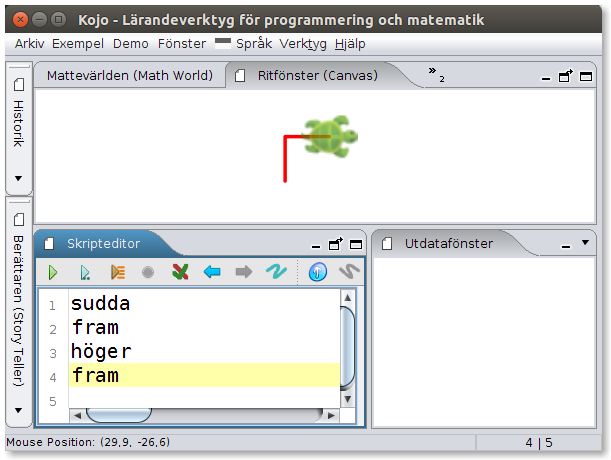
\includegraphics[width=0.7\textwidth]{../img/kojo}
\end{figure}
\pause position, rikting, pennfärg, pennbredd, penna uppe/nere, fyllfärg
\end{Slide} 

\begin{Slide}{Lata variabler och fördröjd evaluering} 
Med nyckelordet \code{lazy} före \code{val} skapas en s.k. ''lat'' \Eng{lazy} variabel.
\begin{REPL}
scala> val striktVektor = Vector.fill(1000000)(math.random)
striktVektor: scala.collection.immutable.Vector[Double] = 
 Vector(0.7583305221813246, 0.9016192590993339, 0.770022134260162, 0.15667718184929746, ...
 
scala> lazy val latVektor = Vector.fill(1000000)(math.random)
latVektor: scala.collection.immutable.Vector[Double] = <lazy>

scala> latVektor
res0: scala.collection.immutable.Vector[Double] = 
  Vector(0.5391685014341797, 0.14759775960530275, 0.722606095900537, 0.9025572787055386, ... 
\end{REPL}

En \code {lazy val} initialiseras \Alert{inte} vid deklarationen utan när den \Alert{refereras första gången}. Yttrycket som anges i deklarationen evalueras med s.k. \Emph{fördröjd evaluering} (även ''lat'' evaluering). 
\end{Slide} 

\begin{Slide}{Vad är egentligen skillnaden mellan \texttt{val}, \texttt{var}, \texttt{def} och \texttt{lazy val}?} 
\begin{Code}[basicstyle=\ttfamily\fontsize{8}{11}\selectfont]
object slump {
  val förAlltidSammaReferens  = math.random
  var kanÄndrasMedTilldelning = math.random
  def evaluerasVidVarjeAnrop  = math.random
  lazy val fördröjdInit       = Vector.fill(1000000)(math.random)
}
\end{Code}
\vspace{1em}\pause
Lat evaluering är en viktig princip inom funktionsprogrammering som möjliggör effektiva, oföränderliga datastrukturer där element allokeras först när de behövs. \\
\href{https://en.wikipedia.org/wiki/Lazy_evaluation}{en.wikipedia.org/wiki/Lazy\_evaluation}
\end{Slide} 


\Subsection{Funktioner är objekt}

\begin{Slide}{Programmeringsparadigm}
\href{https://en.wikipedia.org/wiki/Programming_paradigm}{en.wikipedia.org/wiki/Programming\_paradigm}:
\begin{itemize}
\item \Emph{Imperativ programmering}: programmet är uppbyggt av sekvenser av olika satser som läser och \Alert{ändrar} tillstånd
\item \Emph{Objektorienterad programmering}: en sorts imperativ programmering där programmet består av objekt som kapslar in tillstånd och erbjuder operationer som läser och \Alert{ändrar} tillstånd.
\item \Emph{Funktionsprogrammering}: programmet är uppbyggt av samverkande (matematiska) funktioner som \Alert{undviker} föränderlig data och tillståndsändringar. Oföränderliga datastrukturer skapar effektiva program i kombination med lat evaluering och rekursion. 
\end{itemize}
\end{Slide} 


\begin{Slide}{Funktioner är äkta objekt i Scala}
Scala visar hur man kan \Alert{förena} \Eng{unify} \\ \Emph{objekt-orientering} och \Emph{funktionsprogrammering}: \\\vspace{0.5em}

\textbf{\Large En funktion är ett objekt av funktionstyp\\ som har en \code{apply}-metod.}
\pause
\begin{REPLnonum}
scala> object öka extends (Int => Int) { 
         def apply(x: Int) = x + 1 
       }


scala> öka(1)
res0: Int = 2

scala> öka.   // tryck TAB
andThen   apply   compose   toString
\end{REPLnonum}
Mer om \code{extends} senare i kursen... %extends (Int => Int skrivs om till Function1[Int, Int]
\end{Slide} 


\Subsection{Rekursion}
\begin{Slide}{Rekursiva funktioner}
\begin{itemize}
\item Funktioner som \Alert{anropar sig själv} kallas \Emph{rekursiva}.


\begin{REPLnonum}
scala> def fakultet(n: Int): Int = 
         if (n < 2) 1 else n * fakultet(n - 1)

scala> fakultet(5)
res0: Int = 120
\end{REPLnonum}

\item För varje nytt anrop läggs en ny aktiveringspost på stacken. 

\item I aktiveringsposten sparas varje returvärde som gör att \code{5 * (4 * (3 * (2 * 1)))} kan beräknas. 

\item Rekrusionen avbryts när man når \Emph{basfallet}, här \code{n < 0}

\item En rekursiv funktion \Alert{måste} ha en returtyp.

\end{itemize}

\end{Slide} 

\begin{Slide}{Loopa med rekursion}
\begin{Code}
def gissaTalet(max: Int): Unit = {
  def gissat = io.StdIn.readLine(s"Gissa talet mellan [1, $max]: ").toInt 
  val hemlis = (math.random * max + 1).toInt
  def skrivLedtrådOmEjRätt(gissning: Int): Unit = 
    if (gissning > hemlis) println(s"$gissning är för stort :(") 
    else if (gissning < hemlis) println(s"$gissning är för litet :(")
  def ärRätt(gissning: Int): Boolean = { 
    skrivLedtrådOmEjRätt(gissning)
    gissning == hemlis
  }
  def loop(n: Int = 1): Int = if (ärRätt(gissat)) n else loop(n + 1)
  
  println(s"Du hittade talet $hemlis på ${loop()} gissningar :)")
}
\end{Code}
\end{Slide} 


\begin{Slide}{Rekursiva datastrukturer}

\begin{itemize}
\item Datastrukturena Lista och Träd är exempel på datastrukturer som passar bra ihop med rekursion. 
\item Båda dessa datastrukturer kan beskrivas rekursivt:
\begin{itemize}
\item En lista består av ett huvud och en lista, som i sin tur består av ett huvud och en lista, som i sin tur...
\item Ett träd består av grenar till träd som i sin tur består av grenar till träd som i sin tur, ...
\end{itemize}
\item Dessa datastrukturer bearbetas med fördel med rekursiva algoritmer.
\item I denna kursen ingår rekursion endast ''för kännedom'': \\ du ska veta vad det är och kunna skapa en enkel rekursiv funktion, t.ex. fakultets-beräkning. Du kommer jobba mer med rekursion och rekursiva datastrukturer i fortsättningskursen.
\end{itemize}
\end{Slide} 

\Subsection{SimpleWindow}
\begin{Slide}{Färdiga, enkla funktioner för att rita finns i klassen \texttt{cslib.window.SimpleWindow}}
På labben ska du använda \code{cslib.window.SimpleWindow}
\begin{itemize}
\item Paketet \code{cslib} innehåller paketet \code{window} som innehåller Java-klassen \code{SimpleWindow}.
%\item En \Emph{klass} är en ''mall'' för att göra \Emph{objekt}. 
\item Med \code{SimpleWindow} kan man skapa ritfönster. 
%\item När man skapar ett objekt från en klass använder man nyckelordet \code{new}.
\item Ladda ner \url{http://cs.lth.se/pgk/cslib} och lägg sedan jar-filen den katalog där du startar REPL med: \code{scala -cp cslib.jar}
\end{itemize}
\pause
\begin{REPLnonum}
$ scala -cp cslib.jar
scala> val w = new SimpleWindow(200,200,"hejsan")  
\end{REPLnonum}
\pause Studera dokumentationen för \code{cslib.window.SimpleWindow} här: \url{http://cs.lth.se/pgk/api/}
\end{Slide} 



\Subsection{Veckans övning och laboration}


\begin{Slide}{Övning \texttt{functions}}\SlideFontTiny
\setlength{\leftmargini}{0pt}
\begin{itemize}
%!TEX encoding = UTF-8 Unicode
%!TEX root = ../compendium2.tex

\item Kunna skapa och använda funktioner med en eller flera parametrar, default-argument, namngivna argument, och uppdelad parameterlista.
\item Kunna använda funktioner som äkta värden.
\item Kunna skapa och använda anonyma funktioner (s.k. lambda-funktioner).
\item Kunna applicera en funktion på element i en samling.
\item Förstå skillnader och likheter mellan en funktion och en procedur.
\item Förstå skillnader och likheter mellan en värde-anrop och namnanrop.
\item Kunna skapa en procedur i form av en enkel kontrollstruktur med fördröjd evaluering av ett block.
\item Kunna skapa och använda objekt som moduler.
\item Förstå skillnaden mellan äkta funktioner och funktioner med sidoeffekter.
\item Kunna skapa och använda variabler med fördröjd initialisering och förstå när de är användbara.
\item Kunna förklara hur nästlade funktionsanrop fungerar med hjälp av begreppet aktiveringspost.
\item Kunna skapa och använda lokala funktioner, samt förstå nyttan med lokala funktioner.
\item Känna till att funktioner är objekt med en \code{apply}-metod.
\item Känna till stegade funktioner och kunna använda partiellt applicerade argument.
\item Känna till rekursion och kunna förklara hur rekursiva funktioner fungerar.
%\item Känna till svansrekursion och att svansrekursiva funktioner kan optimeras till loopar.

\end{itemize}
\end{Slide} 


\begin{Slide}{Lab \texttt{blockmole}}%\SlideFontTiny
%\setlength{\leftmargini}{0pt}
\begin{itemize}
%!TEX encoding = UTF-8 Unicode
%!TEX root = ../compendium.tex

\item Kunna kompilera Scalaprogram med \texttt{scalac}.
\item Kunna köra Scalaprogram med \texttt{scala}.
\item Kunna definiera och anropa funktioner.
\item Kunna använda och förstå default-argument.
\item Kunna ange argument med parameternamn.
\item Kunna definiera objekt med medlemmar.
\item Förstå kvalificerade namn och import.
\item Förstå synlighet och skuggning.

\end{itemize}

\end{Slide} 



\Lecture{4}{Datastrukturer}
%!TEX encoding = UTF-8 Unicode
%!TEX root = ../lect-week04.tex

\ifkompendium\else

\begin{Slide}{Denna vecka: Fatta datastrukturer}
\begin{itemize}
\item Läs teori
\item Gör övning \code{data}
\item Gör lab \code{???}
\end{itemize}
\end{Slide}

\fi

%%%

\begin{Slide}{Olika sätt att skapa datastrukturer}
\begin{itemize}
\item Tupler
  \begin{itemize}
  \item samla $n$ st datavärden i element \Emph{\code{_1}}, \Emph{\code{_2}}, ...  \code{_}$n$
  \item elementen kan vara av \Alert{olika} typ
  \end{itemize}
\item Klasser   
  \begin{itemize}
  \item samlar data i \Emph{attribut} med (väl valda!) namn
  \item attributen kan vara av \Alert{olika} typ
  \item definierar även metoder som använder attributen (operationer på data)
  \end{itemize}

\item Samlingar 
  \begin{itemize}
  \item speciella klasser som samlar data i element av \Alert{samma} typ
  \item finns ofta \emph{många} färdiga \Emph{bra-att-ha-metoder} 
  \end{itemize}
\end{itemize}
\end{Slide}

\ifkompendium\else

\begin{Slide}{Vad är en tupel?}
\code{("hej", 42, math.Pi)} är en 3-tupel med typ: \code{(String, Int, Double)}
\end{Slide}

\fi


\begin{Slide}{Hierarki av samlingar i scala.collection}
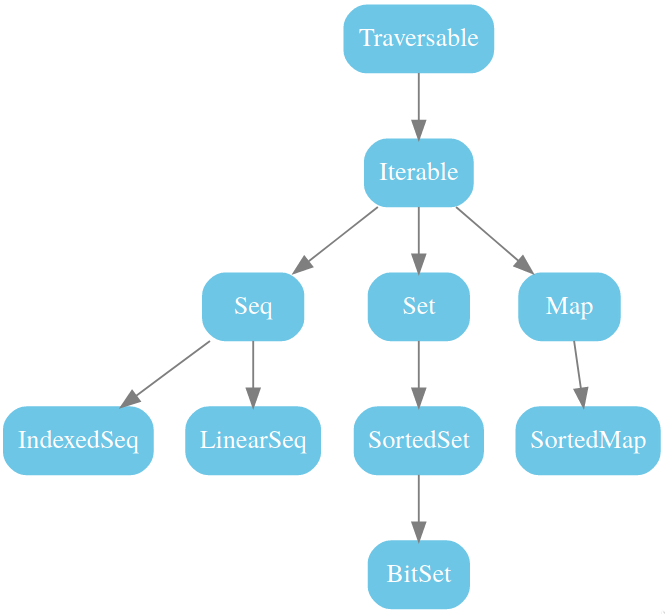
\includegraphics[width=1.0\textwidth]{../img/collection/collection-traits}
\end{Slide}

\ifkompendium
\noindent Läs mer om Scalas samlingar här: \\ 
\url{http://docs.scala-lang.org/overviews/collections/overview}
\else\fi

\ifkompendium\else

\begin{Slide}{scala.collection.immutable}
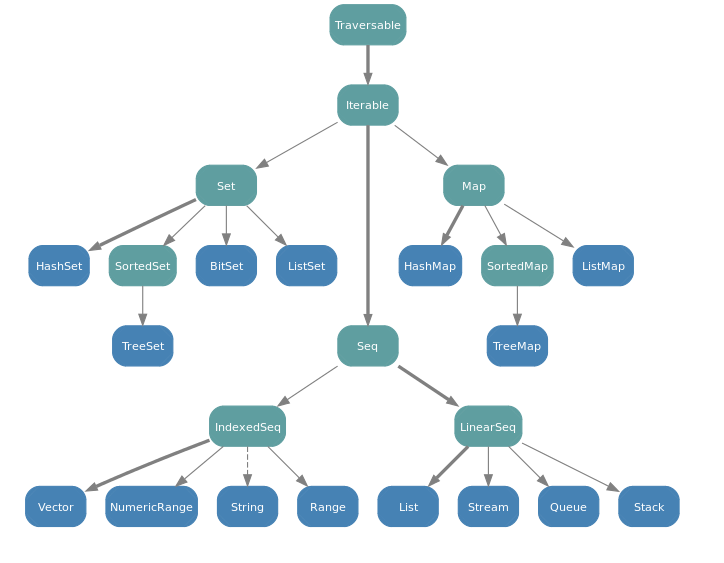
\includegraphics[width=0.82\textwidth]{../img/collection/collection-immutable}
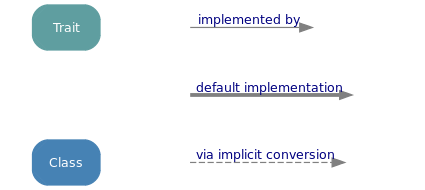
\includegraphics[width=0.33\textwidth]{../img/collection/collection-legend}
\end{Slide}

\begin{Slide}{scala.collection.mutable}
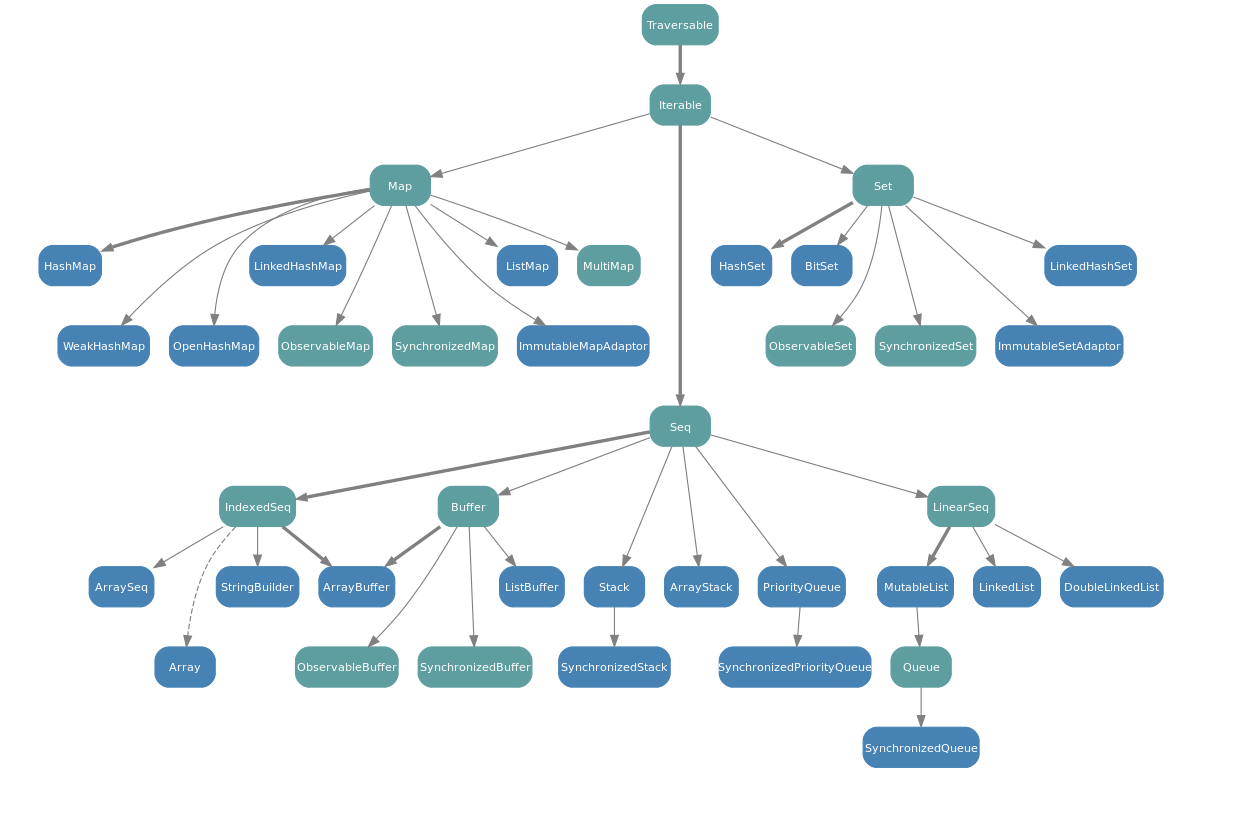
\includegraphics[width=1.05\textwidth]{../img/collection/collection-mutable}
\end{Slide}
\fi


% ??? Berätta om javafx.util.pair
% http://stackoverflow.com/questions/521171/a-java-collection-of-value-pairs-tuples




%!TEX encoding = UTF-8 Unicode
%!TEX root = ../lect-week04.tex

\ifkompendium\else

\Subsection{Tupler}

\begin{Slide}{Vad är en tupel?}\SlideFontSmall

\begin{itemize}
\item En tupel samlar $n$ st objekt i en enkel struktur, med koncis syntax.
  \item Elementen kan vara av \Alert{olika} typ.

\item 
\code{("hej", 42, math.Pi)} är en \Emph{3-tupel} av typen: \code{(String, Int, Double)}

\item Du kan komma åt de enskilda elementen med \Emph{\code{_1}}, \Emph{\code{_2}}, ...  \code{_}$n$

\begin{REPL}
scala> val t = ("hej", 42, math.Pi)
t: (String, Int, Double) = (hej,42,3.141592653589793)

scala> t._1
res0: String = hej

scala> t._2
res1: Int = 42
\end{REPL}

\item Tupler är praktiska när man inte vill ta det lite större arbetet att skapa en egen klass.
(Men med klasser kan man göra mycket mer än med tupler.)

\item I Scala kan du skapa tupler upp till en storlek av 22 element. 
\\ (Behöver du fler element, använd i stället en samling, t.ex. \code{Vector}.)

\end{itemize}

\end{Slide}




\begin{Slide}{Tupler som parametrar och returvärde.}\SlideFontSmall

\begin{itemize}

\item Tupler är smidiga när man på ett enkelt och typsäkert sätt vill låta en funktion \Emph{returnera mer än ett värde}.

\begin{REPL}
scala> def längd(p: (Double, Double)) = math.hypot(p._1, p._2)

scala> def vinkel(p: (Double, Double)) = math.atan2(p._1, p._2) 

scala> def polär(p: (Double, Double)) = (längd(p), vinkel(p))

scala> polär((3,4))
res2: (Double, Double) = (5.0,0.6435011087932844)

\end{REPL}
\vspace{0.5em}
\item Om typerna passar kan man skippa dubbla parenteser vid \Emph{ensamt tupel-argument}:
\begin{REPL}
scala> polär(3,4)
res3: (Double, Double) = (5.0,0.6435011087932844)
\end{REPL}
\item[] {\SlideFontTiny\href{https://sv.wikipedia.org/wiki/Pol\%C3\%A4ra_koordinater}{https://sv.wikipedia.org/wiki/Polära\_koordinater}}


\end{itemize}
\end{Slide}

\begin{Slide}{Ett smidigt sätt att skapa 2-tupler med metoden \texttt{->}}
Det finns en metod vid namn \code{->} som kan användas på objekt av \Alert{godtycklig} typ för att \Emph{skapa par}:

\vspace{0.8em}
\begin{REPL}
scala> ("Ålder", 42)
res0: (String, Int) = (Ålder,42)

scala> "Ålder".->(42)
res1: (String, Int) = (Ålder,42)

scala> "Ålder" -> 42
res2: (String, Int) = (Ålder,42)

scala> Vector("Ålder" -> 42, "Längd" -> 178, "Vikt" -> 65) 
res3: scala.collection.immutable.Vector[(String, Int)] = 
        Vector((Ålder,42), (Längd,178), (Vikt, 65))


\end{REPL}



\end{Slide}


\fi



% ??? Berätta om javafx.util.pair
% http://stackoverflow.com/questions/521171/a-java-collection-of-value-pairs-tuples




%!TEX encoding = UTF-8 Unicode
%!TEX root = ../lect-week04.tex

\ifkompendium\else

\Subsection{Klasser}

\begin{Slide}{Vad är en klass?}\SlideFontSmall
Vi har tidigare deklarerat \Emph{singelobjekt} som bara finns i \Alert{en} \Emph{instans}:
\begin{REPLnonum}
scala> object Björn { var ålder = 49; val längd = 178 }
\end{REPLnonum}

Med en \Emph{klass} kan man skapa \Alert{godtyckligt många} \Emph{instanser av klassen} med hjälp av nyckelordet \code{new} följt av klassens namn:

\begin{REPLnonum}
scala> class Person { var ålder = 0; var längd = 0 }

scala> val björn = new Person
björn: Person = Person@7ae75ba6

scala> björn.ålder = 49

scala> björn.längd = 178
\end{REPLnonum}

\begin{itemize}

\item En klass kan ha \Emph{medlemmar} (i likhet med singelobjekt). 

\item Funktioner som är medlemmar kallas \Emph{metoder}.

\item Variabler som är medlemmar kallas \Emph{attribut}.


\end{itemize}

\end{Slide}


\begin{Slide}{Vid \texttt{new} allokeras plats i minnet för objektet}
\begin{REPLnonum}
scala> class Person { var ålder = 0; var längd = 0 }

scala> val björn = new Person
björn: Person = Person@7ae75ba6
\end{REPLnonum}

\begin{tikzpicture}[font=\large\sffamily]
\matrix [matrix of nodes, row sep=0, column 2/.style={nodes={rectangle,draw,minimum width=0.8cm}}] (mat) 
{
\texttt{björn}   &  \makebox(10,10){ }\\
};
\node[cloud, cloud puffs=13.0, cloud ignores aspect, minimum width=2cm, minimum height=3.8cm,
 align=center, draw] (x) at (5.8cm, -1.5cm) { 
 \begin{tabular}{r l}
 \multicolumn{2}{c}{\ttfamily\itshape Person@7ae75ba6}\\ \\
 \texttt{ålder} & \fbox{~0~} \\
 \texttt{längd} & \fbox{~0~}\\
 \end{tabular}
 };
\filldraw[black] (0.75cm,0.0cm) circle (3pt) node[] (ref) {};
\draw [arrow, line width=0.7mm] (ref) -- (x);
% \node[cloud, cloud puffs=15.7, cloud ignores aspect, %minimum width=5cm, minimum height=2cm,
% align=center, draw] (g2) at (5cm, -2cm) {Gurka-\\objekt};
% \filldraw[black] (0.4cm,-0.4cm) circle (3pt) node[] (g2ref) {};
% \draw [arrow] (g2ref) -- (g2);
\end{tikzpicture}
{\SlideFontTiny{\ttfamily\itshape Person@7ae75ba6} är en unik idenfierare för instansen, så att JVM hittar den i heapen.}
\end{Slide}



\begin{Slide}{Med punktnotation kan förändringsbara variabler tilldelas nya värden och objektets tillstånd uppdateras.}
\begin{REPLnonum}
scala> björn.ålder = 49
scala> björn.längd = 178
\end{REPLnonum}

\begin{tikzpicture}[font=\large\sffamily]
\matrix [matrix of nodes, row sep=0, column 2/.style={nodes={rectangle,draw,minimum width=0.8cm}}] (mat) 
{
\texttt{björn}   &  \makebox(10,10){ }\\
};
\node[cloud, cloud puffs=13.0, cloud ignores aspect, minimum width=2cm, minimum height=3.8cm,
 align=center, draw] (x) at (5.8cm, -1.5cm) { 
 \begin{tabular}{r l}
 \multicolumn{2}{c}{\ttfamily\itshape Person@7ae75ba6}\\ \\
 \texttt{ålder} & \fbox{~49~~} \\
 \texttt{längd} & \fbox{~178}\\
 \end{tabular}
 };
\filldraw[black] (0.75cm,0.0cm) circle (3pt) node[] (ref) {};
\draw [arrow, line width=0.7mm] (ref) -- (x);
% \node[cloud, cloud puffs=15.7, cloud ignores aspect, %minimum width=5cm, minimum height=2cm,
% align=center, draw] (g2) at (5cm, -2cm) {Gurka-\\objekt};
% \filldraw[black] (0.4cm,-0.4cm) circle (3pt) node[] (g2ref) {};
% \draw [arrow] (g2ref) -- (g2);
\end{tikzpicture}
\end{Slide}





\begin{Slide}{En klass kan ha parametrar som initialiserar attribut}
\begin{itemize}
\item Med en parameterlista efter klassnamnet får man en så kallad \Emph{primärkonstruktor} för initialisering av attribut. 
\item Argumenten för initialiseringen ges vid \code{new}.
\begin{REPLnonum}
scala> class Person(var ålder: Int, var längd: Int)

scala> val björn = new Person(49, 178)
björn: Person = Person@354baab2

scala> println(s"Björn är ${björn.ålder} år gammal.")
Björn är 49 år gammal.

scala> björn.ålder = 18

scala> println(s"Björn är ${björn.ålder} år gammal.")
Björn är 18 år gammal.
\end{REPLnonum}
\end{itemize}
\end{Slide}




\begin{Slide}{En klass kan ha privata medlemmar}
Med \code{private} blir en medlem \Emph{privat}: access utifrån \Alert{medges ej}.

\vspace{0.1em}
\begin{REPL}
scala> class Person(private var minÅlder: Int, private var minLängd: Int){
         def ålder = minÅlder
       }

scala> val björn = new Person(42, 178)
björn: Person = Person@4b682e71

scala> println(s"Björn är ${björn.ålder} år gammal.")
Björn är 42 år gammal.

scala> björn.minÅlder = 18
error: variable minÅlder in class Person cannot be accessed in Person

scala> björn.längd
error: value längd is not a member of Person
\end{REPL}
Med \code{private} kan man förhindra tokiga förändringar.
\end{Slide}


\begin{Slide}{Privata förändringsbara attribut och publika metoder}
\begin{Code}
class Människa(val födelseLängd: Double, val födelseVikt: Double){
  private var minLängd = födelseLängd
  private var minVikt  = födelseVikt
  private var ålder    = 0
    
  def längd = minLängd  // en sådan här metod kallas "getter"
  def vikt  = minVikt   // vi förhindrar attributändring "utanför" klassen
    
  val slutaVäxaÅlder      = 18
  val tillväxtfaktorLängd = 0.00001
  val tillväxtfaktorVikt  = 0.0002

  def ät(mat: Double): Unit = {
    if (ålder < slutaVäxaÅlder) minLängd += tillväxtfaktorLängd * mat
    minVikt += tillväxtfaktorVikt * mat
  }
  
  def fyllÅr: Unit = ålder += 1
  
  def tillstånd: String = s"Tillstånd: $minVikt kg, $minLängd cm, $ålder år"
}
\end{Code}
\end{Slide}

\begin{Slide}{Tillstånd kan förändras indirekt genom metodanrop}
\begin{REPL}
scala> val björn = new Människa(födelseVikt=3.5, födelseLängd=52.1)
björn: Människa = Människa3e52

scala> björn.tillstånd
res0: String = Tillstånd: 3.5 kg, 52.1 cm, 0 år

scala> for (i <- 1 to 42) björn.fyllÅr

scala> björn.tillstånd
res2: String = Tillstånd: 3.5 kg, 52.1 cm, 42 år

scala> björn.ät(mat=5000)

scala> björn.tillstånd
res3: String = Tillstånd: 4.5 kg, 52.1 cm, 42 år
\end{REPL}
\end{Slide}



\begin{Slide}{Metoden \texttt{isInstanceOf} och rot-typen \texttt{Any}}
\SlideFontSmall\vspace{-0.5em}
\begin{multicols}{2}

\begin{REPL}
scala> class X(val i: Int) 

scala> val a = new X(42)
a: X = X@117b2cc6

scala> a.isInstanceOf[X]
res0: Boolean = true

scala> val b = new X(42)
b: X = X@61ab6521

scala> b.isInstanceOf[X]
res1: Boolean = true

scala> a == b
res2: Boolean = false

scala> a.i == b.i
res3: Boolean = true

\end{REPL}

\columnbreak


\begin{itemize}\SlideFontTiny

\item Ett objekt skapat med \code{new X} är en instans av \Emph{typen} \code{X}. 

\item Detta kan testas med metoden \code{isInstanceOf[X]: Boolean}

\pause

\item Typen \Emph{\texttt{Any}} är sypertyp till \Alert{alla} typer och kallas för \Emph{rot-typ} i Scalas  typhierarki. 

\begin{REPL}
scala> a.isInstanceOf[Any]
res4: Boolean = true

scala> b.isInstanceOf[Any]
res5: Boolean = true

scala> 42.isInstanceOf[Any]
res6: Boolean = true

\end{REPL}
\item Se quickref sid 4. (Mer i w07.) 
\item I klassen \href{http://www.scala-lang.org/api/current/#scala.Any}{\code{Any}} finns bl.a. \code{toString}
\end{itemize}
%{\SlideFontTiny \hfill(se quickref sid 4, mer om detta i w07)}
\end{multicols}
\end{Slide}



\begin{Slide}{Överskugga \texttt{toString}}
Alla objekt får automatiskt en metod \code{toString} som ger en sträng med objektets unika identifierare, här \texttt{Gurka@3830f1c0}:
\begin{REPL}
scala> class Gurka(val vikt: Int) 

scala> val g = new Gurka(42)
g: Gurka = Gurka@3830f1c0

scala> g.toString
res0: String = Gurka@3830f1c0
\end{REPL}
Man kan \Emph{överskugga} den automatiska \code{toString}  med en \Alert{egen implementation}. Observera nyckerordet \code{override}.
\begin{REPL}
scala> class Tomat(val vikt: Int){override def toString = s"Tomat($vikt g)"} 

scala> val t = new Tomat(142)
t: Tomat = Tomat(142 g)

scala> t.toString
res1: String = Tomat(142 g)

\end{REPL}
\end{Slide}





\begin{Slide}{Objektfabrik i kompanjonsobjekt}%\SlideFontSmall
\begin{itemize}
\item Om det finns ett objekt i samma kodfil med samma namn som klassen blir det objektet ett s.k.  \Emph{kompanjonsobjekt} \Eng{companion object}.

\item Ett kompanjonsobjekt får \Alert{accessa privata medelmmar} i den klass till vilken objektet är kompanjon.

\item Kompanjonsobjekt är en bra plats för s.k. \Emph{fabriksmetoder} som skapar instanser. Då slipper vi skriva \code{new}.
\begin{REPL}
scala> :paste   // måste skrivas tillsammans annars ingen kompanjon

class Broccoli(var vikt: Int) 

object Broccoli {
  def apply(vikt: Int) = new Broccoli(vikt)
}

scala> val b = Broccoli(420)
b: Broccoli = Broccoli@32e8d5a4
\end{REPL}

\end{itemize}
\end{Slide}


\begin{Slide}{Kompanjonsobjekt kan accessa privata medlemmar}%\SlideFontSmall
\begin{Code}
class Gurka(startVikt: Double) {
  private var vikt = startVikt
  def ät(tugga: Int): Unit = if (vikt > tugga) vikt -= tugga else vikt = 0 
  override def toString = s"Gurka($vikt)"
}
object Gurka {
  private var totalVikt = 0.0
  def apply(): Gurka = {
    val g = new Gurka(math.random * 0.42 + 0.1)
    totalVikt += g.vikt  // hade blivit kompileringsfel om ej vore kompanjon
    g
  }
  def rapport: String = s"Du har skapat ${totalVikt.toInt} kg gurka." 
}
\end{Code}
\pause
\begin{REPL}
scala> val gs = Vector.fill(1000)(Gurka())
gs: scala.collection.immutable.Vector[Gurka] = 
  Vector(Gurka(0.49018400799506734), Gurka(0.2462822679714138), Gurka(0.17391397513818804), Gurka(0.5146514905924656), Gurka(0.47077333689159606)

scala> println(Gurka.rapport)
Du har skapat 305 kg gurka.

\end{REPL}

\end{Slide}






\begin{Slide}{Förändringsbara och oföränderliga objekt}
Ett \Emph{oföränderligt objekt} där nya instanser skapas i stället för tillståndsändring ''på plats''.
\begin{Code}
class Point(val x: Int, val y: Int) {
  def moved(dx: Int, dy: Int): Point = new Point(x + dx, y + dy)

  override def toString: String = s"Point($x, $y)"
}
\end{Code}

Ett \Alert{förändringsbart} objekt där \Alert{tillståndet uppdateras}.
\begin{Code}
class MutablePoint(private var x: Int, private var y: Int) {
  def move(dx: Int, dy: Int): Unit = {x += dx; y += dy}  // Mutation!!!

  override def toString: String = s"MutablePoint($x, $y)"
}
\end{Code}
\end{Slide}


\begin{Slide}{Oföränderliga objekt}

\begin{minipage}{0.5\textwidth}
\begin{REPL}
scala> var p1 = new Point(3, 4)
p1: Point = Point(3, 4)

scala> val p2 = p1.moved(2, 3)
p2: Point = Point(5, 7)

scala> println(p1)
Point(3, 4)

scala> p1 = new Point(0, 0)
p1: Point = Point(0, 0)
\end{REPL}
\end{minipage}
\pause\begin{minipage}{0.49\textwidth}
{\SlideFontSmall \hfill Minnessituationen efter rad 7:}

\vspace{1em}
\begin{tikzpicture}[font=\SlideFontSmall\sffamily,scale=0.75, every node/.style={scale=0.75}]
\matrix [matrix of nodes, row sep=0, column 2/.style={nodes={rectangle,draw,minimum width=0.6cm}}] (mat) 
{
\texttt{p1}   &  \makebox(7,7){ }\\
};
\node[cloud, cloud puffs=13.0, cloud ignores aspect, minimum width=2cm, minimum height=1cm,
 align=center, draw] (x) at (3cm, -0.0cm) { 
 \begin{tabular}{r l}
 \texttt{x} & \fbox{~3~} \\
 \texttt{y} & \fbox{~4~}\\
 \end{tabular}
 };
\filldraw[black] (0.25cm,0.0cm) circle (3pt) node[] (ref) {};
\draw [arrow, line width=0.5mm] (ref) -- (x);
\end{tikzpicture}

\begin{tikzpicture}[font=\SlideFontSmall\sffamily,scale=0.75, every node/.style={scale=0.75}]
\matrix [matrix of nodes, row sep=0, column 2/.style={nodes={rectangle,draw,minimum width=0.6cm}}] (mat) 
{
\texttt{p2}   &  \makebox(7,7){ }\\
};
\node[cloud, cloud puffs=13.0, cloud ignores aspect, minimum width=2cm, minimum height=1cm,
 align=center, draw] (x) at (3cm, -0.0cm) { 
 \begin{tabular}{r l}
 \texttt{x} & \fbox{~5~} \\
 \texttt{y} & \fbox{~7~}\\
 \end{tabular}
 };
\filldraw[black] (0.25cm,0.0cm) circle (3pt) node[] (ref) {};
\draw [arrow, line width=0.5mm] (ref) -- (x);
\end{tikzpicture}

\end{minipage}

\end{Slide}



\begin{Slide}{Oföränderliga objekt}

\begin{minipage}{0.5\textwidth}
\begin{REPL}
scala> var p1 = new Point(3, 4)
p1: Point = Point(3, 4)

scala> val p2 = p1.moved(2, 3)
p2: Point = Point(5, 7)

scala> println(p1)
Point(3, 4)

scala> p1 = new Point(0, 0)
p1: Point = Point(0, 0)
\end{REPL}
\end{minipage}
\begin{minipage}{0.49\textwidth}
{\SlideFontSmall \hfill Minnessituationen efter rad 10:}

\vspace{1em}
\begin{tikzpicture}[font=\SlideFontSmall\sffamily,scale=0.75, every node/.style={scale=0.75}]
\node[cloud, cloud puffs=13.0, cloud ignores aspect, minimum width=2cm, minimum height=1cm,
 align=center, draw] (x) at (3cm, 2.0cm) { 
 \begin{tabular}{r l}
 \texttt{x} & \fbox{~3~} \\
 \texttt{y} & \fbox{~4~}\\
 \end{tabular}
 };
 
 \node[left of=x, text width=2.5cm,align=right] (text) at (1,2) {kommer att raderas av skräpsamlaren:};
\end{tikzpicture}

\begin{tikzpicture}[font=\SlideFontSmall\sffamily,scale=0.75, every node/.style={scale=0.75}]
\matrix [matrix of nodes, row sep=0, column 2/.style={nodes={rectangle,draw,minimum width=0.6cm}}] (mat) 
{
\texttt{p2}   &  \makebox(7,7){ }\\
};
\node[cloud, cloud puffs=13.0, cloud ignores aspect, minimum width=2cm, minimum height=1cm,
 align=center, draw] (x) at (3cm, -0.0cm) { 
 \begin{tabular}{r l}
 \texttt{x} & \fbox{~5~} \\
 \texttt{y} & \fbox{~7~}\\
 \end{tabular}
 };
\filldraw[black] (0.25cm,0.0cm) circle (3pt) node[] (ref) {};
\draw [arrow, line width=0.5mm] (ref) -- (x);
\end{tikzpicture}

\begin{tikzpicture}[font=\SlideFontSmall\sffamily,scale=0.75, every node/.style={scale=0.75}]
\matrix [matrix of nodes, row sep=0, column 2/.style={nodes={rectangle,draw,minimum width=0.6cm}}] (mat) 
{
\texttt{p1}   &  \makebox(7,7){ }\\
};
\node[cloud, cloud puffs=13.0, cloud ignores aspect, minimum width=2cm, minimum height=1cm,
 align=center, draw] (x) at (3cm, -0.0cm) { 
 \begin{tabular}{r l}
 \texttt{x} & \fbox{~0~} \\
 \texttt{y} & \fbox{~0~}\\
 \end{tabular}
 };
\filldraw[black] (0.25cm,0.0cm) circle (3pt) node[] (ref) {};
\draw [arrow, line width=0.5mm] (ref) -- (x);
\end{tikzpicture}

\end{minipage}

\pause\vspace{1em}Vi kan \Emph{lugnt dela referenser} till vårt oföränderliga objekt eftersom det \Emph{aldrig} kommer att ändras.

\end{Slide}


\newcommand{\MutaVarning}{\vspace{2em}\Alert{Varning!} Vem som helst som har tillgång till en referens till ditt förändringsbara objekt kan \Alert{manipulera} det, vilket ibland ger överaskande och \Alert{problematiska} konsekvenser!}



\begin{Slide}{Förändringsbara objekt}

\begin{minipage}{0.5\textwidth}
\begin{REPL}
scala> val mp1 = new MutablePoint(3, 4)
mp1: MutablePoint = MutablePoint(3, 4)

scala> val mp2 = mp1
mp2: MutablePoint = MutablePoint(3, 4)

scala> mp1.move(2,3)

scala> println(mp2)
MutablePoint(5, 7)
\end{REPL}
\end{minipage}
\begin{minipage}{0.49\textwidth}
{\SlideFontSmall \hfill Minnessituationen efter rad 4:}

\vspace{1em}
\begin{tikzpicture}[font=\SlideFontSmall\sffamily,scale=0.75, every node/.style={scale=0.75}]
\matrix [matrix of nodes, row sep=0.5cm, column 2/.style={nodes={rectangle,draw,minimum width=0.6cm}}] (mat) 
{
\texttt{mp1}   &  \makebox(7,7){ }\\
\texttt{mp2}   &  \makebox(7,7){ }\\
};
\node[cloud, cloud puffs=13.0, cloud ignores aspect, minimum width=2cm, minimum height=1cm,
 align=center, draw] (x) at (3cm, -0.0cm) { 
 \begin{tabular}{r l}
 \texttt{x} & \fbox{~3~} \\
 \texttt{y} & \fbox{~4~}\\
 \end{tabular}
 };
\filldraw[black] (0.35cm,0.65cm) circle (3pt) node[] (ref1) {};
\draw [arrow, line width=0.5mm] (ref1) -- (x);

\filldraw[black] (0.35cm,-0.65cm) circle (3pt) node[] (ref2) {};
\draw [arrow, line width=0.5mm] (ref2) -- (x);


\end{tikzpicture}

\end{minipage}

\pause\MutaVarning
\end{Slide}




\begin{Slide}{Förändringsbara objekt}

\begin{minipage}{0.5\textwidth}
\begin{REPL}
scala> val mp1 = new MutablePoint(3, 4)
mp1: MutablePoint = MutablePoint(3, 4)

scala> val mp2 = mp1
mp2: MutablePoint = MutablePoint(3, 4)

scala> mp1.move(2,3)

scala> println(mp2)
MutablePoint(5, 7)
\end{REPL}
\end{minipage}
\begin{minipage}{0.49\textwidth}
{\SlideFontSmall \hfill Minnessituationen efter \Alert{rad 7}:}

\vspace{1em}
\begin{tikzpicture}[font=\SlideFontSmall\sffamily,scale=0.75, every node/.style={scale=0.75}]
\matrix [matrix of nodes, row sep=0.5cm, column 2/.style={nodes={rectangle,draw,minimum width=0.6cm}}] (mat) 
{
\texttt{mp1}   &  \makebox(7,7){ }\\
\texttt{mp2}   &  \makebox(7,7){ }\\
};
\node[cloud, cloud puffs=13.0, cloud ignores aspect, minimum width=2cm, minimum height=1cm,
 align=center, draw] (x) at (3cm, -0.0cm) { 
 \begin{tabular}{r l}
 \texttt{x} & \fbox{~5~} \\
 \texttt{y} & \fbox{~7~}\\
 \end{tabular}
 };
\filldraw[black] (0.35cm,0.65cm) circle (3pt) node[] (ref1) {};
\draw [arrow, line width=0.5mm] (ref1) -- (x);

\filldraw[black] (0.35cm,-0.65cm) circle (3pt) node[] (ref2) {};
\draw [arrow, line width=0.5mm] (ref2) -- (x);


\end{tikzpicture}

\end{minipage}

\MutaVarning
\end{Slide}





\Subsection{Case-klasser}

\begin{Slide}{Vad är en case-klass?}\SlideFontSmall
\setlength{\leftmargini}{0pt}
\begin{itemize}
\item En \code{case}-klass är ett smidigt sätt att skapa \Emph{oföränderliga objekt}.
\item Kompilatorn ger dig \Alert{en massa ''godis''} på köpet (ca 50-100 rader kod), inkl.:
\begin{itemize}\SlideFontTiny
\item klassparametrar blir automatiskt \code{val}-attribut, alltså \Emph{publika} och \Emph{oföränderliga},
\item en automatisk \Emph{\texttt{toString}} som visar klassparametrarnas värde, 
\item ett automatiskt \Emph{kompanjonsobjekt} med \Emph{fabriksmetod} så du slipper skriva \code{new},
\item automatiska metoden \Emph{\texttt{copy}} för att skapa kopior med andra attributvärden, m.m...
\item[] (Mer om detta i w06 \& w11, men är du nyfiken kolla på uppgift 2d) på sid 261.)
\end{itemize}

\pause
\item Det \Alert{enda} du behöver göra är att lägga till nyckelordet \code{case} före \code{class}...
\end{itemize}

\vspace{-0.5em}\begin{REPLnonum}
scala> case class Point(x: Int, y: Int)

scala> val p = Point(3, 5)
p: Point = Point(3,5)

scala> p.  // tryck TAB och se lite av allt case-klass-godis
scala> Point.  // tryck TAB och se ännu mer godis

scala> val p2 = p.copy(y= 30)
p2: Point = Point(3,30)
\end{REPLnonum}


\end{Slide}


\begin{Slide}{Exempel på case-klasser} 
\begin{Code}
case class Person(namn: String, ålder: Int) {
  def fyllerJämt: Boolean = ålder % 10 == 0
  def hyllning = if (fyllerJämt) "Extra grattis!" else "Vi gratulerar!"
  def ärLikaGammalSom(annan: Person) = ålder == annan.ålder
}

case class Point(x: Int = 0, y: Int = 0) {
  def distanceTo(other: Point) = math.hypot(x - other.x, y - other.y)
  def dx(d: Int): Point = copy(x + d, y)
  def dy(d: Int): Point = copy(y= y + d)  //namngivet arg. och defaultarg.
}
object Point { 
  def origin = new Point() 
}
\end{Code}

\begin{REPL}
scala> Point().dx(10).dy(10).dx(32)
res0: Point = Point(42,10)

scala> Point(3,4) distanceTo Point.origin
res1: Double = 5.0

\end{REPL}
\end{Slide}

\begin{Slide}{Synlighet av klassparametrar i klasser \& case-klasser}\SlideFontSmall
\code{private[this]} är \Alert{ännu} mer privat än \code{private} 
\begin{Code}
class Hemlis(private val hemlis: Int) {
  def ärSammaSom(annan: Hemlis) = hemlis == annan.hemlis   // Funkar!
}

class Hemligare(private[this] val hemlis: Int) {
  def ärSammaSom(annan: Hemligare) = hemlis == annan.hemlis //KOMPILERINGSFEL
}
\end{Code}
Vad händer om man inte skriver något? Olika för klass och case-klass:
\begin{Code}
class Hemligare(hemlis: Int) { // motsvarar private[this] val
  def ärSammaSom(annan: Hemligare) = hemlis == annan.hemlis //KOMPILERINGSFEL
}

case class InteHemlig(seMenInteRöra: Int) { // blir automatiskt val 
  def ärSammaSom(annan: InteHemlig): Boolean = 
    seMenInteRöra == annan.seMenInteRöra 
}

\end{Code}
\end{Slide}

\fi





%!TEX encoding = UTF-8 Unicode
%!TEX root = ../lect-week04.tex

\ifkompendium\else
\Subsection{Samlingar}

\begin{Slide}{Vad är en samling?}
En \Emph{samling} \Eng{collection} är en datastruktur som kan innehålla många element av \Alert{samma typ}.
\end{Slide}

\fi

\begin{Slide}{Hierarki av samlingar i scala.collection}
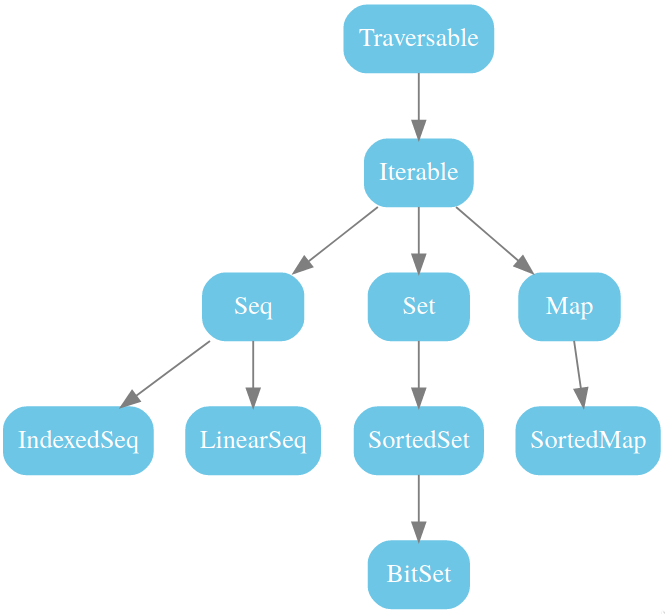
\includegraphics[width=1.0\textwidth]{../img/collection/collection-traits}
\end{Slide}

\noindent Läs mer om Scalas samlingar här: \\ 
\url{http://docs.scala-lang.org/overviews/collections/overview}

\ifkompendium\else

\begin{Slide}{scala.collection.immutable}
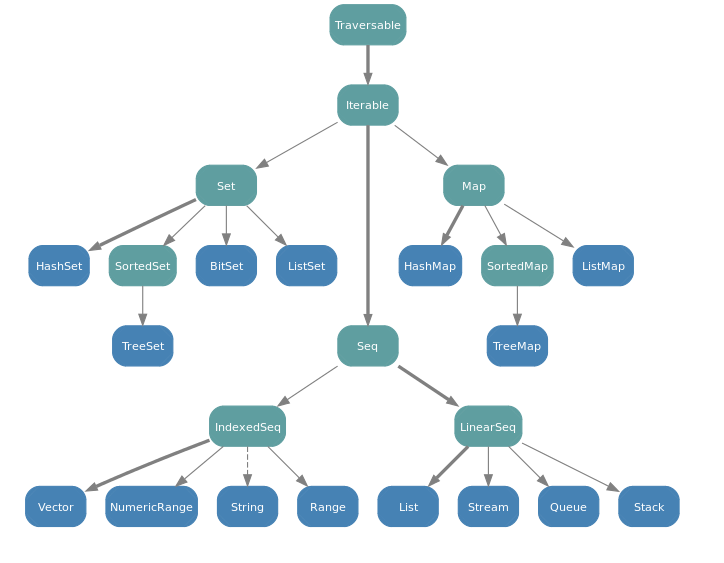
\includegraphics[width=0.82\textwidth]{../img/collection/collection-immutable}
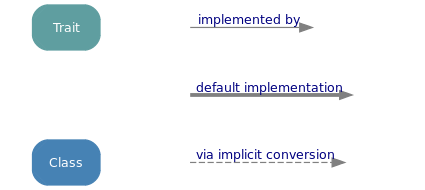
\includegraphics[width=0.33\textwidth]{../img/collection/collection-legend}
\end{Slide}

\begin{Slide}{scala.collection.mutable}
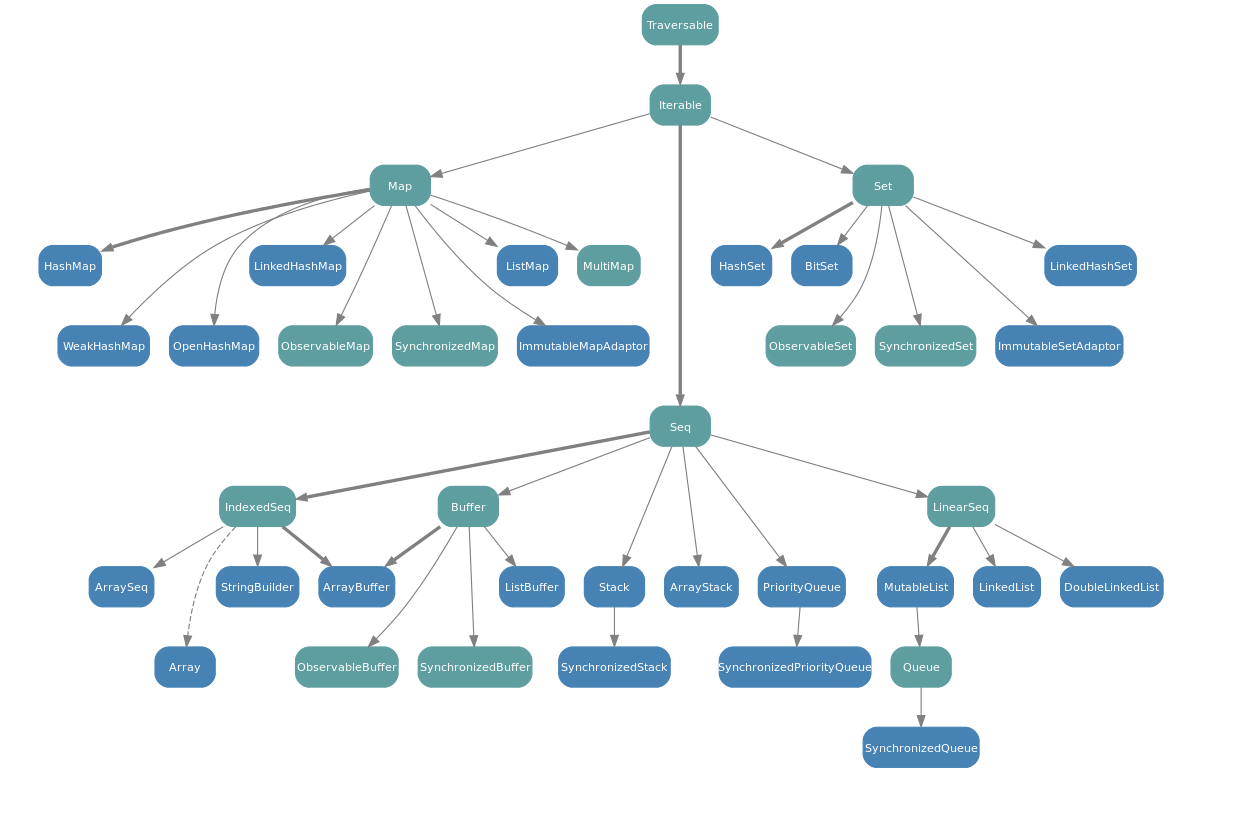
\includegraphics[width=1.05\textwidth]{../img/collection/collection-mutable}
\end{Slide}


\begin{Slide}{Vector eller List???}\SlideFontTiny
\url{http://stackoverflow.com/questions/6928327/when-should-i-choose-vector-in-scala}

''
\begin{itemize}
\item We only need to transform sequences by operations like map, filter, fold etc: basically it does not matter, we should program our algorithm generically and might even benefit from accepting parallel sequences. For sequential operations List is probably a bit faster. But you should benchmark it if you have to optimize.

\item We need a lot of random access and different updates, so we should use vector, list will be prohibitively slow.

\item We operate on lists in a classical functional way, building them by prepending and iterating by recursive decomposition: use list, vector will be slower by a factor 10-100 or more.

\item We have an performance critical algorithm that is basically imperative and does a lot of random access on a list, something like in place quick-sort: use an imperative data structure, e.g. ArrayBuffer, locally and copy your data from and to it.


\end{itemize}
\end{Slide}

\fi






%!TEX encoding = UTF-8 Unicode
%!TEX root = ../lect-week04.tex

\ifkompendium\else
\Subsection{Integrerad utvecklingsmiljö (IDE)}

\begin{Slide}{Välja IDE}
\end{Slide}

\begin{Slide}{Denna veckas övning: \texttt{data}}
\begin{itemize}\SlideFontTiny
%!TEX encoding = UTF-8 Unicode
%!TEX root = ../compendium.tex

\item Kunna skapa och använda tupler, som variabelvärden, parametrar och returvärden.

\item Förstå skillnaden mellan ett objekt och en klass och kunna förklara betydelsen av begreppet instans.

\item Kunna skapa och använda attribut som medlemmar i objekt och klasser och som som klassparametrar.

\item Beskriva innebörden av och syftet med att ett attribut är privat.

\item Kunna byta ut implementationen av metoden \code{toString}.

\item Kunna skapa och använda en objektfabrik med metoden \code{apply}.

\item Kunna skapa och använda en enkel case-klass.

\item Kunna använda operatornotation och förklara relationen till punktnotation.

\item Förstå konsekvensen av uppdatering av föränderlig data i samband med multipla referenser.

\item Känna till och kunna använda några grundläggande metoder på samlingar.

\item Känna till den principiella skillnaden mellan \code{List} och \code{Vector}.

\item Kunna skapa och använda en oföränderlig mängd med klassen \code{Set}.

\item Förstå skillnaden mellan en mängd och en sekvens.

\item Kunna skapa och använda en nyckel-värde-tabell, \code{Map}.

\item Förstå likheter och skillnader mellan en \code{Map} och en \code{Vektor}.


\end{itemize}
\end{Slide}

\begin{Slide}{Denna veckas laboration: \texttt{pirates}}
\begin{itemize}\SlideFontSmall
%!TEX encoding = UTF-8 Unicode
%!TEX root = ../compendium2.tex

\item Kunna använda en integrerad utvecklingsmiljö (IDE).
\item Kunna använda färdiga funktioner för att läsa till, och skriva från, textfil.
\item Kunna använda enkla case-klasser.
\item Kunna skapa och använda enkla klasser med föränderlig data.
\item Kunna använda samlingstyperna \code{Vector} och \code{Map}.
\item Kunna skapa en ny samling från en befintlig samling.
\item Förstå skillnaden mellan kompileringsfel och exekveringsfel.
\item Kunna felsöka i små program med hjälp av utskrifter.
\item Kunna felsöka i små program med hjälp av en debugger i en IDE.

\end{itemize}
\end{Slide}

\fi







\Lecture{5}{Sekvensalgoritmer}
%!TEX encoding = UTF-8 Unicode
%!TEX root = ../lect-week05.tex

%%%

\Subsection{Vad är en sekvensalgoritm?}

\begin{Slide}{Vad är en sekvensalgoritm?}
\begin{itemize} 
\item En algoritm är en stegvis beskrivning av hur man löser ett problem. 
\item En sekvensalgoritm är en algoritm där dataelement i sekvens utgör en viktig del av problembeskrivningen och/eller lösningen.   

\item Exempel: sortera en sekvens av personer efter deras ålder.

\item Två olika principer:
\begin{itemize} 
\item Skapa \Emph{ny sekvens} utan att förändra indatasekvensen
\item Ändra \Emph{på plats} \Eng{in place} i den \Alert{förändringsbara} indatasekvensen
\end{itemize}
\end{itemize}

\end{Slide}

\begin{Slide}{Skapa ny sekvenssamling eller ändra på plats?}
\begin{itemize}
\item Ofta är det \Emph{lättast att skapa ny samling} och kopiera över elementen medan man loopar.
\item Om man har mycket stora samlingar kan man behöva ändra på plats för att spara tid/minne.
\item Det är bra att själv kunna implementera sekvensalgortimer även om många av dem finns färdiga, för att bättre förstå vad som händer ''under huven'', och för att i enstaka fall kunna optimera om det verkligen behövs.
\item Vi illustrerar därför hur man kan implementera några sekvensalgoritmer med primitiva arrayer även om man sällan gör så i praktiken (i Scala).
\end{itemize}
\end{Slide}


\Subsection{SEQ-COPY}

\begin{Slide}{Algoritm: SEQ-COPY}
\Emph{Pseudokod} för algoritmen SEQ-COPY som kopierar en sekvens, här en Array med heltal:\\
\noindent\hrulefill
\begin{algorithm}[H]
 \SetKwInOut{Input}{Indata}\SetKwInOut{Output}{Resultat}
 \Input{Heltalsarray $xs$} 
 \Output{En ny heltalsarray som är en kopia av $xs$. \\ \vspace{1em}}
 $result \leftarrow$ en ny array med plats för $xs.length$ element\\
 $i \leftarrow 0$  \\
 \While{$i < xs.length$}{
  $result(i) \leftarrow xs(i)$\\
  $i \leftarrow i + 1$\\
 }
 \Return $result$
\end{algorithm}
\noindent\hrulefill
\end{Slide}

\ifkompendium\else

\begin{Slide}{Implementation av SEQ-COPY med \texttt{while}}
\lstinputlisting[numbers=left]{../compendium/examples/workspace/w05-seqalg/src/seqCopy.scala}
\end{Slide}

\begin{Slide}{Implementation av SEQ-COPY med \texttt{for}}
\lstinputlisting[numbers=left]{../compendium/examples/workspace/w05-seqalg/src/seqCopyFor.scala}
\end{Slide}

\begin{Slide}{Implementation av SEQ-COPY med \texttt{for-yield}}
\lstinputlisting[numbers=left]{../compendium/examples/workspace/w05-seqalg/src/seqCopyForYield.scala}
\end{Slide}

\Subsection{For-satser och arrayer i Java}

\begin{Slide}{For-satser och arrayer i Java}
En for-sats i Java har följande struktur:
\begin{Code}[language=Java, basicstyle=\fontsize{10}{12}\ttfamily\selectfont]
for (initialisering; slutvillkor; inkrementering) {
    sats1;
    sats2;
    ...
}
\end{Code}
En primitiv heltals-array deklareras så här i Java:
\begin{Code}[language=Java, basicstyle=\fontsize{9}{11}\ttfamily\selectfont]
int[] xs = new int[42];  // rymmer 42 st heltal, init 0:or
int[] ys = {10, 42, -1}; // initera med 3 st heltal  
\end{Code}
Exempel på for-sats: fyll en array med 1:or 
\begin{Code}[language=Java, basicstyle=\fontsize{9}{11}\ttfamily\selectfont]
for (int i = 0; i < xs.length; i = i + 1){ // vanligare: i++
  xs[i] = 1;                             // indexera med [i]
}
\end{Code}

\end{Slide}

\begin{Slide}{Implementation av SEQ-COPY i Java med \texttt{for}-sats}
\begin{minipage}{0.55\textwidth}
\vspace{-0.5em}
\javainputlisting[numbers=left,numberstyle=,basicstyle=\fontsize{6.5}{8}\ttfamily\selectfont]{../compendium/examples/workspace/w05-seqalg/src/SeqCopyForJava.java}
\end{minipage}
\begin{minipage}{0.44\textwidth}\SlideFontTiny\vspace{-1.5em}
~~~Lite syntax och semantik för Java:
\begin{itemize}
\item En Java-klass med enbart statiska medlemmar motsvarar ett singelobjekt i Scala. 

\item Typen kommer \Alert{före} namnet.

\item Man \Alert{måste} skriva \code{return}.

\item Man \Alert{måste} ha semikolon efter varje sats.

\item Metodnamn \Alert{måste} följas av parenteser; om inga parametrar finns används \code{()}

\item En array i Java är inget vanligt objekt, men har ett ''attribut'' \code{length} som ger antal element.

\item \Emph{Övning}: skriv om med \code{while}-sats i stället; har samma syntax i Scala \& Java.

\end{itemize}
\end{minipage}

\end{Slide}


\Subsection{Exempel: PolygonWindow}

\begin{Slide}{Exempel: PolygonWindow}
\setlength{\leftmargini}{0pt}
\begin{itemize}
\item En polygon kan representeras som en sekvens av punkter, där varje punkt är en 2-tupel:  \code{Seq[(Int, Int)]}

\item \code{PolygonWindow} nedan är ett fönster som kan rita en polygon.
\end{itemize}

\vspace{-0.0em}\scalainputlisting[numbers=left,numberstyle=,basicstyle=\fontsize{6.5}{8}\ttfamily\selectfont]{../compendium/examples/workspace/w05-seqalg/src/PolygonWindow.scala}
\pause
\vspace{0em}\scalainputlisting[numbers=left,numberstyle=,basicstyle=\fontsize{6.5}{8}\ttfamily\selectfont]{../compendium/examples/workspace/w05-seqalg/src/polygonTest1.scala}
\end{Slide}

\begin{Slide}{Typ-alias för att abstrahera typnamn}\SlideFontSmall
Med hjälp av nyckelordet \code{type} kan man deklarera ett \Emph{typ-alias} för att ge ett \Alert{alternativt} namn till en viss typ. Exempel:
\begin{REPL}
scala> type Pt = (Int, Int)

scala> def distToOrigo(pt: Pt): Int = math.hypot(pt._1, pt._2)

scala> type Pts = Vector[Pt]

scala> def firstPt(pts: Pts): Pt = pts.head

scala> val xs: Pts = Vector((1,1),(2,2),(3,3))

scala> firstPt(xs)
res0: Pt = (1,1)
\end{REPL}

Detta är bra om:
\begin{itemize}
\item man har en lång och krånglig typ och vill använda ett kortare namn,

\item om man vill abstrahera en typ och öppna för möjligheten att byta implementation senare (t.ex. till en egen klass), medan man ändå kan fortsätta att använda befintligt namn.
\end{itemize}
\end{Slide}


\Subsection{SEQ-INSERT/REMOVE-COPY}

\begin{Slide}{Exempel: SEQ-INSERT/REMOVE-COPY}
Nu ska vi ''uppfinna hjulet'' och som träning implementera \Emph{insättning} och \Emph{borttagning} till en \Alert{ny} sekvens utan användning av sekvenssamlingsmetoder (förutom \code{length} och \code{apply}): 
\begin{Code}
object pointSeqUtils {
  type Pt = (Int, Int)  // a type alias to make the code more concise

  def primitiveInsertCopy(pts: Array[Pt], pos: Int, pt: Pt): Array[Pt] = ???

  def primitiveRemoveCopy(pts: Array[Pt], pos: Int): Array[Pt] = ???
}
\end{Code}
\end{Slide}




\begin{Slide}{Pseudo-kod för SEQ-INSERT-COPY}\SlideFontSmall
\begin{algorithm}[H]
 \SetKwInOut{Input}{Indata}\SetKwInOut{Output}{Resultat}
 
 \Input{\texttt{pts: Array[Pt],}\\\texttt{pt: Pt,}\\\texttt{pos: Int}} ~\\
 \Output{En ny sekvens av typen \texttt{Array[Pt]} som är en kopia av $pts$ men där $pt$ är infogat på plats $pos$} 
 
 \noindent\hrulefill\\
 $result \leftarrow$ en ny \texttt{Array[Pt]} med plats för $pts.length + 1$ element \\
 \For{$i \leftarrow 0$ \KwTo $pos - 1$}{
  $result(i) \leftarrow pts(i)$
 }
 $result(pos) \leftarrow pt$ \\
 \For{$i \leftarrow pos + 1$ \KwTo $xs.length$}{
  $result(i) \leftarrow xs(i - 1)$
 }
 
 \Return $result$
 
  \noindent\hrulefill\\ 
\end{algorithm}
\pause\vspace{0.5em}\Emph{Övning}: Skriv pseudo-kod för SEQ-REMOVE-COPY
\end{Slide}

\begin{Slide}{Insättning/borttagning i kopia av primitiv Array}
\vspace{-0.6em}\scalainputlisting[numbers=left,numberstyle=,basicstyle=\fontsize{6}{7.2}\ttfamily\selectfont]{../compendium/examples/workspace/w05-seqalg/src/pointSeqUtils.scala} 

\pause
\SlideFontSmall Man gör \Alert{mycket lätt fel} på gränser/specialfall: +-1, to/until, tom sekvens etc.
\end{Slide}

\begin{Slide}{Exempel: Test av SEQ-INSERT/REMOVE-COPY}
\vspace{-0.6em}\scalainputlisting[numbers=left,numberstyle=,basicstyle=\fontsize{6.5}{8}\ttfamily\selectfont]{../compendium/examples/workspace/w05-seqalg/src/polygonTest2.scala}
\end{Slide}

\begin{Slide}{Exempel: Göra insättning med take/drop}\SlideFontSmall
Om du inte vill ''uppfinna hjulet'' och inte använda \code{patch} kan du göra så här: \\Använd \code{take} och \code{drop} tillsammans med \code{:+} och \code{++} \\Du kan också göra insättningen generiskt användbar för alla sekvenser:
\begin{REPLnonum}
scala> val xs = Vector(1,2,3)
xs: scala.collection.immutable.Vector[Int] = 
  Vector(1, 2, 3)

scala> val ys = (xs.take(2) :+ 42) ++ xs.drop(2)
ys: scala.collection.immutable.Vector[Int] = 
  Vector(1, 2, 42, 3)
  
scala> def insertCopy[T](xs: Seq[T], elem: T, pos: Int) = 
        (xs.take(pos) :+ elem) ++ xs.drop(pos)

scala> insertCopy(xs, 42, 2)
res0: Seq[Int] = Vector(1, 2, 42, 3)
  
\end{REPLnonum}
\Emph{Övning}: Implementera \code{insertCopy[T]} med \code{patch} istället.
\end{Slide}


\fi








%!TEX encoding = UTF-8 Unicode
%!TEX root = ../lect-week05.tex

%%%

\ifkompendium\else

\Subsection{Variabelt antal argument, ''varargs''}

\begin{Slide}{Parameter med variabelt antal argument, ''varargs''}\SlideFontSmall
Med en asterisk efter parametertypen kan antalet argument variera:
\begin{Code}[basicstyle=\fontsize{10}{12}\selectfont\ttfamily]
def sumSizes(xs: String*): Int = xs.map(_.size).sum
\end{Code}
\begin{REPLnonum}
scala> sumSizes("Zaphod")
res0: Int = 6

scala> sumSizes("Zaphod","Beeblebrox")
res1: Int = 16

scala> sumSizes("Zaphod","Beeblebrox","Ford","Prefect")
res3: Int = 27

scala> sumSizes()
res4: Int = 0
\end{REPLnonum}
Typen på \code{xs} blir en \code{Seq[String]}, egentligen en \code{WrappedArray[String]} som kapslar in en array så den beter sig mer som en ''vanlig'' Scala-samling.
\end{Slide}

\begin{Slide}{Sekvenssamling som argument till varargs-parameter}
\begin{Code}[basicstyle=\fontsize{10}{12}\selectfont\ttfamily]
def sumSizes(xs: String*): Int = xs.map(_.size).sum

val veg = Vector("gurka","tomat")
\end{Code}
Om du \emph{redan har} en sekvenssamling så kan du applicera den på en parameter som accepterar variabelt antal argument med typannoteringen \\ {\vspace{1em}\Large\code{: _* }} \\ \vspace{1em}direkt \Alert{efter} sekvenssamlingen.
\begin{REPLnonum}
scala> sumSizes(veg: _*)
res5: Int = 10
\end{REPLnonum}

\end{Slide}

\fi








%!TEX encoding = UTF-8 Unicode
%!TEX root = ../lect-week05.tex

%%%

\ifkompendium\else

\Subsection{SEQ-APPEND/INSERT/COPY i förändringsbar polygon}

\begin{Slide}{Implementera Polygon}
\begin{itemize}
\item En polygon kan representeras som en sekvens av punkter.
\item Vi vill kunna lägga till punkter, samt ta bort punkter.
\item En polygon kan implementeras på många olika sätt:
\pause
\begin{itemize}
\item \Alert{Förändringsbar} \Eng{mutable}
\begin{itemize}
\item Med punkterna i en \Alert{\texttt{Array}}  
\item Med punkterna i en \Alert{\texttt{ArrayBuffer}}
\item Med punkterna i en \Alert{\texttt{ListBuffer}}
\item Med punkterna i en \Emph{\texttt{Vector}}
\item Med punkterna i en \Emph{\texttt{List}}
\end{itemize}
\item \Emph{Oföränderlig} \Eng{immutable}
\begin{itemize}
\item Som en case-klass med en oföränderlig \Emph{\texttt{Vector}} som returnerar nytt objekt vid uppdatering. Vi kan låta datastrukturen vara \Emph{publik} eftersom allt är oföränderligt. 
\item Som en ''vanlig'' klass med någon lämplig \Alert{privat} datastruktur där vi \Alert{inte} möjliggör förändring av efter initialisering och där vi returnerar nytt objekt vid uppdatering.  
\end{itemize}
\end{itemize}
\end{itemize}
\pause
Val av implementation \Alert{beror på} sammanhang \& användning!
\end{Slide}

\begin{Slide}{Exempel: PolygonArray, ändring på plats}
\vspace{-0.6em}\scalainputlisting[numbers=left,numberstyle=,basicstyle=\fontsize{6.5}{7.7}\ttfamily\selectfont]{../compendium/examples/workspace/w05-seqalg/src/PolygonArray.scala}
\end{Slide}

\begin{Slide}{Test av PolygonArray, ändring på plats}
\vspace{0em}\scalainputlisting[numbers=left,numberstyle=,basicstyle=\fontsize{6.5}{8}\ttfamily\selectfont]{../compendium/examples/workspace/w05-seqalg/src/polygonTest3.scala}
\end{Slide}


\begin{Slide}{Exempel: PolygonVector, variabel referens till oföränderlig datastruktur}
\vspace{-0.6em}\scalainputlisting[numbers=left,numberstyle=,basicstyle=\fontsize{6.5}{7.7}\ttfamily\selectfont]{../compendium/examples/workspace/w05-seqalg/src/PolygonVector.scala}
\end{Slide}

\begin{Slide}{Test av PolygonVector, variabel referens till oföränderlig datastruktur}
\vspace{0em}\scalainputlisting[numbers=left,numberstyle=,basicstyle=\fontsize{6.5}{8}\ttfamily\selectfont]{../compendium/examples/workspace/w05-seqalg/src/polygonTest4.scala}
\end{Slide}



\Subsection{SEQ-APPEND/INSERT/COPY med oföränderlig Polygon}

\begin{Slide}{Exempel: Polygon som oföränderlig case class}
\vspace{-0.6em}\scalainputlisting[numbers=left,numberstyle=,basicstyle=\fontsize{6.5}{7.7}\ttfamily\selectfont]{../compendium/examples/workspace/w05-seqalg/src/Polygon.scala}
\begin{itemize}\SlideFontTiny
\item Nu är attributet points en publik \code{val} som vi kan dela med oss av eftersom datastrukturen \code{Vector} är oföränderlig.

\item Vi behöver inte införa ett beroende till \code{PolygonWindow} här då vi ger tillgång till sekvensen av punkter som kan användas vid anrop av \code{PolygonWindow.draw}

\item Att ändra implementationen till något annat än \code{Vector} blir lätt om klientkoden använder typ-alias \code{Polygon.Pts} i stället för \code{Vector[(Int, Int)]}. 
\end{itemize}
\end{Slide}

\begin{Slide}{Test av Polygon som oföränderlig case class}
\vspace{0em}\scalainputlisting[numbers=left,numberstyle=,basicstyle=\fontsize{6.5}{8}\ttfamily\selectfont]{../compendium/examples/workspace/w05-seqalg/src/polygonTest5.scala}
\end{Slide}


\fi








%!TEX encoding = UTF-8 Unicode
%!TEX root = ../lect-week05.tex

%%%

\ifkompendium\else

\Subsection{String eller StringBuilder?}
%Nannanannan Batman

\fi








%!TEX encoding = UTF-8 Unicode
%!TEX root = ../lect-week05.tex

%%%

\Subsection{Att välja sekvenssamling efter sekvensalgoritm}


\begin{Slide}{Oföränderlig eller förändringsbar?}
\begin{itemize}
\item \Emph{Oföränderlig}:  Kan ej ändra elementreferenserna, men effektiv på att skapa kopia som är (delvis) förändrad\\(vanliga i Scala, men inte i Java): \Emph{Vector} eller \Emph{List}

\item \Alert{Förändringsbar}: kan ändra elemententreferenserna
  \begin{itemize} 
  \item Kan \Alert{ej ändra storlek} efter allokering: \\ Scala+Java: \Emph{Array}: indexera och uppdatera varsomhelst
  \item Kan ändra storlek efter allokering: 
  \\ Scala: \Alert{ArrayBuffer} eller \Alert{ListBuffer}
  \\ Java: \Alert{ArrayList} eller \Alert{LinkedList}
  \end{itemize}
\item Ofta funkar oföränderlig sekvenssamling utmärkt, men om man efter prestandamätning upptäcker en flaskhals kan man ändra från \Emph{Vector} till t.ex. \Emph{ArrayBuffer}.  
\end{itemize}
\end{Slide}




\begin{Slide}{Egenskaper hos några sekvenssamlingar}
\vspace{-0.5em}
\begin{itemize}\SlideFontSmall

\item \code{Vector} 
  \begin{itemize}\SlideFontSmall
  \item \Emph{Oföränderlig}. Snabb på att skapa kopior med små förändringar.
  \item Allsidig prestanda: \Emph{bra till det mesta}.
  \end{itemize}

\item \code{List}   
  \begin{itemize}\SlideFontSmall
  \item \Emph{Oföränderlig}. Snabb på att skapa kopior med små förändringar.
  \item Snabb vid bearbetning \Emph{i början}. 
  \item Smidig \& snabb vid \Emph{rekursiva} algoritmer.
  \item Långsam vid upprepad \Alert{indexering} på godtyckliga ställen.
  \end{itemize}

\item \code{Array} 
  \begin{itemize}\SlideFontSmall
  \item \Alert{Föränderlig}: \Emph{snabb indexering \& uppdatering}.
  \item Kan \Alert{ej ändra storlek}; storlek anges vid allokering.
  \item Har särställning i JVM: ger snabbaste minnesaccessen.
  \end{itemize}

\item \code{ArrayBuffer}  
  \begin{itemize}\SlideFontSmall
  \item \Alert{Föränderlig}: \Emph{snabb indexering \& uppdatering}.
  \item Kan \Emph{ändra storlek} efter allokering. Snabb att indexera överallt.
  \end{itemize}

\item \code{ListBuffer}  
  \begin{itemize}\SlideFontSmall
  \item \Alert{Föränderlig}: snabb indexering \& uppdatering \Emph{i början}.
  \item Snabb om du bygger upp sekvens genom många tillägg i början.
  \end{itemize}

\end{itemize}
\end{Slide}



\begin{Slide}{Vilken sekvenssamling ska jag välja?}\SlideFontSmall
\vspace{-0.5em}
\begin{itemize}
\item \code{Vector} 
  \begin{itemize}\SlideFontTiny
  \item Om du vill ha oföränderlighet: \code{val xs = Vector[Int](1,2,3)}
  \item Om du behöver ändra (men ej prestandakritiskt):\\ \code{var xs = Vector.empty[Int]}
  \item Om du ännu inte vet vilken sekvenssamling som är bäst; du kan alltid ändra efter att du mätt prestanda och kollat flaskhalsar.
  \end{itemize}

\item \code{List} 
  \begin{itemize}\SlideFontTiny
  \item Om du har en rekursiv sekvensalgoritm och/eller bara lägger till i början.
  \end{itemize}


\item \code{Array} 
  \begin{itemize}\SlideFontTiny
  \item Om det behövs av prestandaskäl och du \Alert{vet} storlek vid allokering:\\ \code{val xs = Array.fill(initSize)(initValue)}
  \end{itemize}

\item \code{ArrayBuffer}  
  \begin{itemize}\SlideFontTiny
  \item Om det behövs av prestandaskäl och du \Alert{inte} vet storlek vid allokering:\\ \code{val xs = scala.collection.mutable.empty[Int]} 
  \end{itemize}

\item \code{ListBuffer}  
  \begin{itemize}\SlideFontTiny
  \item om det behövs av prestandaskäl och du bara behöver lägga till i början:\\ \code{val xs = scala.collection.mutable.ListBuffer.empty[Int]} 
  \end{itemize}

\end{itemize}
\end{Slide}

\ifkompendium\else
\begin{Slide}{Lämna det öppet: använd \texttt{Seq[T]}}
\begin{Code}[basicstyle=\ttfamily]
def varannanBaklänges[T](xs: Seq[T]): Seq[T] = 
  for (i <- xs.indices.reverse by -2) yield xs(i) 
\end{Code}
Fungerar med alla sekvenssamlingar:
\begin{REPLnonum}
scala> varannanBaklänges(Vector(1,2,3,4,5))
res0: Seq[Int] = Vector(5, 3, 1)

scala> varannanBaklänges(List(1,2,3,4,5))
res1: Seq[Int] = List(5, 3, 1)

scala> varannanBaklänges(collection.mutable.ListBuffer(1,2))
res2: Seq[Int] = Vector(2)
\end{REPLnonum}
Scalas standardbibliotek returnerar ofta lämpligaste specifika sekvenssamlingen som är subtyp till \texttt{Seq[T]}.
\end{Slide}
\fi








%!TEX encoding = UTF-8 Unicode
%!TEX root = ../lect-week05.tex

%%%

\ifkompendium\else

\Subsection{Scanna filer och strängar med \texttt{java.util.Scanner}}

\begin{Slide}{Scanna filer och strängar med \texttt{java.util.Scanner}}\SlideFontTiny
\setlength{\leftmargini}{0pt}
\begin{itemize}
\item I Scala kan man läsa från fil så här (se quickref sid 3 längst ner):

\begin{Code}
val names = scala.io.Source.fromFile("src/names.txt").getLines.toVector
\end{Code}

\item Klassen \code{java.util.Scanner} kan också läsa från fil (se Java Snabbref sid 4):


\begin{Code}
def readFromFile(fileName: String): Vector[String] = {
  val file = new java.io.File(fileName)
  val scan = new java.util.Scanner(file)
  val buffer = scala.collection.mutable.ArrayBuffer.empty[String]
  while (scan.hasNext) {
    buffer += scan.next
  }
  scan.close
  buffer.toVector
}
\end{Code}

\item Med \code{new java.util.Scanner(System.in)} kan man även scanna tangentbordet.

\item Med \code{new java.util.Scanner("hej 42)} kan man även scanna en sträng.

\item Scanna \code{Int} och \code{Double} med metoderna \code{nextInt} och \code{nextDouble}. Se doc: \href{https://docs.oracle.com/javase/8/docs/api/java/util/Scanner.html}{\SlideFontTiny docs.oracle.com/javase/8/docs/api/java/util/Scanner.html}
\end{itemize}
\end{Slide}


\begin{Slide}{Exempel: Scanner}
\begin{REPL}
scala> val scan = new java.util.Scanner("hej 42 42.0   42 slut")

scala> scan.hasNext
res0: Boolean = true

scala> scan.hasNextInt
res1: Boolean = false

scala> scan.next
res2: String = hej

scala> scan.hasNextInt
res3: Boolean = true

scala> scan.nextInt
res4: Int = 42

scala> while (scan.hasNext) println(scan.next)
42.0
42
slut
\end{REPL}
\end{Slide}

\fi








%!TEX encoding = UTF-8 Unicode
%!TEX root = ../lect-week05.tex

%%%

\ifkompendium\else

\Subsection{Återupprepningsbara slumptalssekvenser}

\begin{Slide}{Klassen java.util.Random}\SlideFontTiny
\begin{itemize}
\item Om man använder slumptal kan det vara svårt att leta buggar, efter som det blir \Alert{olika varje gång} man kör programmet och buggen kanske bara uppstår ibland.

\item Med klassen \code{java.util.Random} kan man skapa \Emph{pseudo}-slumptalssekvenser.
\pause
\item Om man ger ett \Emph{frö} \Eng{seed} av typen \code{Long} som argument till konstruktorn när man skapar en instans av klassen \code{Radnom}, får man samma ''slumpmässiga'' sekvens \Alert{varje gång} man kör programmet.

\begin{Code}
  val seed = 42
  val rnd = new java.util.Random(seed)  // SAMMA sekvens varje körning
  val r = rnd.nextInt(42) // ger slumptal mellan 0 till och med 41
\end{Code}
\pause
\item Om man \Alert{inte} ger ett \Emph{frö} sätts fröet till ''\emph{a value very likely to be distinct from any other invocation of this constructor}''. Då vet vi inte vilket fröet blir och det blir olika varje gång man kör programmet.
\begin{Code}
  val seed = 42
  val rnd = new java.util.Random  // OLIKA sekvens varje körning
  val r = rnd.nextInt(42) // ger slumptal mellan 0 till och med 41
\end{Code}
\pause
\item Studera dokumentationen för klassen \code{java.util.Random} här: \href{https://docs.oracle.com/javase/8/docs/api/java/util/Random.html}{\SlideFontSmall docs.oracle.com/javase/8/docs/api/java/util/Random.html}

\end{itemize}
\end{Slide}

\begin{Slide}{Syresättning av hjärnan vid sövande föreläsning}
Prova nedan kod som finns här:\\
%\href{https://github.com/lunduniversity/introprog/blob/master/compendium/examples/workspace/w05-seqalg/src/NanananananananaNanananananananaBatman.scala}{\SlideFontTiny github.com/lunduniversity/introprog/.../NanananananananaNanananananananaBatman.scala} \\



\vspace{0.65em}\scalainputlisting[numbers=left,numberstyle=,basicstyle=\fontsize{6.5}{8}\ttfamily\selectfont]{../compendium/examples/workspace/w05-seqalg/src/FixSleepyBrain.scala}

\pause
Medan du lyssnar till: \href{https://www.youtube.com/watch?v=zUwEIt9ez7M}{\SlideFontSmall www.youtube.com/watch?v=zUwEIt9ez7M}\\
Eller: \href{https://www.youtube.com/watch?v=rvXxlXg_V-k}{\SlideFontSmall www.youtube.com/watch?v=rvXxlXg\_V-k}
\end{Slide}


\fi








%!TEX encoding = UTF-8 Unicode
%!TEX root = ../lect-week05.tex

%%%

\ifkompendium\else

\Subsection{Registrering}

\begin{Slide}{Registrering}
\begin{itemize}
\item \Emph{Registrering} innefattar algoritmer för att räkna antalet förekomster av olika saker.

\item Exempel: 
\\\vspace{0.5em}Utfallsfrekvens vid kast med en tärning 1000 gånger:

\vspace{1em}\begin{tabular}{r c l}
utfall & & antal \\ \hline
1 & $\rightarrow$ & 178 \\
2 & $\rightarrow$ & 187 \\
3 & $\rightarrow$ & 167 \\
4 & $\rightarrow$ & 148 \\
5 & $\rightarrow$ & 155 \\
6 & $\rightarrow$ & 165 \\
\end{tabular}
\end{itemize}
\end{Slide}

\begin{Slide}{Registrering av tärningskast i \code{Array}}
Vi låter plats 0 representera antalet ettor, plats 1 representerar antalet tvåor etc.
\begin{REPLnonum}
scala> val rnd = new java.util.Random(42L)
rnd: java.util.Random = java.util.Random@6d946eee

scala> val reg = new Array[Int](6)
reg: Array[Int] = Array(0, 0, 0, 0, 0, 0)

scala> for (i <- 1 to 1000) reg(rnd.nextInt(6)) += 1

scala> for (i <- 1 to 6) println(i +": " + reg(i - 1))
1: 178
2: 187
3: 167
4: 148
5: 155
6: 165
\end{REPLnonum}
\end{Slide}

\begin{Slide}{Registrering av tärningskast i \code{Map}, imperativ lösning}
Vi registrerar antalet i en Map[Int, Int] där nyckeln är antalet tärningsögon och värdet är frekvensen.
\begin{REPLnonum}
scala> val rnd = new java.util.Random(42L)
rnd: java.util.Random = java.util.Random@6d946eee

scala> var reg = (1 to 6).map(i => i -> 0).toMap
reg: scala.collection.immutable.Map[Int,Int] = 
  Map(5 -> 0, 1 -> 0, 6 -> 0, 2 -> 0, 3 -> 0, 4 -> 0)

scala> for (i <- 1 to 1000) {
         val t = rnd.nextInt(6) + 1
         reg = reg + ((t, reg(t) + 1))
       }
       
scala> reg
res0:scala.collection.immutable.Map[Int,Int]= Map(5 -> 155, 
1 -> 178, 6 -> 165, 2 -> 187, 3 -> 167, 4 -> 148)
\end{REPLnonum}
\end{Slide}

\begin{Slide}{Registrering av tärningskast i \code{collection.mutable.Map}, imperativ lösning}
Om vi är bekymrade över prestanda:
\begin{REPL}
scala> val rnd = new java.util.Random(42L)
rnd: java.util.Random = java.util.Random@6d946eee

scala> val initPairs = (1 to 6).map(i => i -> 0)
initPairs: scala.collection.immutable.IndexedSeq[(Int, Int)] = 
Vector((1,0), (2,0), (3,0), (4,0), (5,0), (6,0))

scala> var reg = scala.collection.mutable.Map(initPairs: _*)

scala> for (i <- 1 to 1000) {
         val t = rnd.nextInt(6) + 1
         reg(t) = reg(t) + 1
       }
       
scala> reg
res0: scala.collection.mutable.Map[Int,Int] = 
Map(2 -> 187, 5 -> 155, 4 -> 148, 1 -> 178, 3 -> 167, 6 -> 165)

\end{REPL}
\end{Slide}

\begin{Slide}{Registrering av tärningskast i \code{Map}, funktionell lösning}
Oföränderlighet: Skapa nya samlingar utan att ändra något.
\begin{REPLnonum}
scala> val rnd = new java.util.Random(42L)
rnd: java.util.Random = java.util.Random@6d946eee

scala> val dice = (1 to 1000).map(i => rnd.nextInt(6) + 1)

scala> dice.groupBy(i => i).mapValues(_.size)
res0:scala.collection.immutable.Map[Int,Int]= Map(5 -> 155, 
1 -> 178, 6 -> 165, 2 -> 187, 3 -> 167, 4 -> 148)
\end{REPLnonum}
Övn. för den nyfikne: mät prestanda för de olika lösningarna.
\end{Slide}

\begin{Slide}{Syresättning av hjärnan med registrering av utvalda}\SlideFontTiny

\vspace{-0.65em}\scalainputlisting[numbers=left,numberstyle=,basicstyle=\fontsize{6.5}{8}\ttfamily\selectfont]{../compendium/examples/workspace/w05-seqalg/src/FixSleepyBrainRegisterChosen.scala}

\vspace{-0.65em}Medan du lyssnar till: \href{https://www.youtube.com/watch?v=ZVrgj3A0_BY}{ https://www.youtube.com/watch?v=ZVrgj3A0\_BY}
\end{Slide}

\fi








%!TEX encoding = UTF-8 Unicode
%!TEX root = ../lect-week05.tex

\ifkompendium\else
\begin{Slide}{Denna veckas övning: \texttt{sequences}}
\begin{itemize}\SlideFontTiny
%!TEX encoding = UTF-8 Unicode
%!TEX root = ../compendium.tex

\item Kunna implementera funktioner som tar argumentsekvenser av godtycklig längd.
\item Kunna tolka enkla sekvensalgoritmer i pseudokod och implementera dem i programkod, t.ex. tillägg i slutet, insättning, borttagning, omvändning, etc., både genom kopiering till ny sekvens och genom förändring på plats i befintlig sekvens.  
\item Kunna använda föränderliga och oföränderliga sekvenser.
\item Förstå skillnaden mellan om sekvenser är föränderliga och om innehållet i sekvenser är föränderligt.
\item Kunna välja när det är lämpligt att använda \code{Vector}, \code{Array} och \code{ArrayBuffer}.
\item Känna till att klassen \code{Array} har färdiga metoder för kopiering.
\item Kunna implementera algoritmer som registrerar antalet förekomster av något utfall i en sekvens som indexeras med utfallet.
\item Kunna generera sekvenser av pseudoslumptal med specificerat slumptalsfrö. 
\item Kunna implementera sekvensalgoritmer i Java med \jcode{for}-sats och primitiva arrayer. 
\item Kunna beskriva skillnaden i syntax mellan arrayer i Scala och Java.
\item Kunna använda klassen \code{java.util.Scanner} i Scala och Java för att läsa in heltalssekvenser från \code{System.in}. 


\end{itemize}
\end{Slide}

\begin{Slide}{Denna veckas laboration: \texttt{shuffle}}
\begin{itemize}\SlideFontSmall
%!TEX encoding = UTF-8 Unicode
%!TEX root = ../compendium.tex

\item Kunna skapa och använda sekvenssamlingar.
\item Kunna använda sekvensalgoritmen SHUFFLE för blandning på plats av innehållet i en array.
\item Kunna registrera antalet förekomster av olika värden i en sekvens.


\end{itemize}
\end{Slide}
\fi






\Lecture{6}{Klasser}
%!TEX encoding = UTF-8 Unicode
%!TEX root = ../lect-week06.tex

%%%

\Subsection{Vad är en klass?}

\begin{Slide}{Vad är en klass?}
\begin{itemize} 
\item En klass är en mall för att skapa objekt. 
\item Objekt skapas med \code{new Klassnamn} och kallas för  \Emph{instanser} av klassen \code{Klassnamn}.
\item En klass innehåller medlemmar \Eng{members}: 
  \begin{itemize} 
  \item \Emph{attribut}, kallas även fält \Eng{field}: \code{val}, \code{lazy val}, \code{var} 
  \item \Emph{metoder}, kallas även operationer: \code{def}
  \end{itemize}
\item Varje instans har sin uppsättning värden på attributen (fälten).
\end{itemize}

\end{Slide}


\ifkompendium\else


\begin{Slide}{Vad är en klass?}\SlideFontSmall
Metafor: En klass liknar en \Emph{stämpel}
\begin{figure}
\centering
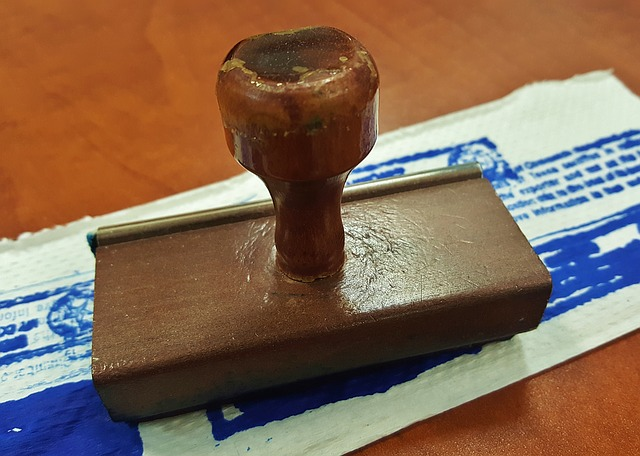
\includegraphics[width=0.5\textwidth]{../img/stamp}
\end{figure}
\begin{itemize}
\item En stämpel kan tillverkas -- motsvarar deklaration av klassen. 
 \item Det händer inget förrän man stämplar -- motsvarar \code{new}.
\item Då skapas avbildningar -- motsvarar instanser av klassen.


\end{itemize}
\end{Slide}


\begin{Slide}{Klassdeklarationer och instansiering}\SlideFontSmall
\setlength{\leftmargini}{0pt}
\begin{itemize}
\item Syntax för deklaration av klass: \\ \vspace{0.5em}{\SlideFontSize{13}{16}\code|class Klassnamn(parametrar){ medlemmar }|}\vspace{0.5em}



\item Exempel \Emph{deklaration}:
\begin{Code}
class Klassnamn(val attribut1: Int, attribut2: String){  
  val attribut3: Double = 42.0              //publikt oföränderligt attribut
  private var attribut3: Boolean = false    //privat medlem syns inte utåt
  def metod(parameter: Int) = parameter + 1 //funktion i klass kallas metod
  lazy val attr4 = Vector.fill(100000)(42.0)     //fördröjd initialisering 
}
\end{Code}

\item Parametrar initialiseras med de argument som ges vid \code{new}. 
\item Exempel \Emph{instansiering}:
\begin{Code}
val instansReferens = new Klassnamn(42, "hej")
\end{Code}

\item Attribut blir \Emph{publika} (alltså synliga utåt) om inte modifieraren \code{private} anges.
\item Parametrar som inte föregås av modifierare (t.ex. private val, val, var) blir attribut som är: \code{ private[this] val } och bara synliga i \Alert{denna} instans.

\end{itemize}
\end{Slide}


\begin{Slide}{Exempel: Klassen Complex i Scala}\SlideFontSmall
\begin{Code}
class Complex(val re: Double, val im: Double){
  def r  = math.hypot(re, im)
  def fi = math.atan2(re, im)
  def +(other: Complex) = new Complex(re + other.re, im + other.im)
  var imSymbol = 'i'
  override def toString = s"$re + $im$imSymbol"
}
\end{Code}

\begin{REPL}
scala> val c1 = new Complex(3, 4)
c1: Complex = 3.0 + 4.0i

scala> val polarForm = (c1.r, c1.fi)
polarForm: (Double, Double) = (5.0,0.6435011087932844)

scala> val c2 = new Complex(1, 2)
c2: Complex = 1.0 + 2.0i

scala> c1 + c2
res0: Complex = 4.0 + 6.0i
\end{REPL}

%TODO:
%  \begin{itemize} 
%  \item Bygg upp \code{case class Complex(re: Double, im: Double)} steg för steg inspirerat av Pins3ed kap 6 i likhet med hur de gör med Rational
%  \item Illustrera följande begrepp: this (behövs i max(that)), method overloading behövs för att plussa med både Complex och Double
%  \item Till fördjupningsövning: dekorera Double med metoderna im och re samt (Double, Double) med metoden ir (för irrational) med implicit klass
%  \item Till extrauppgift: implementera klassen Polar(r, fi) med polära koordinater \url{https://sv.wikipedia.org/wiki/Pol%C3%A4ra_koordinater}
%  \end{itemize}
\end{Slide}

\begin{Slide}{Exempel: Principen om enhetlig access}\SlideFontSmall
\begin{Code}
class Complex(val re: Double, val im: Double){
  val r  = math.hypot(re, im)
  val fi = math.atan2(re, im)
  def +(other: Complex) = new Complex(re + other.re, im + other.im)
  var imSymbol = 'i'
  override def toString = s"$re + $im$imSymbol"
}
\end{Code}
\pause
\begin{itemize}
\item Efter som attributen \code{re} och \code{im} är oföränderliga, kan vi lika gärna ändra i klass-implementationen och göra om metoderna \code{r} och \code{fi} till \code{val}-variabler utan att klientkoden påverkas. 

\item Då anropas \code{math.hypot} och \code{math.atan2} bara en gång vid initialisering (och inte varje gång som med \code{def}).

\item Vi skulle även kunna använda \code{lazy val} och då bara räkna ut \code{r} och \code{fi} om och när de verkligen refereras av klientkoden, annars inte.

\item Eftersom klientkoden inte ser skillnad på metoder och variabler, kallas detta \Emph{principen om enhetlig access}. (Många andra språk har \Alert{inte} denna möjlighet, tex Java.)

\end{itemize}

\end{Slide}


\begin{Slide}{Exempel: Motsvarande klass JComplex i Java}\SlideFontSmall
\javainputlisting[basicstyle=\SlideFontSize{5}{6}\ttfamily\selectfont]{../compendium/examples/JComplex.java}
\end{Slide}

\begin{Slide}{Exempel: Använda JComplex från Scala}
\begin{REPL}
$ javac JComplex.java 
$ scala
Welcome to Scala 2.11.8 (Java HotSpot(TM) 64-Bit Server VM, Java 1.8.0_66).
Type in expressions for evaluation. Or try :help.

scala> val jc1 = new JComplex(3, 4)
jc1: JComplex = 3.0 + 4.0i

scala> val polarForm = (jc1.getR, jc1.getFi)
polarForm: (Double, Double) = (5.0,0.6435011087932844)

scala> val jc2 = new JComplex(1, 2)
jc2: JComplex = 1.0 + 2.0i

scala> jc1 add jc2
res0: JComplex = 4.0 + 6.0i
\end{REPL}
\end{Slide}


\begin{Slide}{Exempel: Test av JComplex i Java}
\javainputlisting[basicstyle=\SlideFontSize{9}{11}\ttfamily\selectfont]{../compendium/examples/JComplexTest.java}
\begin{itemize}
\item Tupler finns inte i Java, så det går inte på ett enkelt sätt att i Java skapa par av värden somi Scala.

\item Operatornotation för metoder finns inte i Java, så man måste i Java använda punktnotation och skriva: \code{jc1.add(jc2)}
\end{itemize}
\end{Slide}


\Subsection{Instansiering: \texttt{new}}

\begin{Slide}{Instansiering med \texttt{new}}
Rita molbild med instanser av klassen Complex
\end{Slide}

\begin{Slide}{Instansiering med fabriksmetod}
\end{Slide}

\begin{Slide}{Instansiering med default-argument}
\end{Slide}

\begin{Slide}{Instansiering med alternativa fabriksmetoder}
\end{Slide}

\begin{Slide}{Förändringsbar eller oföränderlig?}
\end{Slide}


\Subsection{Referens saknas: \texttt{null}}

\begin{Slide}{Referens saknas: \texttt{null}}
\end{Slide}


\begin{Slide}{Konstruktor}
\end{Slide}

\begin{Slide}{Skräpsamling}
Destruktor
\end{Slide}

\Subsection{Synlighet}

\begin{Slide}{Synlighet}
definiera/förklara:
private
private[this]
\end{Slide}

\begin{Slide}{Kompanjonsobjekt}
\end{Slide}


\begin{Slide}{Synlighet av klassparametrar i klasser \& case-klasser}\SlideFontSmall
\code{private[this]} är \Alert{ännu} mer privat än \code{private} 
\begin{Code}
class Hemlis(private val hemlis: Int) {
  def ärSammaSom(annan: Hemlis) = hemlis == annan.hemlis   // Funkar!
}

class Hemligare(private[this] val hemlis: Int) {
  def ärSammaSom(annan: Hemligare) = hemlis == annan.hemlis //KOMPILERINGSFEL
}
\end{Code}
Vad händer om man inte skriver något? Olika för klass och case-klass:
\begin{Code}
class Hemligare(hemlis: Int) { // motsvarar private[this] val
  def ärSammaSom(annan: Hemligare) = hemlis == annan.hemlis //KOMPILERINGSFEL
}

case class InteHemlig(seMenInteRöra: Int) { // blir automatiskt val 
  def ärSammaSom(annan: InteHemlig): Boolean = 
    seMenInteRöra == annan.seMenInteRöra 
}

\end{Code}
\end{Slide}


\Subsection{Klasser i Java}

\begin{Slide}{Klasser i Java}
\end{Slide}

\begin{Slide}{Statiska medlemmar}
\end{Slide}


\Subsection{Getters och setters}

\begin{Slide}{Getters och setters i Java}
\end{Slide}

\begin{Slide}{Getters och setters i Scala}
\end{Slide}

\begin{Slide}{Ändra attributrepresentation utan att påverka existerande kod}
Complex som polära koordinater i Java med privat attribut
Complex som polära koordinater med publika attribut om man har enhetlig access
\end{Slide}


\Subsection{Implementation saknas: ???}

\begin{Slide}{Implementation saknas: ???}
\end{Slide}


\fi


%!TEX encoding = UTF-8 Unicode
%!TEX root = ../lect-week06.tex

%%%

\ifkompendium\else

\Subsection{Likhet}
\begin{Slide}{Referenslikhet eller strukturlikhet?}\SlideFontSmall
Det finns två \Alert{principiellt olika} sorters \Emph{likhet}:
\begin{itemize}
\item \Emph{Referenslikhet} \Eng{refernce equality} där två referenser anses lika om de refererar till \Emph{samma instans} i minnet.
\item \Emph{Strukturlikhet} \Eng{structural equality} där två referenser anses lika om de refererar till instanser med \Emph{samma innehåll}.

\pause

\item I Scala finns flera metoder som testar likhet:
\begin{itemize}\SlideFontSmall
\item metoden \code{eq} testar referenslikhet och \code{r1.eq(r2)} ger \code{true} om \code{r1} och \code{r2} refererar till \Emph{samma} instans.

\item metoden \code{ne} testar referens\textbf{o}likhet och \code{r1.ne(r2)} ger \code{true} om \code{r1} och \code{r2} refererar till \Alert{olika} instanser.

\item metoden \code{==} som anropar metoden \code{equals} som default testar referenslikhet men som \Alert{kan överskuggas} om man \Emph{själv vill bestämma} om det ska vara referenslikhet eller strukturlikhet.
\end{itemize}

\pause

\item Scalas \Emph{standardbibliotek} och \Emph{grundtyperna} \code{Int}, \code{String} etc. testar \Emph{strukturlikhet} genom metoden \code{==}
\pause
\item I Java är det annorlunda: symbolen \code{==} är ingen metod i Java utan specialsyntax som  testar referenslikhet mellan instanser, medan metoden \code{equals} kan överskuggas med valfri likhetstest.
\end{itemize}
\end{Slide}


\begin{Slide}{Exempel: referenslikhet och strukturlikhet}
I Scalas standardbibliotek har man överskuggat \code{equals} så att metoden \code{==} ger test av \Emph{strukturlikhet} mellan instanser:
\begin{REPL}
scala> val v1 = Vector(1,2,3)
v1: scala.collection.immutable.Vector[Int] = Vector(1, 2, 3)

scala> val v2 = Vector(1,2,3)
v2: scala.collection.immutable.Vector[Int] = Vector(1, 2, 3)

scala> v1 eq v2                //referenslikhetstest: olika instanser
res0: Boolean = false

scala> v1 ne v2
res1: Boolean = true

scala> v1 == v2                //strukturlikhetstest: samma innehåll
res2: Boolean = true

scala> v1 != v2
res3: Boolean = false
\end{REPL}
\end{Slide}


\begin{Slide}{Referenslikhet och egna klasser}
Om du inte gör något speciellt med dina egna klasser så ger metoden \code{==} test av \Emph{referenslikhet} mellan instanser:
\begin{REPLnonum}
scala> class Gurka(val vikt: Int)

scala> val g1 = new Gurka(42)
g1: Gurka = Gurka@2cc61b3b

scala> val g2 = new Gurka(42)
g2: Gurka = Gurka@163df259

scala> g1 == g2       // samma innehåll men olika instanser
res0: Boolean = false

scala> g1. vikt == g2. vikt
res1: Boolean = true
\end{REPLnonum}
\end{Slide}

\fi


%!TEX encoding = UTF-8 Unicode
%!TEX root = ../lect-week06.tex

%%%
\ifkompendium\else


\Subsection{Case-klasser och likhet}



\begin{Slide}{Varför case-klass?}
Med case-klasser får du mycket ''godis på köpet'':
\begin{itemize}
\item Skapa \Emph{oföränderlig datastruktur} med få kodrader.
\item Klassparametrar blir automatiskt publika \code{val}-attribut (inte \texttt{private[this]} som i vanliga klasser).
\item Du får en automatisk \Emph{toString} som ger klassens namn och värdet av alla \code{val}-attribut som ges av klassparametrarna.
\item Du slipper skriva \code{new} eftersom du får ett automatiskt kompanjonsobjekt med en fabriksmetod \code{apply} för indirekt instansiering där alla klassparametrarnas \code{val}-attribut initialiseras.
\item Metoden \code{==} ger \Emph{strukturlikhet} (och inte referenslikhet).
\end{itemize}
\end{Slide}



\begin{Slide}{Likhet och case-klasser}
Metoden \code{equals} är i case-klasser automatiskt överskuggad så att metoden \code{==} ger test av strukturlikhet. 
\begin{REPL}
scala> case class Gurka(vikt: Int)

scala> val g1 = Gurka(42)
g1: Gurka = Gurka(42)

scala> val g2 = Gurka(42)
g2: Gurka = Gurka(42)

scala> g1 eq g2          // olika instanser
res0: Boolean = false

scala> g1 == g2          // samma innehåll!
res1: Boolean = true
\end{REPL}
\end{Slide}



\begin{Slide}{Sammanfattning case-klass-godis}
Minneschecklista med ''godis'' i \code{case}-klasser så här långt:
\begin{enumerate}
\item klassparametrar blir \code{val}-attribut 
\item najs toString
\item slipper skriva \code{new}
\item == ger strukturlikhet
\pause~\\...
\end{enumerate}

\vspace{3em}Men vi har inte sett allt godis än... \\Vecka 8: Mönstermatchning.
\end{Slide}



\fi
%!TEX encoding = UTF-8 Unicode
%!TEX root = ../lect-week06.tex

%%%


\Subsection{Implementation saknas: ???}

\begin{Slide}{Implementation saknas: ???}
\begin{itemize}
\item Ofta vill man bygga kod iterativt och steg för steg lägga till olika funktionalitet.

\item Standardfunktionen \code{???} ger vid anrop undantaget \Alert{\texttt{NotImplementedError}} och kan användas på platser i koden där man ännu inte är färdig. 

\item \code{???} tillåter \Emph{kompilering av ofärdig kod}.

\pause

\item Undantag har bottentypen \code{Nothing} som är subtyp till \emph{alla} typer och kan därmed tilldelas referenser av godtycklig typ.

\begin{REPLnonum}
scala> lazy val sprängsSnart: Int = ???

scala> sprängsSnart + 42
scala.NotImplementedError: an implementation is missing
  at scala.Predef$.$qmark$qmark$qmark(Predef.scala:230)
  at .sprängsSnart$lzycompute(<console>:11)
  at .sprängsSnart(<console>:11)
\end{REPLnonum} 

\end{itemize}
\end{Slide}

\begin{Slide}{Exempel: ofärdig kod}
\begin{Code}[basicstyle=\SlideFontSize{9}{11}\ttfamily\selectfont]
case class Person(name: String, age: Int){
  def ärGammal: Boolean = ???   //def ännu ej bestämd
  def ärUng = !ärGammal
  def ärTonåring = age >= 13 && age <= 19
}
\end{Code}
\begin{REPLnonum}
scala> Person("Björn", 49).ärTonåring
res23: Boolean = false

scala> Person("Sandra", 35).ärUng
scala.NotImplementedError: an implementation is missing
  at scala.Predef$.$qmark$qmark$qmark(Predef.scala:230)
  at Person.ärGammal(<console>:12)
  at Person.ärUng(<console>:13)
\end{REPLnonum}
\end{Slide}


\Subsection{Klass-specifikationer}




\begin{Slide}{Specifikationer av klasser i Scala}\footnotesize
\begin{itemize}
\item Specifikationer av klasser innehåller information som \emph{den som ska implementera} klassen behöver veta.
\item Specifikationer innehåller liknande information som dokumentationen av klassen (scaladoc), som beskriver vad \emph{användaren} av klassen behöver veta.  
\end{itemize}
\begin{ScalaSpec}{Person}
/** Encapsulate immutable data about a Person: name and age. */ 
case class Person(name: String, age: Int = 0){
  /** Tests whether this Person is more than 17 years old. */
  def isAdult: Boolean = ???
}
\end{ScalaSpec}
\begin{itemize}
\item Specifikationer av Scala-klasser utgör i denna kurs ofullständig kod som kan kompileras utan fel. 
\item Saknade implementationer markeras med \code{???}
\item \Emph{Dokumentationskommentarer} utgör \Alert{krav} på implementationen.
\end{itemize}

\end{Slide}


\begin{Slide}{Specifikationer av klasser och objekt}
\begin{ScalaSpec}{MutablePerson}
/** Encapsulates mutable data about a person. */
class MutablePerson(initName: String, initAge: Int){
  /** The name of the person. */
  def getName: String = ???
  
  /** Update the name of the Person */
  def setName(name: String): Unit = ???

  /** The age of this person. */
  def getAge: Int = ???

  /** Update the age of this Person */
  def setAge(age: Int): Unit = ???

  /** Tests whether this Person is more than 17 years old. */
  def isAdult: Boolean = ???

  /** A string representation of this Person, e.g.: Person(Robin, 25) */
  override def toString: String = ???
}
object MutablePerson {
  /** Creates a new MutablePerson with default age. */
  def apply(name: String): MutablePerson = ???
}
\end{ScalaSpec}

\end{Slide}

\ifkompendium
Man brukar inte använda \code{get} och \code{set} i metodnamn i Scala. Mer senare om principen om enhetlig access \Eng{uniform access principle} och hur man gör ''setters'' som möjliggör tilldelningssyntax.
\fi


\begin{Slide}{Specifikationer av Java-klasser}
\begin{itemize}\small
\item Specificerar signaturer för konstruktorer och metoder. 
\item Kommentarerna utgör krav på implementationen.  
\item Används flitigt på extentor i EDA016, EDA011, EDA017...
\item Javaklass-specifikationerna \Alert{saknar} \Emph{implementationer} och behöver kompletteras med metodkroppar och klassrubriker innan de kan kompileras.
\end{itemize}
\begin{JavaSpec}{class Person}
/** Skapar en person med namnet name och åldern age. */
Person(String name, int age);

/** Ger en sträng med denna persons namn. */
String getName();

/** Ändrar denna persons ålder. */
void setAge(int age);

/** Anger åldersgränsen för när man blir myndig. */
static int adultLimit = 18;
\end{JavaSpec}
\end{Slide}


%!TEX encoding = UTF-8 Unicode
%!TEX root = ../lect-week06.tex

%%%

\ifkompendium\else

\Subsection{Grumligt-lådan}
\begin{Slide}{Grumligt-lådan}
Veckans skörd av lappar i ''grumligtlådan'':
\begin{multicols}{2}
\begin{lstlisting}[basicstyle=\SlideFontSize{7}{9},language=]
12	case class
8	Map och map
8	private, public
5	override
3	toString
3	kompanjonsobjekt
2	typparametrar [Int]
2	Specialfall, sekvensalgoritmer
\end{lstlisting}

\columnbreak

\begin{lstlisting}[basicstyle=\SlideFontSize{5}{6},language=]
1	lab pirates
1	Hur ska jag träna datastrukturer?
1	underscore i olika sammanhang
1	Stränginterpolator s"\$x" 
1	heap
1	Assume
1	Mutable / immutable
1	Vad är en typ och hur kan klass bli en typ?
1	tomma parenteser ()
1	skillnad mellan argument och parameter
1	pseudokod
1	Hur hitta buggar?
1	w04 datastrukturer
1	skillnad på olika parenteser \{[(
1	terminologi allmänt
1	uppdatering av variabler som refererar till varandra
1	val, lazy val, var
1	när använda terminal, editor, IDE?
1	Formattering/upplägg av kod, indrag, var ska objekt vara?
-	Bättre instruktioner på labbarna
-	bra med sammanfattning på slutet av föreläsningarna
\end{lstlisting}
\end{multicols}
\end{Slide}

\fi


%!TEX encoding = UTF-8 Unicode
%!TEX root = ../lect-week06.tex

%%%

\ifkompendium\else

\Subsection{Veckans uppgifter}
\begin{Slide}{Övning: \texttt{classes}}
\begin{itemize}\SlideFontSmall
%!TEX encoding = UTF-8 Unicode

%!TEX root = ../compendium2.tex

\item Kunna deklarera klasser med klassparametrar.
\item Kunna skapa objekt med \code{new} och konstruktorargument.
\item Förstå innebörden av referensvariabler och värdet \code{null}.
\item Förstå innebörden av begreppen instans och referenslikhet.
\item Kunna använda nyckelordet \code{private} för att styra synlighet i primärkonstruktor.
\item Förstå i vilka sammanhang man kan ha nytta av en privat konstruktor.
\item Kunna implementera en klass utifrån en specikation.
\item Förstå skillnaden mellan referenslikhet och strukturlikhet.
\item Känna till hur case-klasser hanterar likhet.
\item Förstå nyttan med att möjliggöra framtida förändring av attributrepresentation.
\item Känna till begreppen getters och setters.
\item Känna till accessregler för kompanjonsobjekt.
\item Känna till skillnaden mellan \code{==} och \code{eq}, samt \code{!=} versus \code{ne}.

\end{itemize}
\end{Slide}

\begin{Slide}{Laboration: \texttt{turtlegraphics}}
\begin{itemize}
%!TEX encoding = UTF-8 Unicode

%!TEX root = ../compendium.tex

\item Kunna skapa egna klasser.
\item Förstå skillnaden mellan klasser och objekt.
\item Förstå skillnaden mellan muterbara och omuterbara objekt.
\item Förstå hur ett objekt kan innehålla referenser till objekt av andra klasser, och varför detta kan vara användbart.
\item Träna på att fatta beslut om vilka datatyper som bäst passar en viss tillämpning.

\end{itemize}
\end{Slide}

\fi



\Lecture{7}{Arv}
%!TEX encoding = UTF-8 Unicode
%!TEX root = ../lect-week07.tex

%%%


%\begin{Slide}{TODO: Begrepp att förklara}
%  Tänk igenom ordningen:
%  \begin{itemize}
%    \item OO, arv, supertyp, subtyp, bastyp, polymorfism, ... 
%  \end{itemize}
%\end{Slide}

\ifkompendium\else

\Subsection{Vad är arv?}

\begin{Slide}{Vad är arv?}

\begin{minipage}{0.4\textwidth}
\raggedright Med arv kan man beskriva relationen \\
$X$ \Emph{är en} $Y$

\end{minipage}
\begin{minipage}{0.4\textwidth}
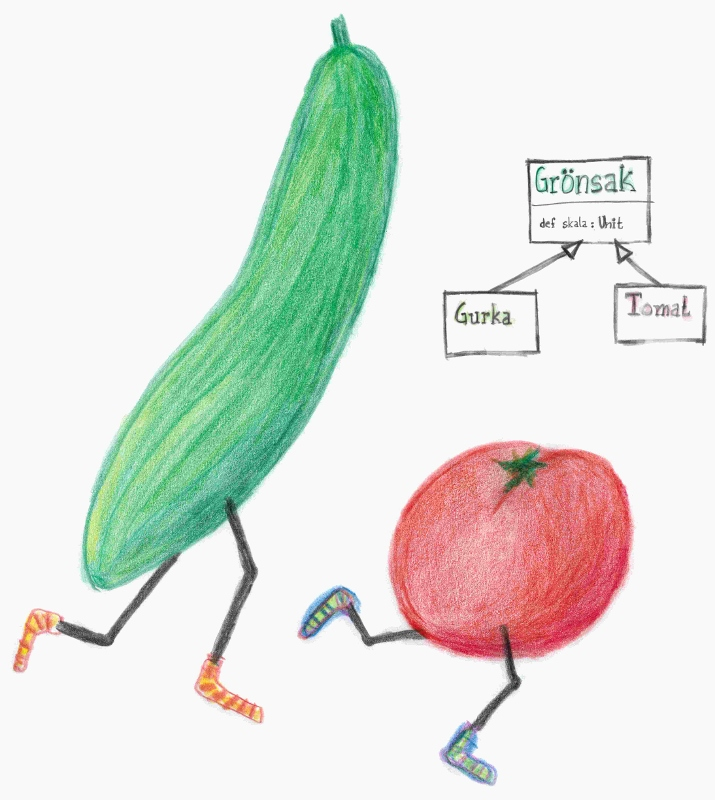
\includegraphics[width=1.5\textwidth]{../img/gurka-tomat-715x800}
\end{minipage} 
\end{Slide}


\begin{Slide}{Varför behövs arv?}
\begin{itemize}
\item Man kan använda arv för att dela upp kod i: 
\begin{itemize}
\item \Emph{generella} (gemensamma) delar och 
\item \Emph{specifika} (specialanpassade) delar.
\end{itemize}

\item Man kan åstadkomma \Emph{kontrollerad flexibilitet}: 
\begin{itemize}
\item Klientkod kan \Emph{utvidga} \Eng{extend} ett givet API med egna specifika tillägg.
\end{itemize}

\item Man kan använda arv för att deklarera en gemensam \Emph{bastyp} så att generiska samlingar kan ges en mer specifik elementtyp. 
\begin{itemize}
\item Det räcker att man vet bastypen för att kunna anropa gemensamma metoder på alla element i samlingen.
\end{itemize}
\end{itemize}
\end{Slide}


\begin{Slide}{Behovet av gemensam bastyp}\SlideFontSmall
\begin{REPL}
scala> class Gurka(val vikt: Int)

scala> class Tomat(val vikt: Int)

scala> val gurkor = Vector(new Gurka(200), new Gurka(300))
gurkor: scala.collection.immutable.Vector[Gurka] = 
  Vector(Gurka@60856961, Gurka@2fd953a6)
  
scala> gurkor.map(_.vikt)
res0: scala.collection.immutable.Vector[Int] = Vector(200, 300)

scala> val grönsaker = Vector(new Gurka(200), new Tomat(42))
grönsaker: scala.collection.immutable.Vector[Object] = 
  Vector(Gurka@669253b7, Tomat@5305c37d)

scala> grönsaker.map(_.vikt)
<console>:15: error: value vikt is not a member of Object
       grönsaker.map(_.vikt)
\end{REPL}
Hur ordna en mer specifik typ än \code{Vector[Object]}? \pause$\rightarrow$ Skapa en \Emph{bastyp}!
\end{Slide}




\begin{Slide}{Skapa en gemensam bastyp}
Typen \textit{\textbf{\texttt{Grönsak}}} är en \Emph{bastyp} i nedan arvshierarki:

\vspace{1em}
\begin{center}
\newcommand{\TextBox}[1]{\raisebox{0pt}[1em][0.5em]{#1}}
\tikzstyle{umlclass}=[rectangle, draw=black,  thick, anchor=north, text width=2cm, rectangle split, rectangle split parts = 3]
\begin{tikzpicture}[inner sep=0.5em]
\node [umlclass, rectangle split parts = 1, xshift=0cm] (BaseType)  {
            \textit{\textbf{\centerline{\TextBox{\code{Grönsak}}}}}
            %\nodepart[]{second}\TextBox{\code{val vikt: Int}}
        };
        
\node [umlclass, rectangle split parts = 1]  at (2cm,-2cm) (SubType1) {
            \textbf{\centerline{\TextBox{\code{Gurka}}}}
            %\nodepart[]{second} \TextBox{~}
        };  
                
\node [umlclass, rectangle split parts = 1] at (-2cm,-2cm) (SubType2)  {
            \textbf{\centerline{\TextBox{\code{Tomat}}}}
            %\nodepart[]{second} \TextBox{talk(): void}
        };        
\draw[umlarrow] (SubType1.north) -- ++(0,0.5) -| (BaseType.south);    
\draw[umlarrow] (SubType2.north) -- ++(0,0.5) -| (BaseType.south);            
\end{tikzpicture}

\pause
\vspace{2em} Pilen ~ \tikz\draw[umlarrow] (0,0) -- (0,0.5); ~ betecknar \Emph{arv} och utläses ''\Alert{är en}''

\pause
{\vspace{1em}\SlideFontSmall Typerna \code{Tomat} och \code{Gurka} är \Emph{subtyper} till den \Emph{abstrakta} typen \code{Grönsak}.}
\end{center}
\end{Slide}







\begin{Slide}{Skapa en gemensam bastyp med \texttt{trait} och \texttt{extends}}\SlideFontSmall
Med \code{trait Grönsak} kan klasserna \code{Gurka} och \code{Tomat} få en gemensam \Emph{bastyp} genom att båda \Emph{subtyperna} gör \code{extends Grönsak}:
\begin{REPL}
scala> trait Grönsak

scala> class Gurka(val vikt: Int) extends Grönsak

scala> class Tomat(val vikt: Int) extends Grönsak

scala> val grönsaker = Vector(new Gurka(200), new Tomat(42))
grönsaker: scala.collection.immutable.Vector[Grönsak] = 
  Vector(Gurka@3dc4ed6f, Tomat@2823b7c5)


\end{REPL}
\pause
Men det är fortfarande inte som vi vill ha det:
\begin{REPLnonum}
scala> grönsaker.map(_.vikt)
<console>:15: error: value vikt is not a member of Grönsak
       grönsaker.map(_.vikt)
\end{REPLnonum}
\end{Slide}



\begin{Slide}{En gemensam bastyp med gemensamma delar}\SlideFontSmall
Placera gemensamma medlemmar i bastypen:

\vspace{1em}
\begin{center}
\newcommand{\TextBox}[1]{\raisebox{0pt}[1em][0.5em]{#1}}
\tikzstyle{umlclass}=[rectangle, draw=black,  thick, anchor=north, text width=3cm, rectangle split, rectangle split parts = 3]
\begin{tikzpicture}[inner sep=0.5em]
\node [umlclass, rectangle split parts = 2, xshift=0cm] (BaseType)  {
            \textit{\textbf{\centerline{\TextBox{\code{Grönsak}}}}}
            \nodepart[]{second}\TextBox{\code{val vikt: Int}}
        };
        
\node [umlclass, rectangle split parts = 1]  at (2cm,-3cm) (SubType1) {
            \textbf{\centerline{\TextBox{\code{Gurka}}}}
            %\nodepart[]{second} \TextBox{~}
        };  
                
\node [umlclass, rectangle split parts = 1] at (-2cm,-3cm) (SubType2)  {
            \textbf{\centerline{\TextBox{\code{Tomat}}}}
            %\nodepart[]{second} \TextBox{talk(): void}
        };        
\draw[umlarrow] (SubType1.north) -- ++(0,0.5) -| (BaseType.south);    
\draw[umlarrow] (SubType2.north) -- ++(0,0.5) -| (BaseType.south);            
\end{tikzpicture}
\end{center}
\vspace{2em} 
\begin{itemize}
\item Alla grönsaker har attributet \code{val vikt}. 
\item Det specifika värdet på vikten definieras \Alert{inte} i bastypen. 
\item Medlemen \code{vikt} kallas  \Emph{abstrakt} eftersom den \Alert{saknar implementation}.
\end{itemize}
\end{Slide}





\begin{Slide}{Placera gemensamma delar i bastypen}

Vi inkluderar det gemensamma attributet \code{val vikt} som en \Emph{abstrakt medlem} i bastypen:

\begin{Code}
trait Grönsak { val vikt: Int }

class Gurka(val vikt: Int) extends Grönsak

class Tomat(val vikt: Int) extends Grönsak
\end{Code}
Nu vet kompilatorn att alla grönsaker har en vikt: 
\begin{REPL}
scala> val grönsaker = Vector(new Gurka(200), new Tomat(42))
grönsaker: scala.collection.immutable.Vector[Grönsak] = 
  Vector(Gurka@3dc4ed6f, Tomat@2823b7c5)

scala> grönsaker.map(_.vikt)
res0: scala.collection.immutable.Vector[Int] = Vector(200, 42)
\end{REPL}

\end{Slide}





\begin{Slide}{Scalas typhierarki och typen \texttt{Object}}
Den översta delen av typhierarkin i Scala: 
\vspace{1em}
\begin{center}
\newcommand{\TextBox}[1]{\raisebox{0pt}[1em][0.5em]{#1}}
\tikzstyle{umlclass}=[rectangle, draw=black,  thick, anchor=north, text width=2.5cm, rectangle split, rectangle split parts = 3]
\begin{tikzpicture}[inner sep=0.5em]
\node [umlclass, rectangle split parts = 1, xshift=0cm] (BaseType)  {
            \textit{\textbf{\centerline{\TextBox{\code{Any}}}}}
            %\nodepart[]{second}\TextBox{\code{def toString: String}}
        };
        
\node [umlclass, rectangle split parts = 1]  at (2cm,-2cm) (SubType1) {
            \textit{\textbf{\centerline{\TextBox{\code{AnyRef}}}}}
            %\nodepart[]{second} \TextBox{~}
        };  
                
\node [umlclass, rectangle split parts = 1] at (-2cm,-2cm) (SubType2)  {
            \textit{\textbf{\centerline{\TextBox{\code{AnyVal}}}}}
            %\nodepart[]{second} \TextBox{talk(): void}
        };        
\draw[umlarrow] (SubType1.north) -- ++(0,0.5) -| (BaseType.south);    
\draw[umlarrow] (SubType2.north) -- ++(0,0.5) -| (BaseType.south);            
\end{tikzpicture}
\end{center}
\begin{itemize}\SlideFontSmall
\item De numeriska typerna \code{Int}, \code{Double}, etc är subtyper till \Emph{\code{AnyVal}} och kallas \Emph{värdetyper} och lagras på ett speciellt, effektivt sätt i minnet.  
\item Alla dina egna klasser är subtyper till \Emph{\texttt{AnyRef}} och kallas \Emph{referenstyper} och kräver (direkt eller indirekt) konstruktion med \code{new}.
\item \texttt{AnyRef} motsvaras av \Alert{\code{java.lang.Object}} i JVM.
\end{itemize}
\end{Slide}



\begin{Slide}{Implicita supertyper till dina egna klasser}
Alla dina egna typer ingår underförstått i Scalas typhierarki:

\vspace{1em}
\begin{center}
\newcommand{\TextBox}[1]{\raisebox{0pt}[1em][0.5em]{#1}}
\tikzstyle{umlclass}=[rectangle, draw=black,  thick, anchor=north, text width=2cm, rectangle split, rectangle split parts = 3]
\begin{tikzpicture}[inner sep=0.5em, scale=0.8, every node/.style={scale=0.8}]
\node [umlclass, rectangle split parts = 1, xshift=0cm] at (0,-0.3cm)(BaseType)  {
            \textit{\textbf{\centerline{\TextBox{\code{Any}}}}}
            %\nodepart[]{second}\TextBox{\code{def toString: String}}
        };
        
\node [umlclass, rectangle split parts = 1]  at (2cm,-2cm) (SubType1) {
            \textit{\textbf{\centerline{\TextBox{\code{AnyRef}}}}}
            %\nodepart[]{second} \TextBox{~}
        };  
                
\node [umlclass, rectangle split parts = 1] at (-2cm,-2cm) (SubType2)  {
            \textit{\textbf{\centerline{\TextBox{\code{AnyVal}}}}}
            %\nodepart[]{second} \TextBox{talk(): void}
        };        
        
        
\node [umlclass, rectangle split parts = 1] at (2cm,-3.5cm) (SubSubType)  {
            \textit{\textbf{\centerline{\TextBox{\code{Grönsak}}}}}
            %\nodepart[]{second} \TextBox{talk(): void}
        }; 
        
\node [umlclass, rectangle split parts = 1] at (3.5cm,-5.25cm) (SubSubSubType1)  {
            \textbf{\centerline{\TextBox{\code{Gurka}}}}
            %\nodepart[]{second} \TextBox{talk(): void}
        }; 
                
\node [umlclass, rectangle split parts = 1] at (0.5cm,-5.25cm) (SubSubSubType2)  {
            \textbf{\centerline{\TextBox{\code{Tomat}}}}
            %\nodepart[]{second} \TextBox{talk(): void}
        }; 

                
\draw[umlarrow] (SubType1.north) -- ++(0,0.3) -| (BaseType.south);    
\draw[umlarrow] (SubType2.north) -- ++(0,0.3) -| (BaseType.south);   
\draw[umlarrow] (SubSubType.north) -- (SubType1.south);    
\draw[umlarrow] (SubSubSubType1.north) -- ++(0,0.3) -| (SubSubType.south);    
\draw[umlarrow] (SubSubSubType2.north) -- ++(0,0.3) -| (SubSubType.south);                   
\end{tikzpicture}
\end{center}
\end{Slide}


\begin{Slide}{Vad är en trait?}
\begin{itemize}
\item \Alert{Trait} betyder \Emph{egenskap} på engelska.

\item En trait liknar en klass, \Alert{men} speciella regler gäller:  

\begin{itemize}

\item den \Emph{kan} innehålla delar som \Emph{saknar implementation}

\item den \Emph{kan mixas} med flera andra traits så att olika koddelar kan återanvändas på flexibla sätt. 

\item den \Alert{kan inte} instansieras direkt som den är; den måste återanvändas genom arv.

\item den \Alert{kan inte} ha klassparametrar eller konstruktorer
\end{itemize}

\pause
\item {\SlideFontSmall Jämförelse med Java:} 
\begin{itemize}\SlideFontTiny
\item En Scala-trait liknar det som i Java kallas \jcode{interface}, men man kan göra mer med Scala-traits: färre begränsningar, fler abstraktionsmöjligheter.

\item En Scala-trait med enbart abstrakta medlemmar kompileras till bytekod i JVM:en som kan användas från Java-kod precis som ett Java-interface.
\end{itemize}
\end{itemize}

\end{Slide}

\begin{Slide}{Vad används en trait till?}
En \code{trait} används för att skapa en bastyp som kan vara hemvist för gemensamma delar hos subtyper:
\begin{Code}
trait Bastyp { val x = 42 }                 // Bastyp har medlemmen x
class Subtyp1 extends Bastyp { val y = 43 } // Subtyp1 ärver x, har även y
class Subtyp2 extends Bastyp { val z = 44 } // Subtyp2 ärver x, har även z
\end{Code}
\pause\vspace{-0.5em}
\begin{REPL}
scala> val a = new Subtyp1
a: Subtyp1 = Subtyp1@51016012

scala> a.x
res0: Int = 42

scala> a.y
res1: Int = 43

scala> a.z
<console>:15: error: value z is not a member of Subtyp1

scala> new Bastyp
<console>:13: error: trait Bastyp is abstract; cannot be instantiated
\end{REPL}

\end{Slide}


\begin{Slide}{En trait kan ha abstrakta medlemmar}
\begin{Code}
trait X { val x: Int }   // x är abstrakt, d.v.s. saknar implementation
class A extends X { val x = 42 }   // x ges en implementation
class B extends X { val x = 43 }   // x ges en annan implementation
\end{Code}
\pause\vspace{-0.5em}
\begin{REPL}
scala> val a = new A
a: A = A@5faeada1

scala> val b = new B
b: B = B@cb51256

scala> val xs = Vector(a,b)
xs: scala.collection.immutable.Vector[X] = Vector(A@5faeada1, B@cb51256)

scala> xs.map(_.x)
res0: scala.collection.immutable.Vector[Int] = Vector(42, 43)

scala> class Y { val y: Int }
  error: class Y needs to be abstract, since value y is not defined
  
scala> trait Z(x: Int)
  error: traits or objects may not have parameters

\end{REPL}
\end{Slide}


\begin{Slide}{Terminologi och nyckelord}\SlideFontTiny

\begin{tabular}{r  l}
\Emph{subtyp}           & en typ som ärver en supertyp\\
\Emph{supertyp}         & en typ som ärvs av en subtyp\\
\Emph{bastyp}           & en typ som är rot i ett arvsträd\\
\Emph{abstrakt medlem}  & en medlem som saknar implementation\\
\Emph{konkret medlem}   & en medlem som ej saknar implementation\\
\Emph{abstrakt typ}     & en typ som kan ha abstrakta medlemmar; kan ej instansieras\\
\Emph{konkret typ}      & en typ som ej har abstrakta medlemmar; kan instansieras\\
\code|class|            & en klass är en konkret typ som \Alert{ej kan ha abstrakta medlemmar}\\
\code|abstract class|   & en klass är en abstrakt typ som \Emph{kan ha parametrar}\\
\code|trait|            & är en abstrakt typ som \Alert{ej kan ha parametrar} men \Emph{kan mixas in}\\
\code|extends|          & står före en supertyp, medför arv av supertypens medlemmar\\
\code|override|         & en medlem överskuggar (byter ut) en medlem i en superttyp\\
\code|protected|        & gör en medlem synlig i subtyper till denna typ (jmf \code|private|)\\
\code|final gurka|      & gör medlemen gurka final: förhindrar överskuggning\\
\code|final class|      & gör klassen final: förhindrar vidare subtypning\\
\code|sealed trait|     & förseglad trait: bara de direkta subtyperna i denna kodfil\\
\code|super.gurka|      & refererar till supertypens medlem \code|gurka| (jmf \code|this|)\\
\end{tabular}

\pause
\begin{tikzpicture}[overlay]
     \node at (10.7,0.6) {
\includegraphics[scale=0.36]{../img/ttsuper}};
\end{tikzpicture}


\end{Slide}


\begin{Slide}{Abstrakta och konkreta medlemmar}
\vspace{-0.5em}\scalainputlisting[numbers=left,numberstyle=,basicstyle=\fontsize{6}{7}\ttfamily\selectfont]{../compendium/examples/workspace/w07-inherit/src/vego1.scala}
\end{Slide}


\begin{Slide}{Undvika kodduplicering med hjälp av arv}
\scalainputlisting[numbers=left,numberstyle=,basicstyle=\fontsize{6}{7.3}\ttfamily\selectfont]{../compendium/examples/workspace/w07-inherit/src/vego2.scala}
\end{Slide}




\begin{Slide}{Varför kan kodduplicering orsaka problem?}
\begin{itemize}
\item Mer att skriva (inte jättestort problem)
\pause
\item Fler kodrader att läsa och förstå
\pause
\item Fler kodrader som påverkas vid tillägg
\pause

\item Fler kodrader att underhålla: 
\begin{itemize}
\item Om man rättar en bug på ett ställe måste man komma ihåg att göra \Alert{exakt samma ändring} på alla de ställen där kodduplicering förekommer $\rightarrow$ \Alert{risk för nya buggar}
\end{itemize}	

\pause

\item Principen på engelska: \code{ DRY == "Don't Repeat Yourself!"}

\pause

\item {Men det kan finnas tillfällen när kodduplicering faktiskt är att föredra: t.ex. om man vill att olika delar av koden ska vara helt oberoende av varandra.}
\end{itemize}	
\end{Slide}




\begin{Slide}{Överskuggning}
\vspace{-0.5em}\scalainputlisting[numbers=left,numberstyle=,basicstyle=\fontsize{6}{7.3}\ttfamily\selectfont]{../compendium/examples/workspace/w07-inherit/src/vego3.scala}
\end{Slide}

\begin{Slide}{En final medlem kan ej överskuggas}
\vspace{-0.5em}\scalainputlisting[numbers=left,numberstyle=,basicstyle=\fontsize{6}{7.3}\ttfamily\selectfont]{../compendium/examples/workspace/w07-inherit/src/vego4.scala}
\end{Slide}


\begin{Slide}{Protected ger synlighet begränsad till subtyper}
\begin{REPL}
scala> trait Super { 
         private val minHemlis = 42
         protected val vårHemlis = 42
       }

scala> class Sub extends Super { def avslöjad = minHemlis } 
error: not found: value minHemlis

scala> class Sub extends Super { def avslöjad = vårHemlis } 
       
scala> val s = new Sub
s: Sub = Sub@2eee9593

scala> s.avslöjad
res0: Int = 42

scala> s.minHemlis
error: value minHemlis is not a member of Sub       

scala> s.vårHemlis
error: Access to protected value vårHemlis not permitted 
\end{REPL}
\end{Slide}


\begin{Slide}{Filnamnsregler och -konventioner}
\begin{itemize}
\item Java
\begin{itemize}
\item I Java får man bara ha \Alert{en enda} publik klass per kodfil.
\item I Java måste kodfilen ha \Alert{samma namn} som den publika klassen, t.ex. \code{KlassensNamn.java}
\end{itemize}
\item Scala
\begin{itemize}
\item I Scala får man ha \Emph{många} klasser/traits/singelobjekt i samma kodfil.
\item I Scala får man döpa kodfilerna \Emph{oberoende} av deras innehåll. \pause Dessa \Emph{konventioner} används:
\begin{itemize}
\item Om en kodfil bara innehåller \Emph{en enda} klass/trait/singelobjekt ge filen samma namn som innehållet, t.ex. \code{KlassensNamn.scala} 
\item Om en kodfil innehåller \Emph{flera} saker, döp filen till något som återspeglar hela innehållet och använd \Emph{liten begynnelsebokstav}, t.ex. \code{drawing.scala} eller \code{bastypensNamn.scala} 
\end{itemize}


\end{itemize}

\end{itemize}
\end{Slide}


\begin{Slide}{Klasser, arv och klassparametrar}\SlideFontTiny
Klasser kan ärva klasser. Om superklassen har klassparametrar måste primärkonstruktor ges argument efter \code{extends}.

\scalainputlisting[numbers=left,numberstyle=,basicstyle=\fontsize{6.4}{7.7}\ttfamily\selectfont]{../compendium/examples/workspace/w07-inherit/src/personExample1.scala}

\end{Slide}


\begin{Slide}{Inmixning}\SlideFontTiny
Man kan ärva flera traits. Detta kallas inmixning \Eng{mix-in} och görs med \code{with}.
\scalainputlisting[numbers=left,numberstyle=,basicstyle=\fontsize{6.4}{7.7}\ttfamily\selectfont]{../compendium/examples/workspace/w07-inherit/src/personExample2.scala}
\end{Slide}


\begin{Slide}{Statisk och dynamisk typ}\SlideFontSmall
\begin{Code}
    var p: Person = new Forskare("Robin Smith", "Lund", "Professor Dr")
\end{Code}
\begin{itemize}
\item Den \Emph{statiska typen} för \code{p} är \code{Person} vilket gör att vi sedan kan låta \code{p} referera till andra instanser som är av typen Person.
\begin{Code}
p = new Student("Kim Robinson", "Lund", "Data")
\end{Code}

\pause

\item Med ''statisk typ'' menas den typinformation som kompilatorn känner till vid kompileringstid.

\pause
\item Den \Emph{dynamiska typen}, även kallad \Emph{körtidstypen}, som gäller under körning är här mer specifik och mångfaceterad: \code{p} är efter tilldelning nu Student, Person och Akademiker (men inte Examinerad). 

\pause

\item Man kan undersöka om den dynamiska typen för \code{p} är \code{EnVissTyp} med  \code{p.isInstanceOf[EnVissTyp]}

\pause

\item Man kan säga åt kompilatorn: \emph{''jag garanterar att p är av typen \code{EnVissTyp} så du kan omforma den till \code{EnVissTyp}''} med  \code{p.asInstanceOf[EnVissTyp]} \\ \pause (detta är inte så vanligt i normal Scala-kod) 
\end{itemize}
\end{Slide}


\begin{Slide}{\texttt{isInstanceOf} och \texttt{asInstanceOf}}\SlideFontTiny
Testa körtidstyp med \code{isInstanceOf[Typ]}. Lova kompilatorn (och ta själv ansvar för) att det är en viss körtidstyp med \code{asInstanceOf[Typ]}.
\scalainputlisting[numbers=left,numberstyle=,basicstyle=\fontsize{6.2}{7.5}\ttfamily\selectfont]{../compendium/examples/workspace/w07-inherit/src/personExample3.scala}
\end{Slide}



\begin{Slide}{Polymorfism och dynamisk bindning}\SlideFontTiny
\begin{Code}[basicstyle=\SlideFontSize{6.2}{7.5}\ttfamily\selectfont]
trait Robot { def work(): Unit }

case class CleaningBot(name: String) extends Robot {
  override def work(): Unit = println(" Städa Städa")
}

case class TalkingBot(name: String) extends Robot {
  override def work(): Unit = println(" Prata Prata")
}
\end{Code}
\Emph{Polymorfism} betyder ''många former''. Referenserna r och bot nedan kan ha olika ''former'', d.v.s de kan referera till olika sorters robotar. \\ \Emph{Dynamisk bindning} innebär att körtidstypen avgör vilken metod som körs.
\begin{REPL}[basicstyle=\color{white}\SlideFontSize{6.2}{7.5}\ttfamily\selectfont]
scala> def robotDoWork(bot: Robot) = { print(bot); bot.work }

scala> var r: Robot = new CleaningBot("Wall-E")

scala> robotDoWork(r)
CleaningBot(Wall-E) Städa Städa

scala> r = new TalkingBot("C3PO")

scala> robotDoWork(r)
TalkingBot(C3PO) Prata Prata
\end{REPL}
\end{Slide}

\Subsection{Uppräknade värden}


\begin{Slide}{Uppräknade värden med heltal}\SlideFontSmall
Vi kan använda heltalskonstanter för att representera olika färger.
\begin{Code}
object Färg {
  val Spader = 1
  val Hjärter = 2
  val Ruter = 3
  val Klöver = 4
}
\end{Code}
\begin{Code}[language=,keywords={case,class}]
case class Kort(färg: Int, valör: Int)
\end{Code}

Vi kan nu använda våra uppräknade färgvärden så här:
\begin{REPL}
scala> import Färg._
scala> Kort(Ruter, 7)
\end{REPL}
\pause Men kompilatorn \Alert{kan inte hindra} denna bugg:
\begin{REPL}
scala> Kort(42, 7)
\end{REPL}

\end{Slide}


\begin{Slide}{Uppräknade värden med case-objekt}\SlideFontSmall
Vi kan använda case-objekt för att representera olika färger.
\begin{Code}[language=,keywords={sealed,trait,object,case,class,extends}]
sealed trait Färg
case object Spader  extends Färg
case object Hjärter extends Färg
case object Ruter   extends Färg
case object Klöver  extends Färg

case class Kort(färg: Färg, valör: Int)
\end{Code}

Vi kan nu använda våra uppräknade färgvärden så här:
\begin{REPL}
scala> Kort(Ruter, 7)

scala> Kort(Spader, 1)
\end{REPL}
\begin{itemize}
\item Kompilatorn \Emph{garanterar} att vi bara använder exakt dessa färger.

\item Nyckelordet \code{sealed} förhindrar fler subtyper förutom de som finns här.

\item \code{case} före \code{object} ger en najs \code{toString} och möjliggör matchning \\
(mer om matchning i w08).

\end{itemize}

\end{Slide}

\begin{Slide}{Uppräknade värden i samling}\SlideFontSmall
Vi kan placera case-objekten i en samling som kan användas i loopar. \\ Ett lämpligt ställe för en sådan samling är i kompanjonsobjektet till Färg.
\begin{Code}
sealed trait Färg
object Färg { 
  val values = Vector(Spader, Hjärter, Ruter, Klöver)
}
case object Spader extends Färg
case object Hjärter extends Färg
case object Ruter extends Färg
case object Klöver extends Färg
\end{Code}

\begin{REPL}
scala> val allaEss = for (f <- Färg.values) yield Kort(f, 1)
\end{REPL}
\end{Slide}


\begin{Slide}{Uppräknade värden med heltalsomvandling}\SlideFontSmall
Med en \code{sealed abstract class} och ett heltalsattrribut \code{toInt} som klassparameter kan vi erbjuda omvandling till heltal.
\begin{Code}
sealed abstract class Färg(final val toInt: Int)
object Färg { 
  val values = Vector(Spader, Hjärter, Ruter, Klöver)
}
case object Spader  extends Färg(0)
case object Hjärter extends Färg(1)
case object Ruter   extends Färg(2)
case object Klöver  extends Färg(3)
\end{Code}

\begin{REPL}
scala> Kort(Ruter, 1).färg.toInt
res0: Int = 2
\end{REPL}
Nyckelordet \code{abstract} förhindrar instansiering av \code{Färg}. \\
Nyckelordet \code{final} förhindrar överskuggning av attributet \code{toInt}. \\
Nyckelordet \code{sealed} förhindrar vidare subtypning av \code{Färg}.
\end{Slide}



\Subsection{Exempel: Shape}


\begin{Slide}{Exempel: shapes1.scala}
Typisk scala-kod: En trait som bastyp åt flera case-klasser.
\scalainputlisting[numbers=left,numberstyle=,basicstyle=\fontsize{6.4}{7.7}\ttfamily\selectfont]{../compendium/examples/workspace/w07-inherit/src/shapes1.scala}
\end{Slide}

\begin{Slide}{Exempel: shapesTest1.scala}
Test av konkreta subklasser till bastypen \code{Shape}.
\scalainputlisting[numbers=left,numberstyle=,basicstyle=\fontsize{6.4}{7.7}\ttfamily\selectfont]{../compendium/examples/workspace/w07-inherit/src/shapesTest1.scala}

\begin{REPL}
Rectangle((100.0,100.0),(75.0,120.0))
Rectangle((141.0,183.0),(75.0,120.0))
Triangle((0.0,0.0),(4.0,0.0),(4.0,3.0))
Triangle((1.0,1.0),(4.0,0.0),(4.0,3.0))
Triangle((0.0,0.0),(4.0,0.0),(4.0,3.0))
\end{REPL}
\end{Slide}


\begin{Slide}{Exempel: draw.scala}
Två traits som kan användas för att ''koppla ihop'' kod och minimera ändringar av befintlig kod:
\scalainputlisting[numbers=left,numberstyle=,basicstyle=\fontsize{7}{9}\ttfamily\selectfont]{../compendium/examples/workspace/w07-inherit/src/draw.scala}

\pause
\setlength{\leftmargini}{0pt}
\begin{itemize}\SlideFontSmall
\item  Traits som använda för att abstrahera implementation och möjliggöra uppfyllandet av ett slags ''kontrakt'' om vad som ska finnas kallas \Emph{gränssnitt} \Eng{interface} och är grunden för skapandet av ett flexibelt api. 

\item Implementationen av de delar vi vill kunna ändra senare placeras i subtyper som inte används direkt av klientkoden. 

\item Vi visar bara information om vad som erbjuds men inte hur det ser ut ''inuti''.

\end{itemize}
\end{Slide}

\begin{Slide}{Exempel: shapes2.scala}\SlideFontTiny
Genom att \Emph{mixa in} vår \code{trait CanDraw} kan en rektangel nu även ritas ut:

\scalainputlisting[numbers=left,numberstyle=,basicstyle=\fontsize{6.5}{7.8}\ttfamily\selectfont]{../compendium/examples/workspace/w07-inherit/src/shapes2.scala}

\pause
\vspace{-0.5em}Notera: ingen ändring i \code {Shape}! Vi behöver nu bara ett \Emph{\code{DrawingWindow}}...
\end{Slide}


\begin{Slide}{Exempel: SimpleDrawingWindow.scala}\SlideFontTiny
\vspace{-0.35em}
Vi skapar en ny klass som ärver \code{SimpleWindow}, som \Alert{dessutom} även \Emph{är ett} \code{DrawingWindow}, tack vare \Emph{inmixning} med nyckelordet \code{with}.\\
Observera att vi måste skicka vidare klassparametrarna till superklassens konstruktor. 

\scalainputlisting[numbers=left,numberstyle=,basicstyle=\fontsize{6.4}{7.7}\ttfamily\selectfont]{../compendium/examples/workspace/w07-inherit/src/SimpleDrawingWindow.scala}

\pause
\vspace{-0.35em}
\scalainputlisting[numbers=left,numberstyle=,basicstyle=\fontsize{6.4}{7.7}\ttfamily\selectfont]{../compendium/examples/workspace/w07-inherit/src/shapesTest2.scala}
\end{Slide}


%\begin{Slide}{Exempel: Robot}
%\begin{center}
%\newcommand{\TextBox}[1]{\raisebox{0pt}[1em][0.5em]{#1}}
%\begin{tikzpicture}[inner sep=0.5em]
%\node [umlclass, rectangle split parts = 2, xshift=0cm] (AbstractRobot)  {
%            \textit{\textbf{\centerline{\TextBox{AbstractRobot}}}}
%            \nodepart[]{second}\TextBox{work(): void}
%        };
%        
%\node [umlclass, rectangle split parts = 2]  at (2cm,-3cm) (MuteRobot) {
%            \textbf{\centerline{\TextBox{MuteRobot}}}
%            \nodepart[]{second} \TextBox{~}
%        };  
%                
%\node [umlclass, rectangle split parts = 2] at (-2cm,-3cm) (TalkingRobot)  {
%            \textbf{\centerline{\TextBox{TalkingRobot}}}
%            \nodepart[]{second} \TextBox{talk(): void}
%        };        
%\draw[umlarrow] (TalkingRobot.north) -- ++(0,0.5) -| (AbstractRobot.south);    
%\draw[umlarrow] (MuteRobot.north) -- ++(0,0.5) -| (AbstractRobot.south);            
%\end{tikzpicture}
%\end{center}
%\end{Slide}






\begin{Slide}{Attribut och metoder i UML-diagram}
\begin{center}
\begin{tikzpicture}
\node (Class) [umlclass, rectangle split parts = 3, xshift = -2cm, yshift=-1.5cm, text width = 4.2cm, scale=0.8]  {
            \textbf{\centerline{Name}}
            \nodepart[]{second}attr1: Type \newline attr2: Type
            \nodepart[]{third}method1(a: Type): Type \newline  method2(b: Type): Type
       };
\node (explain1)[above of = Class, yshift=1cm, text width=4.9cm]{En klass i ett \Emph{UML}-diagram kan ha 3 delar:};
\node (explain2)[below of = Class, yshift=-1cm]{Ibland utelämnar man typerna.};



\node [umlclass, rectangle split parts = 3]  at (4,0) (Robot) {
            \textbf{\centerline{Robot}}
            \nodepart[]{second}name: String
            \nodepart[]{third}work(): Unit
       };
\node [umlclass, rectangle split parts = 3]  at (4, -3) (TalkingRobot)  {
            \textbf{\centerline{TalkingRobot}}
            \nodepart[]{second} phrase: String           
            \nodepart[]{third}speak(): Unit
        };        
\draw[umlarrow] (TalkingRobot.north) -- ++(0,0.8) -| (Robot.south);        
\end{tikzpicture}
\end{center}
\hskip2em\href{https://en.wikipedia.org/wiki/Class_diagram}{\SlideFontTiny en.wikipedia.org/wiki/Class\_diagram}
\end{Slide}




\fi
%!TEX encoding = UTF-8 Unicode
%!TEX root = ../lect-week07.tex

%%%


%\begin{Slide}{TODO: Begrepp att förklara}
%  Tänk igenom ordningen:
%  \begin{itemize}
%    \item OO, arv, supertyp, subtyp, bastyp, polymorfism, ... 
%  \end{itemize}
%\end{Slide}


\Subsection{Överskugging}

\begin{Slide}{Medlemmar, arv och överskuggning}\SlideFontTiny
\begin{multicols}{2}
Olika sorters överskuggningsbara medlemmar i klasser och traits i \Emph{Scala}:
\begin{itemize}
\item \code{def}
\item \code{val}
\item \code{lazy val}
\item \code{var}
\end{itemize}


\columnbreak

\pause

Olika sorters överskuggningsbara instansmedlemmar i \Emph{Java}:
\begin{itemize}
\item variabel 
\item metod
\end{itemize}

{\SlideFontTiny Medlemmar som är \jcode{static} kan ej överskuggas (men döljas) vid arv.}

\vspace{0.5em}
\end{multicols}

\pause
\begin{itemize}\SlideFontTiny
\item När man överskuggar \Eng{override} en medlemmen med en annan medlem med samma namn i en subtyp, får denna medlem en (ny) implementation. 

\item När man konstruerar ett objektorienterat språk gäller det att man definierar sunda överskuggningsregler vid arv. Detta är förvånansvärt knepigt.

\item Singelobjekt kan ej ärvas (och medlemmar i singelobjekt kan därmed ej överskuggas).
\end{itemize}
\end{Slide}


\begin{Slide}{Fördjupning: Regler för överskuggning i Scala} \SlideFontTiny
\label{slideW07:overriderules}
En medlem M1 i en supertyp får överskuggas av en medlem M2 i en subtyp, enligt dessa regler:
\begin{enumerate}
\item M1 och M2 ska ha samma namn och typerna ska matcha.
\item \code{def} får bytas ut mot: \code{def}, \code{val}, \code{var}, \code{lazy val}
\item \code{val} får bytas ut mot: \code{val}, och om M1 är abstrakt mot en \code{lazy val}.
\item \code{var} får bara bytas ut mot en \code{var}.
\item \code{lazy val} får bara bytas ut mot en \code{lazy val}.
\item Om en medlem i en supertyp är abstrakt \emph{behöver} man inte använda nyckelordet \code{override} i subtypen. (Men det är bra att göra det ändå så att kompilatorn hjälper dig att kolla att du verkligen överskuggar något.) 
\item Om en medlem i en supertyp är konkret \emph{måste} man använda nyckelordet \code{override} i subtypen, annars ges kompileringsfel.
\item M1 får inte vara \code{final}.
\item M1 får inte vara \code{private} eller \code{private[this]}, men kan vara \code{private[X]} om M2 också är \code{private[X]}, eller \code{private[Y]} om X innehåller Y.   
\item Om M1 är \code{protected} måste även M2 vara det.

\end{enumerate}
\end{Slide}

\ifkompendium\else
\begin{Slide}{Fördjupning: Regler för överskuggning i Java}
\url{http://docs.oracle.com/javase/tutorial/java/IandI/override.html}
\end{Slide}
\fi

\Subsection{Trait eller abstrakt klass?}

\begin{Slide}{Trait eller abstrakt klass?} 
\SlideFontSmall
\label{slideW07:traitorclass}
\begin{multicols}{2}
Använd en \Emph{trait} som supertyp om...
\begin{itemize}
\item ...du är osäker på vilket som är bäst. (Du kan alltid ändra till en abstrakt klass senare.)
\item ...du vill kunna mixa in din trait tillsammans med andra traits.
\item ...du bara har abstrakta medlemmar. 
\end{itemize}

\columnbreak

Använd en \Alert{abstract class} som supertyp om...
\begin{itemize}
\item ...du vill ge supertypen en parameter vid konstruktion.
\item ...du vill ärva supertypen från klasser skrivna i Java.
\item ...du vill minimera vad som behöver omkompileras vid ändringar. 
\end{itemize}


\end{multicols}
\end{Slide}


\Subsection{\texttt{super}}

\begin{Slide}{\texttt{super}}
\begin{REPL}
scala> class X { def gurka = "super pepinos" }

scala> class Y extends X { override def gurka = ":("; def sup = super.gurka }

scala> val y = new Y
y: Y = Y@26ba2a48

scala> y.gurka
res0: String = :(
\end{REPL}

\pause
\begin{REPLnonum}
scala> y.sup
res1: String = super pepinos

\end{REPLnonum}


\pause
\begin{tikzpicture}[overlay]
     \node at (7.5,1.5) {
\includegraphics[scale=0.5]{../img/ttsuper}};
\end{tikzpicture}

\end{Slide}


%\begin{Slide}{Designexempel: Klassen ???}\small
%TODO:
%  \begin{itemize} 
%  \item 
%  \end{itemize}
%\end{Slide}











%!TEX encoding = UTF-8 Unicode
%!TEX root = ../lect-week07.tex

%%%

\ifkompendium\else



\Subsection{Nästa vecka: kontrollskrivning}
\begin{Slide}{Obl. kontrollskrivning: 25/10 kl 14:00-19 Gasquesalen}\SlideFontSmall
Kontrollskrivningen motsvarar i omfång en \Alert{halv} ordinarie tentamen och är uppdelad i två delar; del A och del B. 
\begin{itemize}\SlideFontTiny

\item Del A omfattar $20\%$ av den maximala poängsumman och innehåller uppgifter med korta svar (likt övningarna): ''ange typ och värde''.
\item Del B omfattar $80\%$ av den maximala poängsumman och innehåller uppgifter med svar i form av kod.

\item Maximal poäng på kontrollskrivningen är 50p. (Ordinarie tenta 100p)

\item Om du erhåller \code{p} poäng på kontrollskrivningen bidrar du med \code{(p / 10.0).round} i individuell bonuspoäng inför sammanräkningen av samarbetsbonus. 


\item Din samarbetsbonus är medelvärdet av poängen från dig och de av dina gruppmedlemmar som skriver kontrollskrivningen enligt denna beräkning:
\begin{Code}
  def collaborationBonus(points: Seq[Int]): Int =
    (points.sum / points.size.toDouble).round.toInt
\end{Code}

\item Samarbetsbonus motsvarar max 5\% av totala ordinarie tentapoäng.


\item Samarbetsbonus påverkar inte om du blir godkänd på tentan, men kan påverka vilket betyg du får. 


\end{itemize}
\end{Slide}


\begin{Slide}{Obligatorisk kontrollskrivning: instruktioner}
\Emph{Medtag}: \\ legitimation, penna blyerts, penna i avvikande färg helst röd, \\ ev. förtäring och \Alert{Scala Quickref/Java Snabbref}.

\vspace{2em}\begin{itemize}
\item Moment 1, ca 2,5h: \Emph{Lösning av uppgifterna}. 
\begin{itemize} 
\item Du löser uppgifterna individuellt med blyertspenna. 
\item När du är klar lämnar du in alla dina svar. 
\end{itemize}
\item Moment  2: \Emph{Parvis kamraträttning}.
\item Moment 3: \Emph{Bedömning av rättning}.
\end{itemize}
\end{Slide}

\begin{Slide}{Obligatorisk kontrollskrivning: instruktioner}
\begin{itemize}
\item Moment 1, ca 2,5h: \Emph{Lösning av uppgifterna}. 
 
\item Moment  2: \Emph{Parvis kamraträttning}. 
\begin{itemize}

\item
Ni  sätter  er  parvis  och  får  ut  rättningsmallen  som  ni läser. 

\item Efter  ca  10  minuter  får  ni  ut  två andra  personers  skrivningar  som  ni  rättar enligt  anvisningarna  i  rättningsmallen.  

\item Medtag och använd penna med avvikande färg, helst röd.

\item När  rättningstiden  är  slut  samlar  vi in alla rättade skrivningarna.
\end{itemize}
\pause
\item Moment 3: \Emph{Bedömning av rättning}. 
\begin{itemize}
\item Du får hämta din egen skrivning och titta på rättningen. 
\item Är  du  nöjd  med  rättningen  lämnar  du  bara tillbaka  skrivningen igen. 
\item Är du inte nöjd med rättningen kontaktar du skrivningsansvarig genom handuppräckning.
\end{itemize}
\end{itemize}
\end{Slide}

\begin{Slide}{Plugga på kontrollskrivning}
\begin{itemize}
\item Träffas och plugga i samarbetsgrupperna.
\item Hjälp varandra med det som är svårt.
\item Träna på att skriva kod på papper.
\item Gör övningarna.
\item Repetera laborationerna.
\item Läs föreläsningsanteckningarna.
\item Studera Scala Quickref MYCKET NOGA så att du vet vad som är givet och var det står så att du kan hitta det du behöver snabbt.
\item Se sidan 329 i kompendiet (tips inför ordinarie tenta)
\end{itemize}
\end{Slide}







\Subsection{Veckans uppgifter}


\begin{Slide}{Övning: \texttt{traits}}
\begin{itemize}\SlideFontTiny
%!TEX encoding = UTF-8 Unicode

%!TEX root = ../compendium.tex

\item Förstå följande begrepp: supertyp, subtyp, bastyp, abstrakt typ, polymorfism. 
\item Kunna deklarera och använda en arvshierarki i flera nivåer med nyckelordet \code{extends}.
\item Kunna deklarera och använda inmixning med flera traits och nyckelordet \code{with}.
\item Kunna deklarera och känna till nyttan med finala klasser och finala attribut och nyckelordet \code{final}.  
\item Känna till synlighetsregler vid arv och nyttan med privata och skyddade attribut.
\item Kunna deklarera och använda skyddade attribute med nyckelordet \code{protected}.
\item Känna till hur typtester och typkonvertering vid arv kan göras med metoderna \code{isInstanceOf} och \code{asInstanceOf} och känna till att detta görs bättre med \code{match}.
\item Känna till begreppet anonym klass.
\item Kunna deklarera och använda överskuggade metoder med nyckelordet \code{override}.
\item Känna till reglerna som gäller vid överskuggning av olika sorters medlemmar.
\item Kunna deklarera och använda hierarkier av klasser där konstruktorparametrar överförs till superklasser. 
\item Kunna deklarera och använda uppräknade värden med case-objekt och gemensam bastyp.
    
\end{itemize}
\end{Slide}

\begin{Slide}{Grupplaboration: \texttt{turtlerace-team}}
\begin{itemize}
%!TEX encoding = UTF-8 Unicode

%!TEX root = ../compendium.tex

\item Kunna skapa och använda arvshierarkier och förstå dynamisk bindning.
\item Kunna skapa använda en trait som bastyp i en arvshierarki.

\end{itemize}
\end{Slide}



\fi



\Lecture{8}{REBOOT camp}
%!TEX encoding = UTF-8 Unicode
%!TEX root = ../lect-week08.tex

%%%

\ifkompendium\else

\Subsection{Resultat på kontrollskrivnig}
\begin{Slide}{Resultat på kontrollskrivning 2016}
\pgfplotstableread[row sep=\\,col sep=&]{
    poäng & kamraträttat & korrigerat\\
    0     & 14  & 11\\
    1     & 28  & 28 \\
    2     & 16  & 14\\
    3     & 20  & 21 \\
    4     & 22  & 19 \\
    5     & 7   & 14 \\
    }\mydata

\begin{minipage}{0.6\textwidth}
\hspace*{-0.65cm}\begin{tikzpicture}[scale=0.9, every node/.style={scale=0.9}]
    \begin{axis}[
            ybar,
            symbolic x coords={0,1,2,3,4,5},
            xtick=data,
            nodes near coords,
            nodes near coords align={vertical},
            legend style={at={(0.5,1)},anchor=south,legend columns=-1,draw=none},
            ymin=0,ymax=35,
            ylabel={Antal},
            xlabel={Poäng},
        ]
        \addplot table[x=poäng,y=kamraträttat]{\mydata};
        \addplot table[x=poäng,y=korrigerat]{\mydata};
        \legend{kamraträttat, korrigerat}
    \end{axis}
\end{tikzpicture}
\end{minipage}%
\begin{minipage}{0.35\textwidth}
\begin{itemize}\SlideFontTiny
\item[] Totalt: 107 st (100\%)
\item[] 4 -- 5: 33st (31\%)
\item[] 3 -- 5: 54st (50\%)
\item[] 0 -- 2: 53st (50\%)
\item[] 0 -- 1: 39st (36\%)
\end{itemize}
\end{minipage}%


\end{Slide}


\Subsection{REBOOT CAMP}

\begin{Slide}{REBOOT CAMP}
\huge 

3-5: GRATTIS! Bli ännu starkare!

0-2: Fixa trösklar och luckor!

\vspace{0.5em} \Emph{STAY CALM} \\\vspace{0.5em} \Alert{GET ON TRACK}
\end{Slide}


\begin{Slide}{Omplanering: w08 = REBOOT CAMP}\SlideFontSmall
Det är \Alert{för många} som ligger \Alert{för långt efter}: \\
\Emph{Vi måste göra något!}
\begin{itemize}
\item Omplanering: w08 = REBOOT CAMP
\begin{itemize}\SlideFontTiny
\item \Alert{GE JÄRNET} för att stärka dig inför resten av kursen!
\item Noggrann genomgång av kontrollskrivning
\item Gör självdiagnostik och kämpa dig över trösklar och fyll igen luckor
\item Slipa dina inlärningsverktyg! 
\end{itemize}
\item Vi senarelägger alla kvarvarande labbar en vecka så att w08 frigörs;
 lab \code{chords-team} görs alltså i vecka w09 etc.

\item Sista labben \code{life} omdefinieras till att ingå bland projektalternativen i slutet av kursen (man får ändå öva på matriser på lab \code{maze})

\item Stoffet i veckorna w12 \& w13 slås ihop och minskas ned

\item Övn threads blir frivilligt extramaterial och ingår ej i examinationen.

\end{itemize}
\end{Slide}


\Subsection{Slipa verktygen}

\begin{Slide}{Slipa verktygen}
För dig som har det \Alert{svårt}:
\begin{itemize}
\item Man kan inte lära sig ett språk bara genom att passivt läsa
\item Om du inte börjat än: nu måste du verkligen börja skriva, prata, uppfinna, konstruera, göra själv, vara aktiv, ...
\end{itemize}
För dig som har det \Emph{lätt}:
\begin{itemize}
\item Om du utmanar dig når du \Emph{mycket} längre
\item Analysera dina styrkor och svagheter
\item Utveckla din studieteknik och problemlösningsförmåga
\end{itemize}
\end{Slide}

\begin{Slide}{Vad avgör studieframgång?}
Studieteknik, Attityd till sina studier, (Talang)
\url{https://www.youtube.com/watch?v=gSbpRjxYq24}

\vspace{2em} Att repetera:
\url{https://www.youtube.com/watch?v=mmAmsaRH_VA}

\vspace{2em} Att planera:
\url{https://www.youtube.com/watch?v=g2BTFzYnNNY}
\end{Slide}

\begin{Slide}{Självdiagnostik och planering}
\begin{itemize}
\item Hur lär jag mig bäst?
\item Vad behöver jag extra träning på?
\begin{itemize}
\item Vad hade jag lätt resp. svårt för på kontrollskrivingen?
\item Vilka är mina \Alert{trösklar}? Extra svårt?
\item Vilka är mina \Alert{luckor}? Inte provat alls?
\item Vilka är mina \Emph{intressen}? Hur fördjupa mig?
\end{itemize}
\item Hur ska jag planera min REBOOT CAMP?
\begin{itemize}
\item Gör ett schema dag för dag. 
\item Vilken undervisning ska jag gå på?
\item Du som fick 0-2: gå på minst 2 resurstider. 
\item Hur mycket fritid kan jag frigöra till REBOOT CAMP?
\end{itemize}
\end{itemize}
\end{Slide}



\begin{Slide}{Strategier för problemlösning i programmering}
\begin{itemize}
\item Börja med ett litet men fungerande program; ta sedan många små steg och testa hela tiden att det fungerar
\item Om problemet är för \Alert{svårt}:\\ lös först ett \Emph{lättare}, relaterat problem 
\item Dela upp problemet i delar
\begin{itemize}
\item \code{val braNamn = delresultat}
\item \code{def delLösning = algoritm som löser delproblem}
\item \code{??? // inte klart än}
\end{itemize}
\item Problemlösning är inte linjärt: du måste kunna knåpa på ditt program i olika ''ändar''; skriva lite här och där; stoppa in; flytta runt; ändra
\end{itemize}
\end{Slide}

\begin{Slide}{Strategier för att komma över trösklar}\SlideFontSmall
\Alert{tröskel} == jag har svårt att begripa och komma vidare; kan ej själv konstruera

\begin{itemize}\SlideFontTiny
\item Du måste först \Emph{identifiera tröskeln} och tydligt formulera vad du inte förstår eller inte kan klara av att själv skapa.

\item Du måste hitta ett sätt att \Emph{konkretisera} begrepp och \Emph{visualisera} vad som händer \\
Använd analogier: kaffekvarnen för funktion, stämpla för instansiering, etc.

\item Använd flera exempel på samma sak: försök se \Emph{mönster} \\
Exempel: Tomat och Gurka är Grönsak; Student och Lärare är Person. \\ Lär dig pseudokodexempel på vanliga algoritmer i kompendiet utantill!

\item Gör \Emph{enklast möjliga} exempel som du exekverar: \\ Skapa en enkel klass med bara en heltalsmedlem och ''lek'' med den.

\item Bygg vidare på det du lär dig och \Emph{utvidga} stegvis med större exempel.\\ Exekvera allt större kod som du själv skriver!

\item \Emph{Avancera}: Kombinera med begrepp du redan känner. Exekvera!

\end{itemize}
Utgå från det du vet om hur just \Emph{du} lär dig bäst. Hur ska du vara \Alert{aktiv}? \\ Rita. Prata. Skriv sammanfattningar. Skapa egna program. ...
\end{Slide}

\Subsection{Genomgång kontrollskrivnig}
\begin{Slide}{Genomgång av kontrollskrivning}
\begin{itemize}
\item Förstå uppgiften

\item Strategi för lösning

\item Skapa lösning iterativt

\item Kontrollera lösning
\end{itemize}
\end{Slide}

\begin{Slide}{Uppdrag under rasten}
\begin{itemize}
\item Tala med med en eller två som är ungefär på din nivå med ledning av resultatet på kontrollskrivningen. (Eller skriv ner för dig själv om du helst vill vara ensam)

\item 5 minuter var: berätta för den andre om... 
\begin{itemize}
 \item dina trösklar: vad är extra svårt?
 \item dina luckor: vad har jag inte ens provat själv?
 \item dina fördjupningsintressen: vad vill jag veta mer om?
 \item övningar och laborationer som behöver kompletteras
\end{itemize}
\item \Alert{Fastna inte} i orsaker/ursäkter till situationen: \Emph{utgå från nuläget} och  indentifiera trösklar/luckor/fördjupning
\end{itemize}
\end{Slide}


\begin{Slide}{Tillbaka efter rasten:}
Påbörja detta arbete som du sedan fortsätter med i eftermiddag/kväll:  
\begin{itemize}
\item För varje begreppslista i w01-w07:
\begin{itemize}
\item Välj ut några begrepp som är viktiga för dig att träna mer på.
\item Välj ut några övningar som är kopplade till begreppen.
\item Gör en prioriteringsordning för begreppen/övningarna.
\item Planera ditt arbete för veckan:
\begin{itemize}
\item Övningar
\item Ev. labbar att komplettera
\end{itemize}
\end{itemize}
\end{itemize}
\Emph{Ta med dig priolistan} till \Alert{morgondagens föreläsning!}
\end{Slide}

\fi














\Lecture{9}{Mönster, undantag}
%!TEX encoding = UTF-8 Unicode
%!TEX root = ../lect-week09.tex

%%%

\ifkompendium\else

\Subsection{Bonus}

\begin{Slide}{Grupper, antal medlemmar, bonus}
\begin{multicols}{2}
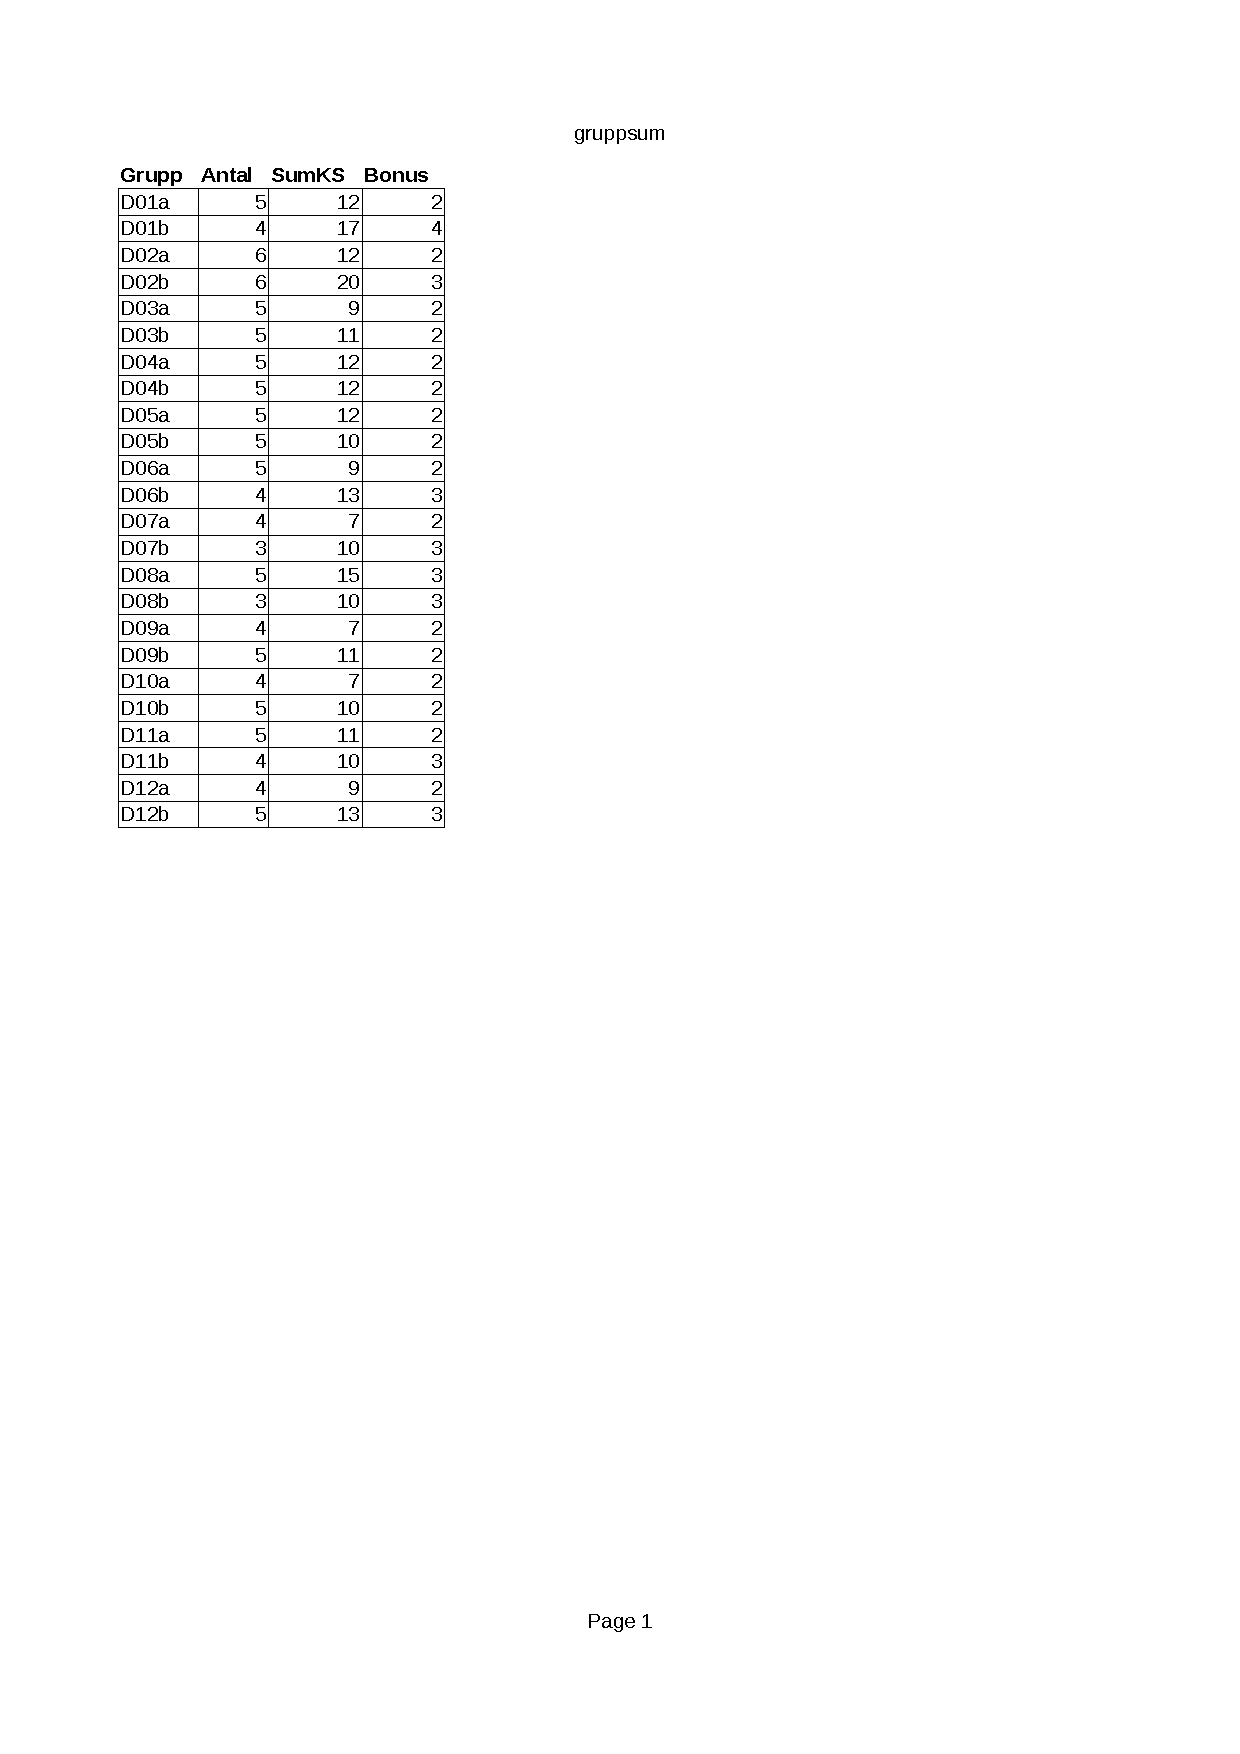
\includegraphics[clip, trim=0cm 1cm 3.2cm 2.5cm, width=0.9\textwidth]{../img/bonus-2016.pdf}

\columnbreak

\begin{itemize}
\pause
\item Bonus gäller vid första ordinarie tentatillfälle 
\pause
\item D07b och D08b har 3 st; \\ vill ni göra merge?

\end{itemize}
\end{multicols}
\end{Slide}

\Subsection{Specialundervisning}
\begin{Slide}{Specialundervisning}
Under vecka w09 och w10 (till att börja med) kommer vi att organisera \Emph{specialundervisning} under dessa \Alert{resurstider}:
\begin{itemize}
\item \Emph{Torsdag kl 8-10} i både \Alert{Falk} och \Alert{Val}  (Gustav, Valthor, Emil)
\item \Emph{Torsdag kl 10-12} i \Alert{Falk} (Maj)
\item OBS! Dessa rumtider är till för de som hade 0 eller 1 på kontrollskrivningen och som ansökt om specialundervisning via länk i speciell mejlinbjudan. 
\end{itemize}
\SlideFontSmall{Undantag: Om du har mer än 1 på kontrollskrivningen men inte alls har möjlighet att gå på någon annan resurstid än ovan är du också välkommen; anmäl då din situation till handledaren på plats och så får du vara med i gruppen och kan få svar på frågor etc. som vanligt.}
\end{Slide}
\fi












%!TEX encoding = UTF-8 Unicode
%!TEX root = ../lect-week09.tex

%%%


%\begin{Slide}{TODO: Begrepp att förklara}
%  Tänk igenom ordningen:
%  \begin{itemize}
%    \item java switch, scala match ... 
%  \end{itemize}
%\end{Slide}
%
%
%\begin{Slide}{Javas switch-sats}
%A switch in Java works with the byte, short, char, and int primitive data types. It also works with enumerated types (discussed in Enum Types), the String class, and a few special classes that wrap certain primitive types: Character, Byte, Short, and Integer
%\end{Slide}


\begin{Slide}{Javas switch-sats}

\begin{CodeSmall}[language=Java]
public class Switch {
    public static void main(String[] args) {
        String favorite = "selleri";
        if (args.length > 0) {
            favorite = args[0];
        }
        System.out.println("Din favoritgrönsak: " + favorite);
        char firstChar = Character.toLowerCase(favorite.charAt(0));
        System.out.print("Jag tycker ");
        switch (firstChar) {
        case 'g': 
            System.out.println("gurka är gott!");
            break;
        case 't': 
            System.out.println("tomat är gott!");
            break;
        case 'b': 
            System.out.println("brocolli är gott!");
            break;
        default:
            System.out.println(favorite + " är mindre gott...");
            break;
        }
    }
}
\end{CodeSmall}
\end{Slide}













%!TEX encoding = UTF-8 Unicode
%!TEX root = ../lect-week09.tex

%%%

\ifkompendium\else


\Subsection{Option}


\begin{Slide}{Hur hantera saknade värden?}\SlideFontSmall
Olika sätt att hantera saknade värden:
\begin{itemize}
\item Hitta på ett specialvärde: exempel -1 för icke nedtryckt sträng
\item \code{null} om \code{AnyRef}/\code{Object} (vanligt i Java, mkt ovanligt i Scala) 
\item Använd en samling och låt tom samling representera saknad värde: \\
\code{val grip = Vector(Vector(2), Vector(7), Vector(), Vector(3))}

\item \code{Option[T]} gemensam bastyp för: \\
  \code{None} som representerar \Alert{saknat värde}, och \\ \code{Some[T]} som representerar att \Emph{värde finns}
\end{itemize}
\end{Slide}

\begin{Slide}{En gemensam bastyp för ett värde som kanske saknas}\SlideFontSmall
\vspace{-0.5em}\begin{center}
\newcommand{\TextBox}[1]{\raisebox{0pt}[1em][0.5em]{#1}}
\tikzstyle{umlclass}=[rectangle, draw=black,  thick, anchor=north, text width=3cm, rectangle split, rectangle split parts = 3]
\begin{tikzpicture}[inner sep=0.5em]
\node [umlclass, rectangle split parts = 2, xshift=0cm, text width=3.5cm] (BaseType)  {
            \textit{\textbf{\centerline{\TextBox{\code{Option[A]}}}}}
            \nodepart[]{second}
            \TextBox{\code{def get: A}}\newline
            \TextBox{\code{def isEmpty: Boolean}}

        };
        
\node [umlclass, rectangle split parts = 1]  at (-2.5cm,-3.7cm) (SubType1) {
            \textbf{\centerline{\TextBox{\code{Some[A]}}}}
            % \nodepart[]{second} \TextBox{\code{val x: A}}
        };  
                
\node [umlclass, rectangle split parts = 1] at (2.5cm,-3.7cm) (SubType2)  {
            \textbf{\centerline{\TextBox{\code{None}}}}
        };        
\draw[umlarrow] (SubType1.north) -- ++(0,0.5) -| (BaseType.south);    
\draw[umlarrow] (SubType2.north) -- ++(0,0.5) -| (BaseType.south);            
\end{tikzpicture}
\end{center}
\end{Slide}


\begin{Slide}{Option för hantering av ev. saknade värden}\SlideFontSmall
Alla vill inte berätta för Facebook vad de har för kön. \\ Förbättra Facebooks kod med ett litet Scala-program:
\begin{Code}
trait Gender
case object Male   extends Gender
case object Female extends Gender

case class Person(name: String, gender: Option[Gender])
\end{Code}
\pause
\begin{REPL}
scala> val p1 = Person("Björn",  Some(Male))
scala> val p2 = Person("Sandra", Some(Female))
scala> val p3 = Person("Andro",  None)
scala> val g2 = p2.gender
scala> def show(g: Option[Gender]): String = g match {
         case Some(x) => x.toString
         case None    => "unknown"
       }
scala> show(g2)
scala> show(p3.gender)
scala> val ps = Vector(p1,p2,p3)
scala> ps.map(_.gender).map(show)
\end{REPL}
\end{Slide}

\begin{Slide}{Några smidiga metoder på \code{Option}}
getOrElse

map

foreach

isEmpty
\end{Slide}


\begin{Slide}{Några samlingsmetoder som ger en \code{Option}}
get på Map

headOption på Vector

find på Seq
\end{Slide}



\fi



%!TEX encoding = UTF-8 Unicode
%!TEX root = ../lect-week09.tex

%%%

\ifkompendium\else
\Subsection{Mer om \texttt{equals}}
\begin{Slide}{Fördjupning: Implementera \texttt{equals} med \texttt{match}}
Det visar sig att innehållslikhet är förvånansvärt komplicerat att implementera i samband med arv.
\begin{itemize}
\item Det enklare fallet: Gör övning \code{matching:12} och implementera \code{equals} för innehållslikhet utan arv. \\ En bra träning på att använda \code{match}!

\item Svårare: Gör fördjupningsövning \code{matching:19} om du vill se hur en \emph{komplett} \code{equals} ska se ut som funkar i alla lägen.

\end{itemize}

Det ingår inte på tentan att själv kunna implementera en genrellt fungerande \code{equals}. Men du ska förstå skillnaden mellan referenslikhet och innehållslikhet. Mer om \code{equals} i fortsättningkursen.
\end{Slide}
\fi












%!TEX encoding = UTF-8 Unicode
%!TEX root = ../lect-week09.tex

%%%


\ifkompendium\else

\Subsection{Undantag}
\begin{Slide}{Vad är ett undantag \Eng{exception}?}
Undantag representerar ett fel eller ett onormalt tillstånd som upptäcks under exekvering och som  behöver hanteras på särskilt sätt vid sidan av det normala exekveringsflödet. 

\vspace{1em}\href{https://sv.wikipedia.org/wiki/Undantagshantering}{sv.wikipedia.org/wiki/Undantagshantering}


\vspace{1em} Exempel på undantag:

\pause

\begin{itemize}
\item Indexering utanför vektorns indexgränser.

\item Läsning bortom filens slut.

\item Försök att öppna en fil som inte finns.

\item Minnet är slut.

\item Division med noll.

\item \code{"hej".toInt} resulterar i \\\code{java.lang.NumberFormatException}

\end{itemize}

\end{Slide}

\begin{Slide}{''Kasta'' dina egna undantag med \texttt{throw}}\SlideFontSmall
Man kan själv generera ett undantag med \code{throw}, vilket kallas att \Emph{kasta} ett undantag som (om det inte \Emph{fångas}), gör att exekveringen \Alert{avbryts}.


\begin{REPL}
scala> def pang = throw new Exception("PANG!")
pang: Nothing

scala> pang
java.lang.Exception: PANG!
  at .pang(<console>:11)
  ...
  
\end{REPL}
\pause
Olika sätt att hantera undantag: 
\begin{itemize}
\item Scala: Man kan använda ett \code{try ... catch}-uttryck och ge ett \Emph{värde} i händelse av undantag.
\item Java: Man kan använda en \code{try ... catch}-sats och \Alert{göra något} i händelse av undantag.
 
\item Scala: Man kan \Emph{kapsla in} ett undantag med \Emph{\texttt{scala.util.Try}} och förhindra att exekveringen avbryts. (Finns ej i Java; att föredra i Scala.)
\end{itemize}
\end{Slide}


\Subsection{\texttt{scala.util.Try}}

\begin{Slide}{En gemensam bastyp för något som kan misslyckas}\SlideFontSmall
\begin{Code}
import scala.util.{Try, Success, Failure}
\end{Code}

\vspace{-0.5em}\begin{center}
\newcommand{\TextBox}[1]{\raisebox{0pt}[1em][0.5em]{#1}}
\tikzstyle{umlclass}=[rectangle, draw=black,  thick, anchor=north, text width=3.0cm, rectangle split, rectangle split parts = 3]
\begin{tikzpicture}[inner sep=0.5em]
\node [umlclass, rectangle split parts = 2, xshift=0cm, text width=3.8cm] (BaseType)  {
            \textit{\textbf{\centerline{\TextBox{\code{Try[T]}}}}}
            \nodepart[]{second}
            \TextBox{\code{def get: T}}\newline
            \TextBox{\code{def isFailure: Boolean}}\newline
            \TextBox{\code{def isSuccess: Boolean}}
        };
        
\node [umlclass, rectangle split parts = 2, text width=2.2cm]  at (-2.5cm,-3.7cm) (SubType1) {
            \textbf{\centerline{\TextBox{\code{Success[T]}}}}
            \nodepart[]{second} \TextBox{\code{val value: T}}
        };  
                
\node [umlclass, rectangle split parts = 2, text width=4.2cm] at (2.5cm,-3.7cm) (SubType2)  {
            \textbf{\centerline{\TextBox{\code{Failure[T]}}}}
            \nodepart[]{second} \TextBox{\code{val exception: Throwable}}
        };        
\draw[umlarrow] (SubType1.north) -- ++(0,0.5) -| (BaseType.south);    
\draw[umlarrow] (SubType2.north) -- ++(0,0.5) -| (BaseType.south);            
\end{tikzpicture}
\end{center}
\end{Slide}

\begin{Slide}{Hantera undantag med \texttt{Try}}
\vspace{-0.5em}\begin{REPL}
scala> def pang = throw new Exception("PANG!")

scala> def kanskePang = if (math.random < 0.5) 42 else pang

scala> import scala.util.{Try, Success, Failure}

scala> def försök = Try { kanskePang }

scala> val xs = Vector.fill(15){försök}

scala> val trettonde = xs(13) match {
         case Success(value) => value
         case Failure(e) => println(e); -1
       }

scala> (xs(13).isSuccess, xs(13).isFailure)

scala> försök.foreach(println)

scala> försök.map(_ + 1)

scala> for (Success(x) <- xs) yield x
\end{REPL}
\end{Slide}

\begin{Slide}{Fördjupning: \texttt{try}-\texttt{catch}-uttryck}\SlideFontSmall
Man kan fånga undantag med ett \code{try ... catch}-uttryck:
\begin{Code}
def carola = try {
  if (math.random > 0.5) throw new Exception("stormvind")
  42
} catch { 
  case e: Exception =>
    println("Fångad av en " + e.getMessage)
    -1
}  
\end{Code}
\pause
\begin{REPL}
scala> Vector.fill(5)(carola)
Fångad av en stormvind
Fångad av en stormvind
Fångad av en stormvind
res0: scala.collection.immutable.Vector[Int] = Vector(-1, 42, 42, -1, -1)
\end{REPL}
\pause
\emph{Fördjupning:} \\ Gör övning 9-10 som visar hur man fångar undantag i Scala och Java. \\Mer om undantag i fortsättningskursen.
\end{Slide}


\fi







\Lecture{10}{Matriser, typparametrar}
%!TEX encoding = UTF-8 Unicode
%!TEX root = ../lect-week10.tex

%%%

\ifkompendium\else

\Subsection{Veckans labb: \texttt{maze}}
\begin{Slide}{Veckans labb: \texttt{maze}}\SlideFontSmall
Grunduppgift:
\begin{itemize}
\item Implementera en algoritm som hittar ut ur en labyrint.

\item En labyrint representeras av en \Emph{matris}, \\närmare bestämt en \Emph{vektor av vektorer} med  \Alert{booelska} värden: \\ \code{Vector[Vector[Boolean]]} 

\pause Där de två olika sanningsvärdena representerar följande:
\begin{itemize}\SlideFontSmall
\item \code{true} om det \Emph{finns en vägg} på en viss plats i matrisen
\item \code{false} om det \Alert{inte} finns en vägg på en viss plats i matrisen 

\end{itemize}
\pause
\item Använd enkel idé (som inte ger kortaste vägen): \\ Behåll vänster hand i kontakt med väggen och gå tills du når utgången.

\item Vad krävs av labyrinten för att detta ska fungera?  
\end{itemize}
\pause Extrauppgift:
\begin{itemize}
\item Generera slumpmässig labyrint 
\item Algoritmen (\emph{Prims algoritm}) är given i pseudokod
\end{itemize}

\end{Slide}

\begin{Slide}{Labyrint som booelsk matris}
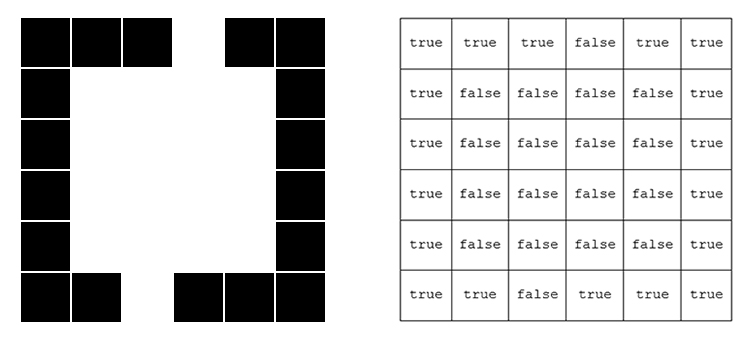
\includegraphics[width=1.0\textwidth]{../img/w09-lab/MazeAndMatrix.jpg}
\end{Slide}

\begin{Slide}{Slumpmässig labyrint}

\includegraphics[width=0.68\textwidth]{../img/w09-lab/RandomMaze.jpg}
\end{Slide}

\Subsection{Matriser}

\begin{Slide}{Vad är en matris?}\SlideFontSmall
\begin{multicols}{2}
\begin{itemize}
\item En \Emph{matris} inom \Alert{matematiken} innehåller \Emph{rader} med lika många tal och \Emph{kolumner} med lika många tal. 

\item En matris av dimension $m\times{}n$ har $m \cdot n$ stycken element. 

\end{itemize}

\columnbreak
\begin{itemize}
\item En matris $M_{2,5}$ ritas inom matematiken ofta så här:
\end{itemize}
\[
M=
  \begin{pmatrix}
    5 & 2 & 42 & 4 & 5 \\
    3 & 4 & 18 & 6 & 7
  \end{pmatrix}
\]

\begin{itemize}
\pause
\item Indexering inom matematiken sker från 1 (men oftast från 0 i datorprogram).

\item Vad har talet 42 för index i matrisen M ovan?
\end{itemize}
\end{multicols}
\end{Slide}

\begin{Slide}{En matris med array av arrayer}
Inom programmering används ordet \Emph{matris} ofta för att beteckna en \Alert{nästlade struktur} i två dimensioner, till exempel en instans av typen \code{Array[Array[Int]]}
\begin{REPL}
scala> val xss = Array(Array(5,2,42,4,5),Array(3,4,18,6,7))
xss: Array[Array[Int]] = Array(Array(5, 2, 42, 4, 5), Array(3, 4, 18, 6, 7))
\end{REPL}
\pause
Man indexerar i en nästlad sekvens med upprepad \code{apply}:
\begin{REPL}
scala> xss(0)(2)
res0: ???                   // Vad är typ och värde?

scala> xss.apply(0).apply(2)
res1: ???                   // Vad är typ och värde?

scala> xss(0)
res2: ???                   // Vad är typ och värde?
\end{REPL}

\end{Slide}

\begin{Slide}{En matris med array av arrayer}
Inom programmering används ordet \Emph{matris} ofta för att beteckna en \Alert{nästlade struktur} i två dimensioner, till exempel en instans av typen \code{Array[Array[Int]]}
\begin{REPL}
scala> val xss = Array(Array(5,2,42,4,5),Array(3,4,18,6,7))
xss: Array[Array[Int]] = Array(Array(5, 2, 42, 4, 5), Array(3, 4, 18, 6, 7))
\end{REPL}

Man indexerar i en nästlad sekvens med upprepad \code{apply}:
\begin{REPL}
scala> xss(0)(2)
res0: Int = 42

scala> xss.apply(0).apply(2)
res1: Int = 42

scala> xss(0)
res2: Array[Int] = Array(5, 2, 42, 4, 5)
\end{REPL}
\end{Slide}

\begin{Slide}{Uppdatering av en förändringsbar nästlad struktur}
Man kan förändra en array av arrayer ''på plats'' med tilldelning:
\begin{REPL}
scala> val xss = Array(Array(5,2,42,4,5),Array(3,4,18,6,7))

scala> xss(0)(0) = 100

scala> xss
res0: ???

scala> xss(0)(2) = xss(0)(2) - 1

scala> xss
res1: ???

scala> xss(1) = Array.fill(5)(-1)

scala> xss
res2: ???
\end{REPL}
\end{Slide}

\begin{Slide}{Uppdatering av en förändringsbar nästlad struktur}
Man kan förändra en array av arrayer ''på plats'' med tilldelning:
\begin{REPL}
scala> val xss = Array(Array(5,2,42,4,5),Array(3,4,18,6,7))

scala> xss(0)(0) = 100

scala> xss
res0: Array[Array[Int]]=Array(Array(100, 2, 42, 4, 5), Array(3, 4, 18, 6, 7))

scala> xss(0)(2) = xss(0)(2) - 1

scala> xss
res1: Array[Array[Int]]=Array(Array(100, 2, 41, 4, 5), Array(3, 4, 18, 6, 7))

scala> xss(1) = Array.fill(5)(-1)

scala> xss
res2: Array[Array[Int]]=Array(Array(100, 2, 41, 4, 5), Array(-1,-1,-1,-1,-1))
\end{REPL}
\end{Slide}

\begin{Slide}{Några olika sätt att skapa förändringsbara matriser}\SlideFontSmall
Det jobbiga, primitiva sättet:
\begin{REPL}
scala> val xs = new Array[Array[Int]](2)
xs: Array[Array[Int]] = Array(null, null)

scala> for (i <- xs.indices) {xs(i) = new Array[Int](5)}

scala> xs
res0: Array[Array[Int]] = Array(Array(0, 0, 0, 0, 0), Array(0, 0, 0, 0, 0))

scala> println(xs)
[[I@196a99d0
\end{REPL}
Enklare sätt:
\begin{REPL}
scala> val xs = Array.ofDim[Int](2,5)
xs: Array[Array[Int]] = Array(Array(0, 0, 0, 0, 0), Array(0, 0, 0, 0, 0))
\end{REPL}
Enklare och tydligare sätt, där initialvärdet anges explicit:
\begin{REPL}
scala> Array.fill(2,5)(0)
res37: Array[Array[Int]] = Array(Array(0, 0, 0, 0, 0), Array(0, 0, 0, 0, 0))
\end{REPL}

\end{Slide}

\begin{Slide}{Exempel på skapande av oföränderlig nästlad struktur}\SlideFontSmall
Om du kan beräkna initialvärde direkt, använd \code{Vector.fill}:\\
{\SlideFontTiny\code{def fill[A](n1: Int, n2: Int)(elem: => A): Vector[Vector[A]]}}
\begin{REPL}
scala> Vector.fill(2,5)(scala.util.Random.nextInt(6) + 1)
res0: 
  typ???
  värde???

\end{REPL}
Om du kan beräkna initialvärde ur index, använd \code{Vector.tabulate}:\\
{\SlideFontTiny\code{def tabulate[A](n1: Int, n2: Int)(f: (Int, Int) => A): Vector[Vector[A]]}}
\begin{REPL}
scala> Vector.tabulate(5,2)((x,y) => x + y + 1)
res1: 
  typ???
  värde???

\end{REPL}
\end{Slide}

\begin{Slide}{Exempel på skapande av oföränderlig nästlad struktur}\SlideFontSmall
Om du kan beräkna initialvärde direkt, använd \code{Vector.fill}:\\
{\SlideFontTiny\code{def fill[A](n1: Int, n2: Int)(elem: => A): Vector[Vector[A]]}}
\begin{REPL}
scala> Vector.fill(2,5)(scala.util.Random.nextInt(6) + 1)
res0: 
  scala.collection.immutable.Vector[scala.collection.immutable.Vector[Int]] = 
  Vector(Vector(1, 2, 6, 2, 1), Vector(1, 4, 3, 3, 2))

\end{REPL}
Om du kan beräkna initialvärde ur index, använd \code{Vector.tabulate}:\\
{\SlideFontTiny\code{def tabulate[A](n1: Int, n2: Int)(f: (Int, Int) => A): Vector[Vector[A]]}}
\begin{REPL}
scala> Vector.tabulate(5,2)((x,y) => x + y + 1)
res1: 
  scala.collection.immutable.Vector[scala.collection.immutable.Vector[Int]] = 
  Vector(Vector(1,2), Vector(2,3), Vector(3,4), Vector(4,5), Vector(5,	6))

\end{REPL}
\end{Slide}



\begin{Slide}{Uppdatering av en oföränderlig nästlad struktur}\SlideFontSmall
Uppdatering av endimensionell struktur med \code{xs.updated}:\\
{\SlideFontTiny\code{def updated[A](index: Int, elem: A): Vector[A]} }
\begin{REPL}
scala> var xs = Vector.tabulate(5)(x => x + 1)
xs: typ??? = värde???

scala> xs = xs.updated(1, 42)
xs: typ??? = värde???
\end{REPL}

Uppdatering av nästlad struktur i två dimensioner:
\begin{REPL}
scala> var xss = Vector.tabulate(2, 5)((x,y) => x + y + 1)
xss: 
  typ??? =
  värde???

scala> xss = xss.updated(0, xss(0).updated(1, 42))
xss: 
  typ??? =
  värde???
\end{REPL}

\end{Slide}



\begin{Slide}{Uppdatering av en oföränderlig nästlad struktur}\SlideFontSmall
Uppdatering av endimensionell struktur med \code{xs.updated}:\\
{\SlideFontTiny\code{def updated[A](index: Int, elem: A): Vector[A]} }
\begin{REPL}
scala> var xs = Vector.tabulate(5)(x => x + 1)
xs: scala.collection.immutable.Vector[Int] = Vector(1, 2, 3, 4, 5)

scala> xs = xs.updated(1, 42)
xs: scala.collection.immutable.Vector[Int] = Vector(1, 42, 3, 4, 5)
\end{REPL}

Uppdatering av nästlad struktur i två dimensioner:
\begin{REPL}
scala> var xss = Vector.tabulate(2, 5)((x,y) => x + y + 1)
xss: 
  scala.collection.immutable.Vector[scala.collection.immutable.Vector[Int]] = 
  Vector(Vector(1, 2, 3, 4, 5), Vector(2, 3, 4, 5, 6))

scala> xss = xss.updated(0, xss(0).updated(1, 42))
xss: 
  scala.collection.immutable.Vector[scala.collection.immutable.Vector[Int]] = 
  Vector(Vector(1, 42, 3, 4, 5), Vector(2, 3, 4, 5, 6))
\end{REPL}

\end{Slide}


\begin{Slide}{Iterera över nästlad struktur: for-sats}\SlideFontSmall
Iterera med nästlad for-sats:
\begin{REPL}
scala> val xss = Vector.tabulate(2,5)((x,y) => x + y + 1)

scala> for (???) { 
         for (???) {
           print(xss(i)(j) + " ")
         }
         println
       }

1 2 3 4 5 
2 3 4 5 6 
\end{REPL}
\end{Slide}

\begin{Slide}{Iterera över nästlad struktur: for-sats}\SlideFontSmall
Iterera med nästlad for-sats:
\begin{REPL}
scala> val xss = Vector.tabulate(2,5)((x,y) => x + y + 1)

scala> for (i <- xss.indices) { 
         for (j <- xss(i).indices) {
           print(xss(i)(j) + " ")
         }
         println
       }

1 2 3 4 5 
2 3 4 5 6 
\end{REPL}
\end{Slide}


\begin{Slide}{Övningsexempel: Yatzy}\SlideFontSmall
Skapa en funktion \code{roll} som ger utfallet av n st tärningskast:
\begin{REPL}
scala> import scala.util.Random

scala> def roll(n: Int): Vector[Int] = ???
\end{REPL}

Skapa en funktion \code{isYatzy} som ger \code{true} om alla utfall är lika:
\begin{REPL}
scala> def isYatzy(xs: Vector[Int]): Boolean = ???
\end{REPL}
Du kan anta att xs.length > 0\\
Tips: använd metoden xs.forall: \\
\code{def forall[A](p: A => Boolean): Boolean }
\end{Slide}


\begin{Slide}{Övningsexempel: Yatzy}\SlideFontSmall
Skapa en funktion \code{roll} som ger utfallet av n st tärningskast:
\begin{REPL}
scala> import scala.util.Random

scala> def roll(n: Int): Vector[Int] = Vector.fill(n)(Random.nextInt(6) + 1)
\end{REPL}

Skapa en funktion \code{isYatzy} som ger \code{true} om alla utfall är lika:
\begin{REPL}
scala> def isYatzy(xs: Vector[Int]): Boolean = xs.forall(x => x == xs(0))
\end{REPL}
Du kan anta att xs.length > 0\\
Tips: använd metoden xs.forall: \\
\code{def forall[A](p: A => Boolean): Boolean }
\end{Slide}

\begin{Slide}{Iterera över nästlad struktur: for-sats}\SlideFontSmall
Iterera med nästlad for-sats: (vad har xss för typ?)
\begin{REPL}
scala> val xss = Vector.fill(100)(roll(5))

scala> for (???) { 
         for (???) {
           print(s"($i)($j) == " + xss(i)(j) + " ")
         }
         println(isYatzy(???))
       }

(0)(0) == 5 (0)(1) == 3 (0)(2) == 4 (0)(3) == 1 (0)(4) == 3 false
(1)(0) == 3 (1)(1) == 3 (1)(2) == 6 (1)(3) == 3 (1)(4) == 1 false
(2)(0) == 3 (2)(1) == 4 (2)(2) == 2 (2)(3) == 2 (2)(4) == 1 false
(3)(0) == 5 (3)(1) == 2 (3)(2) == 6 (3)(3) == 5 (3)(4) == 1 false
(4)(0) == 4 (4)(1) == 6 (4)(2) == 4 (4)(3) == 1 (4)(4) == 4 false
(5)(0) == 3 (5)(1) == 4 (5)(2) == 6 (5)(3) == 5 (5)(4) == 1 false
(6)(0) == 4 (6)(1) == 6 (6)(2) == 2 (6)(3) == 2 (6)(4) == 6 false
(7)(0) == 2 (7)(1) == 5 (7)(2) == 3 (7)(3) == 6 (7)(4) == 2 false
(8)(0) == 4 (8)(1) == 4 (8)(2) == 6 (8)(3) == 1 (8)(4) == 4 false
(9)(0) == 3 (9)(1) == 3 (9)(2) == 3 (9)(3) == 3 (9)(4) == 3 true
(10)(0) == 1 (10)(1) == 2 (10)(2) == 4 (10)(3) == 3 (10)(4) == 3 false
(11)(0) == 6 (11)(1) == 5 (11)(2) == 4 (11)(3) == 1 (11)(4) == 5 false
(12)(0) == 3 (12)(1) == 6 (12)(2) == 6 (12)(3) == 4 (12)(4) == 2 false
\end{REPL}
\end{Slide}

\begin{Slide}{Iterera över nästlad struktur: for-sats}\SlideFontSmall
Iterera med nästlad for-sats: (xss är en \code{Vector[Vector[Int]]})
\begin{REPL}
scala> val xss = Vector.fill(100)(roll(5))

scala> for (i <- xss.indices) { 
         for (j <- xss(i).indices) {
           print(s"($i)($j) == " + xss(i)(j) + " ")
         }
         println(isYatzy(xss(i)))
       }

(0)(0) == 5 (0)(1) == 3 (0)(2) == 4 (0)(3) == 1 (0)(4) == 3 false
(1)(0) == 3 (1)(1) == 3 (1)(2) == 6 (1)(3) == 3 (1)(4) == 1 false
(2)(0) == 3 (2)(1) == 4 (2)(2) == 2 (2)(3) == 2 (2)(4) == 1 false
(3)(0) == 5 (3)(1) == 2 (3)(2) == 6 (3)(3) == 5 (3)(4) == 1 false
(4)(0) == 4 (4)(1) == 6 (4)(2) == 4 (4)(3) == 1 (4)(4) == 4 false
(5)(0) == 3 (5)(1) == 4 (5)(2) == 6 (5)(3) == 5 (5)(4) == 1 false
(6)(0) == 4 (6)(1) == 6 (6)(2) == 2 (6)(3) == 2 (6)(4) == 6 false
(7)(0) == 2 (7)(1) == 5 (7)(2) == 3 (7)(3) == 6 (7)(4) == 2 false
(8)(0) == 4 (8)(1) == 4 (8)(2) == 6 (8)(3) == 1 (8)(4) == 4 false
(9)(0) == 3 (9)(1) == 3 (9)(2) == 3 (9)(3) == 3 (9)(4) == 3 true
(10)(0) == 1 (10)(1) == 2 (10)(2) == 4 (10)(3) == 3 (10)(4) == 3 false
(11)(0) == 6 (11)(1) == 5 (11)(2) == 4 (11)(3) == 1 (11)(4) == 5 false
(12)(0) == 3 (12)(1) == 6 (12)(2) == 6 (12)(3) == 4 (12)(4) == 2 false
\end{REPL}
\end{Slide}


\begin{Slide}{Iterera över nästlad struktur med nästlad foreach}\SlideFontSmall
Iterera med nästlad foreach-sats:
\begin{REPL}
scala> val xss = Vector.tabulate(2,5)((x,y) => x + y + 1)

xss.foreach{ xs => ??? ; println }

1 2 3 4 5 
2 3 4 5 6 
\end{REPL}
\end{Slide}


\begin{Slide}{Iterera över nästlad struktur med nästlad foreach}\SlideFontSmall
Iterera med nästlad foreach-sats:
\begin{REPL}
scala> val xss = Vector.tabulate(2,5)((x,y) => x + y + 1)

xss.foreach{ xs => xs.foreach{ x => print(x + " ") }; println }

1 2 3 4 5 
2 3 4 5 6 
\end{REPL}
\end{Slide}


\begin{Slide}{Nästlade for-uttryck}\SlideFontSmall
Iterera med \Emph{nästlad for-yield}:\\
%Statisk typ: \code{IndexedSeq[IndexedSeq[[Int]]} \\
%Dynamisk typ: \code{Vector[Vector[[Int]]}
 
\begin{REPL}
scala> val xss = for (i <- 1 to 2) yield { 
                   for (j <- 1 to 5) yield i + j + 1
                 }
xss: 
  scala.collection.immutable.IndexedSeq[
    scala.collection.immutable.IndexedSeq[Int]] = 
      ???

\end{REPL}
Om man skriver så här får man en endimensionell struktur:
\begin{REPL}
scala> val xs = for (i <- 1 to 2; j <- 1 to 5) yield i + j + 1
xs: 
  scala.collection.immutable.IndexedSeq[Int] = 
    ???

\end{REPL}
\end{Slide}

\begin{Slide}{Nästlade for-uttryck}\SlideFontSmall
Iterera med \Emph{nästlad for-yield}:\\
\begin{REPL}
scala> val xss = for (i <- 1 to 2) yield { 
                   for (j <- 1 to 5) yield i + j + 1
                 }
xss: 
  scala.collection.immutable.IndexedSeq[
    scala.collection.immutable.IndexedSeq[Int]] = 
      Vector(Vector(3, 4, 5, 6, 7), Vector(4, 5, 6, 7, 8))

\end{REPL}
Om man skriver så här får man en endimensionell struktur:
\begin{REPL}
scala> val xs = for (i <- 1 to 2; j <- 1 to 5) yield i + j + 1
xs: 
  scala.collection.immutable.IndexedSeq[Int] = 
    Vector(3, 4, 5, 6, 7, 4, 5, 6, 7, 8)

\end{REPL}
\end{Slide}



\begin{Slide}{Nästlade map-uttryck}\SlideFontSmall
Iterera med \Emph{nästlade map-uttryck}:\\
\begin{REPL}
scala> val xss = (1 to 2).map(i => (1 to 5).map(j => i + j + 1))
xss: 
  scala.collection.immutable.IndexedSeq[
    scala.collection.immutable.IndexedSeq[Int]] = 
      ???
\end{REPL}
\end{Slide}

\begin{Slide}{Nästlade map-uttryck}\SlideFontSmall
Iterera med \Emph{nästlade map-uttryck}:\\
\begin{REPL}
scala> val xss = (1 to 2).map(i => (1 to 5).map(j => i + j + 1))
xss: 
  scala.collection.immutable.IndexedSeq[
    scala.collection.immutable.IndexedSeq[Int]] = 
      Vector(Vector(3, 4, 5, 6, 7), Vector(4, 5, 6, 7, 8))
\end{REPL}
\end{Slide}




\begin{Slide}{Matris som Array med Array med heltal i Java}\SlideFontTiny
\begin{CodeSmall}[language=Java]
public class ArrayMatrix {

    public static void showMatrix(int[][] m){
        System.out.println("\n--- showMatrix ---");
        for (int row = 0; row < m.length; row++){
            for (int col = 0; col < m[row].length; col++) {
                System.out.print("[" + row + "]");
                System.out.print("[" + col + "] = ");
                System.out.print(m[row][col] + "; ");
            }
            System.out.println();
        }
    }
    
    public static void main(String[] args) {
        int[][] xss = new int[10][5];
        showMatrix(xss);
    }
}
\end{CodeSmall}
\pause
Övning: skriv en metod \code{fillRnd} som fyller en heltalsmatris med slumptal 1 till n: 
\pause
\jcode|public static void fillRnd(int[][] m, int n){ /* ??? */ }| \\
\pause
Tips: använd en nästlad for-sats och: \\ 
\jcode{(int) (Math.random * n + 1)   // (int) motsvarar Scalas asInstanceOf[Int]}

\end{Slide}

\begin{Slide}{Om veckans övningar}\SlideFontSmall
\begin{itemize}
\item Träna på att iterera i nästlade strukurer

\item Fortsätt jobba med Yatzy-exemplet

\item Övning 2f) ger träning i att skapa en \Emph{imperativ} algoritm: \\ 
lös \code{isYatzy} med \code{while}-sats (kunde varit del av en tenta...)

\item Extrauppgiften 7 är en bra träning på matriser där du ska bygga ett enkelt yatzy-spel i terminalen (kunde varit del av en tenta...)

\item Uppgift 3 är en förberedelse inför nästa veckas labb: \code{survey} då vi ska analysera enkäter och kombinera matriser \& registrering \& sortering.

\end{itemize}
\end{Slide}

\begin{Slide}{Övning 3, utgör början på labb \code{survey}}\SlideFontSmall

\begin{ScalaSpec}{Table}
object Table {
  /** Creates a new Table from fileName with columns split by sep */
  def fromFile(fileName: String, separator: Char = ';'): Table = ???
}
case class Table(
  data: Vector[Vector[String]], 
  headings: Vector[String], 
  sep: String){
  /** A 2-tuple with (number of rows, number of columns) in data */
  val dim: (Int, Int) = ???

  /** The element in row r an column c of data, counting from 0 */
  def apply(r: Int, c: Int): String = ???

  /** The row-vector r in data, counting from 0 */
  def row(r: Int): Vector[String]= ???

  /** The column-vector c in data, counting from 0 */
  def col(c: Int): Vector[String] = ???

  /** A map from heading to index counting from 0 */
  lazy val indexOfHeading: Map[String, Int] = ???

  /** The column-vector with heading h in data */
  def col(h: String): Vector[String] = ???

  /** A vector with the distinct, sorted values of col with heading h */ 
  def values(h: String): Vector[String] = ???

  /** Headings and data with columns separated by sep */
  override lazy val toString: String = ???
}
\end{ScalaSpec}
\end{Slide}



\fi












%!TEX encoding = UTF-8 Unicode
%!TEX root = ../lect-week10.tex

\ifkompendium\else

\Subsection{Typparametrar}

\begin{Slide}{Vad är en typparameter?}\SlideFontSmall
\begin{itemize}
\item En \Emph{typparameter} gör det möjligt att ge ett \Emph{typargument}
\item En \Emph{fri} typparameter kan bindas till vilken typ som helst 
\item Bindingen sker vid \Alert{kompileringstid}
\item En typparameter är \Emph{fri} om den \Alert{inte} fått något värde i omslutande deklarationer, annars \Emph{bunden}.
\end{itemize}
Exempel: \Emph{generisk} metod:
\begin{Code}
def tnirp[A](x: A):Unit = println(x.toString.reverse)
\end{Code}
\pause
Exempel: \Emph{generisk} klass:
\begin{Code}
class Cell[A](var value: A){
  override def toString = s"Cell($value)"
  def concat(x: A): Cell[String] = new Cell(value.toString + x)   // A bunden
  def tnirp[B](x: B): Unit = println(x.toString.reverse)          // B fri
} 
\end{Code}
\pause
\begin{itemize}
\item \Alert{Skuggning kan förekomma}: Om \code{tnirp} i \code{Cell} hade använt namnet A på sin typparameter hade den \Emph{skuggat} klassens typparameter och blivit en ny fri typparameter.
\end{itemize}

\end{Slide}

\begin{Slide}{Exempel: Generisk funktion}
Vad händer här?
\begin{REPL}

scala> def skrikBaklänges(x: T): String = x.toString.toUpperCase.reverse
???



scala> def skrikBaklänges[T](x: T): String = x.toString.toUpperCase.reverse

scala> skrikBaklänges("gurka är gott")
res0: ???

\end{REPL}
\end{Slide}

\begin{Slide}{Exempel: Generisk funktion}
Vad händer här?
\begin{REPL}

scala> def skrikBaklänges(x: T): String = x.toString.toUpperCase.reverse
<console>:11: error: not found: type T
       def skrikBaklänges(x: T): String = x.toString.toUpperCase.reverse
                             ^

scala> def skrikBaklänges[T](x: T): String = x.toString.toUpperCase.reverse

scala> skrikBaklänges("gurka är gott")
res0: ???
\end{REPL}
\end{Slide}

\begin{Slide}{Exempel: Generisk funktion}
Vad händer här?
\begin{REPL}

scala> def skrikBaklänges(x: T): String = x.toString.toUpperCase.reverse
<console>:11: error: not found: type T
       def skrikBaklänges(x: T): String = x.toString.toUpperCase.reverse
                             ^

scala> def skrikBaklänges[T](x: T): String = x.toString.toUpperCase.reverse

scala> skrikBaklänges("gurka är gott")
res0: String = TTOG RÄ AKRUG
\end{REPL}
\end{Slide}


\begin{Slide}{Exempel: Generisk case-klass}
\vspace{-0.5em}\begin{REPL}
scala> def skrikBaklänges[T](x: T): String = x.toString.toUpperCase.reverse

scala> case class Grönsak(whatever: A)
???
 
 
scala> case class Grönsak[A](whatever: A)

scala> Grönsak("gurka")
res1: ???

scala> skrikBaklänges(Grönsak(42))
res2: ???

scala> Grönsak[Int](42)
res3: ???

scala> Grönsak[String](42)
???



                       ^
\end{REPL}
\end{Slide}

\begin{Slide}{Exempel: Generisk case-klass}
\vspace{-0.5em}\begin{REPL}
scala> def skrikBaklänges[T](x: T): String = x.toString.toUpperCase.reverse

scala> case class Grönsak(whatever: A)
<console>:11: error: not found: type A
       case class Grönsak(whatever: A)
                                    ^
scala> case class Grönsak[A](whatever: A)

scala> Grönsak("gurka")
res1: Grönsak[String] = Grönsak(gurka)

scala> skrikBaklänges(Grönsak(42))
res2: String = )24(KASNÖRG

scala> Grönsak[Int](42)
res3: Grönsak[Int] = Grönsak(42)

scala> Grönsak[String](42)
<console>:14: error: type mismatch;
 found   : Int(42)
 required: String
       Grönsak[String](42)
                       ^
\end{REPL}
\end{Slide}

\begin{Slide}{Fallgrop: likhet av array}
\begin{REPL}
scala> Vector.fill(5)(42) == Vector.fill(5)(42)
res0: ???

scala> Array.fill(5)(42) == Array.fill(5)(42)
res1: ???
\end{REPL}
\end{Slide}


\begin{Slide}{Fallgrop: likhet av array}
\begin{REPL}
scala> Vector.fill(5)(42) == Vector.fill(5)(42)
res0: Boolean = true

scala> Array.fill(5)(42) == Array.fill(5)(42)
res1: Boolean = false  // AAAARRGH!!! :(
\end{REPL}
Primitiva arrayer har en equals-metod som ger referenslikhet, \Alert{inte} innehållslikhet.
\end{Slide}

\begin{Slide}{Kolla likhet av array-matris med nästlad while}
\begin{REPL}
scala> def isEqual(xss: Array[Array[Int]], yss: Array[Array[Int]]) = {
         var i = 0
         var allEqual = true
         while (???) {
           var j = 0
           while (???) {
             if (xss(i)(j) != yss(i)(j)) ???
             j += 1
           }
           i += 1
         }
         allEqual
       }

scala> val (xss, yss) = (Array.fill(5,2)(42), Array.fill(5,2)(42))

scala> isEqual(xss, yss)

scala> yss(4)(1) = 0

scala> isEqual(xss, yss)
\end{REPL}
\end{Slide}



\begin{Slide}{Kolla likhet av array-matris med nästlad while}
\begin{REPL}
scala> def isEqual(xss: Array[Array[Int]], yss: Array[Array[Int]]) = {
         var i = 0
         var allEqual = true
         while (i < xss.length && allEqual) {
           var j = 0
           while (j < xss(i).length && allEqual) {
             if (xss(i)(j) != yss(i)(j)) allEqual = false
             j += 1
           }
           i += 1
         }
         allEqual
       }

scala> val (xss, yss) = (Array.fill(5,2)(42), Array.fill(5,2)(42))

scala> isEqual(xss, yss)

scala> yss(4)(1) = 0

scala> isEqual(xss, yss)
\end{REPL}
\end{Slide}


\begin{Slide}{Fördjupning: Fallgrop typradering \Eng{type erasure}}\SlideFontSmall
Informationen om typerna i typparametrar raderas innan kodgenerering av prestandaskäl och \Alert{typinformationen finns ej vid runtime}.
\vspace{-0.25em}\begin{REPL}
scala> val xs = Vector(1,2,3)
xs: scala.collection.immutable.Vector[Int] = Vector(1, 2, 3)

scala> val ys = xs.map(_.toDouble)
ys: scala.collection.immutable.Vector[Double] = Vector(1.0, 2.0, 3.0)

scala> def hasDoubles[T](xs: Vector[T]): Boolean = xs match {
         case _: Vector[Int] => false
         case _: Vector[Double] => true
       }

<console>:13: warning: ???


                        ^
<console>:14: warning: ???


                        ^
<console>:14: warning: ???
\end{REPL}
\end{Slide}


\begin{Slide}{Fördjupning: Fallgrop typradering \Eng{type erasure}}\SlideFontSmall
Informationen om typerna i typparametrar raderas innan kodgenerering av prestandaskäl och \Alert{typinformationen finns ej vid runtime}.
\vspace{-0.25em}\begin{REPL}
scala> val xs = Vector(1,2,3)
xs: scala.collection.immutable.Vector[Int] = Vector(1, 2, 3)

scala> val ys = xs.map(_.toDouble)
ys: scala.collection.immutable.Vector[Double] = Vector(1.0, 2.0, 3.0)

scala> def hasDoubles[T](xs: Vector[T]): Boolean = xs match {
         case _: Vector[Int] => false
         case _: Vector[Double] => true
       }

<console>:13: warning: non-variable type argument Int in type pattern scala.collection.immutable.Vector[Int]
is unchecked since it is eliminated by erasure
                case _: Vector[Int] => false
                        ^
<console>:14: warning: non-variable type argument Double in type pattern scala.collection.immutable.Vector[Int]
is unchecked since it is eliminated by erasure
                case _: Vector[Double] => true
                        ^
<console>:14: warning: unreachable code: case _: Vector[Double] => true
\end{REPL}
\end{Slide}

\begin{Slide}{Fördjupning: Dynamisk typtest vid typradering}\SlideFontSmall
Typtest vid körtid med nästlad matchning:
\begin{REPL}
scala> def hasDoubles2[T](xs: Vector[T]): Boolean = xs match {
         case x +: xs => x match { 
           case _: Double => true
           case _ => false
         }  
         case _ => false
       }

scala> hasDoubles2(Vector(1.0))    // funkar!
\end{REPL}

Typtest vid körtid med match och gard med \code{isInstanceOf}:
\begin{REPL}
       
scala> def hasDoubles3[T](xs: Vector[T]): Boolean = xs match {
         case x +: xs if x.isInstanceOf[Double] => true
         case _ => false
       }

scala> hasDoubles3(Vector(1.0))    // funkar!
       
       
\end{REPL}
\end{Slide}


\begin{Slide}{Typparametrar på tentan?}
\begin{itemize}
\item Det ingår att kunna använda färdiga generiska strukturer med specifik typer, t.ex. \code{Vector[Int]}

\item Det ingår att kunna skapa strukturer med specifika typparametrar, t.ex. en case-klass som tar en vektor med en specifik typ:\\
\code{case class X(x: Vector[Int])}



\item Det ingår \Alert{inte} på tentan att kunna skapa generiska metoder eller klasser, t.ex.: \\
\code{def f[T](x: Vector[T]): Vector[T] = ???} \\
Mer om generiska strukturer fortsättningskursen!
\end{itemize}
\end{Slide}

\fi








\Lecture{11}{Sökning, sortering}
%!TEX encoding = UTF-8 Unicode
%!TEX root = ../lect-week11.tex

%%%

\ifkompendium\else

\Subsection{Veckans labb: \texttt{survey2}}
\begin{Slide}{Veckans labb: \texttt{survey2}}\SlideFontTiny
\begin{minipage}{0.65\textwidth}
Nya version 2 av labben är enklare och kräver ej att du implementerar parsning av \code{args}. Välj själv vilken du gör.

\vspace{0.5em}
\Emph{Förberedelse:}
\begin{itemize}
\item Studera givna koden: {\SlideFontTiny \href{https://github.com/lunduniversity/introprog/tree/master/workspace/w10_survey2/src/main/scala/stats}{workspace/w10\_survey2}}
\item Fyll i denna enkät:
\\{\SlideFontTiny \url{https://goo.gl/forms/hC6JK2UQXVpbGECc2}} 
\end{itemize}

\Emph{Grunduppgift:}
\begin{itemize}
\item Implementera en klass \code{Table} för hantering av strängmatriser med rubrikrad från kolumnsepararade textfiler.
\item Öva på att kombiner matriser, sortering, registrering för att räkna statistik.
\item Använda inbyggda sorteringsfunktioner: \\\code{sortBy} och \code{sortWith}
\item Implementera din egen sortering från scratch.
\end{itemize}
\Emph{Extrauppgift:}
\begin{itemize}
\item Implementera stapeldiagram.
\end{itemize}
\end{minipage}
\hfill\begin{minipage}{0.27\textwidth}
\centering
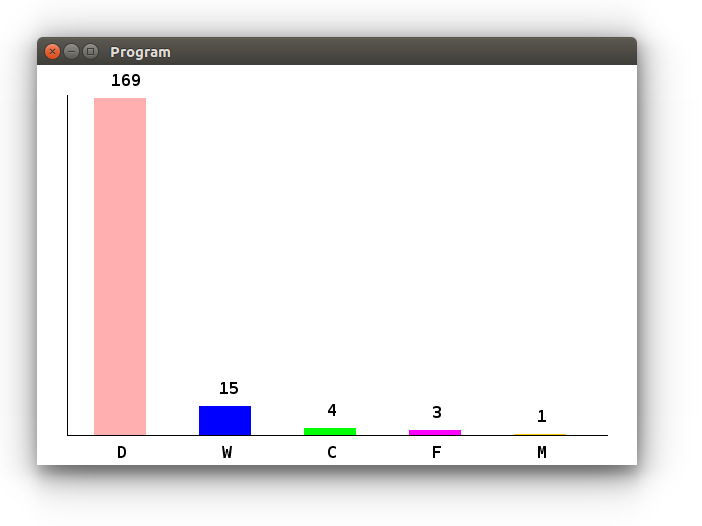
\includegraphics[width=0.9\textwidth]{../img/survey/bar}

\vspace{2em}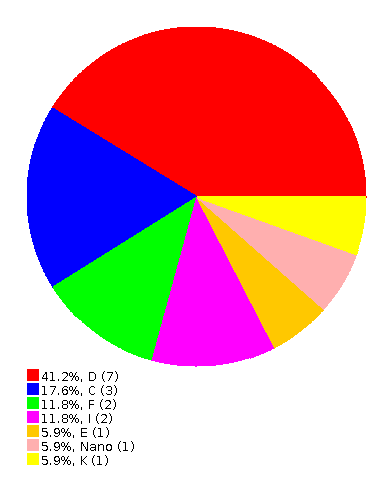
\includegraphics[width=0.7\textwidth]{../img/survey/pie}
\end{minipage}
\end{Slide}


\fi












%!TEX encoding = UTF-8 Unicode
%!TEX root = ../lect-week11.tex

%%%

\ifkompendium\else
\subsection{Repetition: Vad är en algoritm?}
\begin{Slide}{Repetition: Vad är en algoritm? }\SlideFontTiny
\pause En \href{https://sv.wikipedia.org/wiki/Algoritm}{algoritm} är en stegvis beskrivning av hur man löser ett problem. \\ 
Exempel: SWAP, MIN, Registrering, Sökning, Sortering \\
\pause\vspace{0.5em}
Problemlösningsprocessens olika steg (inte nödvändigtvis i denna ordning): 
\begin{itemize}
\item Dela upp problemet i enklare delproblem och sätt samman.
\item Finns redan färdig lösning på (del)problem?
\item Formulera (del)\Emph{problemet} och ange tydligt indata och utdata: \\ exempel MIN: indata: sekvens av heltal; utdata: minsta talet
\item Kom på en \Emph{lösningsidé}: (kan  vara mycket klurigt och svårt) \\ exempel MIN: iterera över talen och håll reda på ''minst hittills''
\item Formulera en \Emph{stegvis beskrivning} som löser problemet: \\ exempel: pseudo-kod med sekvens av instruktioner
\item Implementera en \Emph{körbar lösning} i ''riktig'' kod: \\ exempel: en Scala-metod i en klass eller i ett singelobjekt
\item Har algoritmen acceptabel komplexitet i förhållande till tids- och minneskrav?
\end{itemize}
\pause Det krävs ofta \Emph{kreativitiet} i stegen ovan  -- även i att \Emph{känna igen} problemet!\\
Simpelt exempel: Du stöter på problemet MAX och ser likheten med MIN.\\
\pause\vspace{0.5em}\Emph{Övning}: Diskutera hur du löser detta problem i relation till stegen ovan: \\
\emph{Att räkna antalet förekomster av olika unika ord i en textsträng.} 
\end{Slide}


\fi












%!TEX encoding = UTF-8 Unicode
%!TEX root = ../lect-week11.tex

%%%

\ifkompendium\else

\Subsection{Jämföra strängar}
\begin{Slide}{Jämföra strängar}\SlideFontSmall
\begin{itemize}
\item 
\end{itemize}

\end{Slide}


\fi












%!TEX encoding = UTF-8 Unicode
%!TEX root = ../lect-week11.tex

%%%

\ifkompendium\else

\Subsection{Sökning}
\begin{Slide}{Sökning}\SlideFontSmall

\begin{itemize}
\item \Emph{Sökning} återkommer i många skepnader: \\ i en datastruktur, vilken det än må vara, vill man ofta kunna \\ \Emph{hitta ett element med en viss egenskap}. 

\pause
Några färdiga linjärsökningar i Scalas standardbibliotek:

\begin{REPL}
scala> Vector("gurka","tomat","broccoli").indexOf("tomat")
res0: Int = 1

scala> Vector("gurka","tomat","broccoli").indexWhere(_.contains("o"))
res1: Int = 1

scala> Vector("gurka","tomat","broccoli").find(_.contains("o"))
res2: Option[String] = Some(tomat)
\end{REPL}

\pause
\item Sökning efter ett visst index i en sekvens:

\begin{itemize}\SlideFontTiny
\item Indata: en sekvens och ett \Emph{sökkriterium}
\item Utdata: index för första eftersökta element, annars -1 
\end{itemize}

\pause
\item Två typiska varianter av sökning i en sekvens:
\begin{itemize}\SlideFontTiny
\item Linjärsökning: börja från början och sök tills ett eftersökt element är funnet
\item Binärsökning: antag sorterad sekvensen; börja i mitten, välj rätt halva ...
\end{itemize}
\end{itemize}
\end{Slide}

\Subsection{Linjärsökning}

\begin{Slide}{Linjärsökning: hitta index för elementet 42}
Skriv pseudokod för:\\ \code{def indexOf42(xs: Vector[Int]): Int = ???}
\pause
\begin{Code}
def indexOf42(xs: Vector[Int]): Int = {
  var i = /* index för första elementet */
  var found = false
  while (!found && /* index inom indexgräns */) {
    if (/* element på plats i är 42 */) found = true 
    else i = /* nästa index */
  }
  if (/* hittat */) i else -1
} 
\end{Code}
\end{Slide}

\begin{Slide}{Linjärsökning: hitta index för elementet 42}
Implementera:\\ \code{def indexOf42(xs: Vector[Int]): Int = ???}
\pause
\begin{Code}
def indexOf42(xs: Vector[Int]): Int = {
  var i = 0
  var found = false
  while (!found && i < xs.length) {
    if (xs(i) == 42) found = true 
    else i += 1
  }
  if (found) i else -1
} 
\end{Code}
\end{Slide}

\begin{Slide}{Linjärsökning: hitta index för elementet x}
Implementera:\\ \code{def indexOf(xs: Vector[Int], x: Int): Int = ???}
\pause
\begin{Code}
def indexOf(xs: Vector[Int], x: Int): Int = {
  var i = 0
  var found = false
  while (!found && i < xs.length) {
    if (xs(i) == x) found = true 
    else i += 1
  }
  if (found) i else -1
} 
\end{Code}
\end{Slide}

\begin{Slide}{Linjärsökning: hitta index för elementet p(x)}\SlideFontSmall
Implementera:\\ \code{def indexWhere(xs: Vector[Int], p: Int => Boolean): Int = ???}
\pause
\begin{Code}
def indexWhere(xs: Vector[Int], p: Int => Boolean): Int = {
  var i = 0
  var found = false
  while (!found && i < xs.length) {
    if (p(xs(i))) found = true 
    else i += 1
  }
  if (found) i else -1
} 
\end{Code}
\end{Slide}

\begin{Slide}{Linjärsökning: generalisera till godtycklig typ}\SlideFontSmall
Implementera:\\ \code{def indexWhere[T](xs: Vector[T], p: T => Boolean): Int = ???}
\pause
\begin{Code}
def indexWhere[T](xs: Vector[T], p: T => Boolean): Int = {
  var i = 0
  var found = false
  while (!found && i < xs.length) {
    if (p(xs(i))) found = true 
    else i += 1
  }
  if (found) i else -1
} 
\end{Code}
\end{Slide}

\begin{Slide}{Linjärsökning: generalisera till godtycklig typ}\SlideFontSmall
Typinferensen fungerar bättre om stegad funktion:\\ 
\code{def indexWhere[T](xs: Vector[T])(p: T => Boolean): Int}
\begin{Code}
def indexWhere[T](xs: Vector[T])(p: T => Boolean): Int = {
  var i = 0
  var found = false
  while (!found && i < xs.length) {
    if (p(xs(i))) found = true 
    else i += 1
  }
  if (found) i else -1
} 
\end{Code}
\end{Slide}


\begin{Slide}{Linjärsökning: generalisera till godtycklig sekvens}\SlideFontSmall
Implementera:\\ \code{def indexWhere[T](xs: Seq[T])(p: T => Boolean): Int = ???}
\pause
\begin{Code}
def indexWhere[T](xs: Seq[T])(p: T => Boolean): Int = {
  var i = 0
  var found = false
  while (!found && i < xs.length) {
    if (p(xs(i))) found = true 
    else i += 1
  }
  if (found) i else -1
} 
\end{Code}
\end{Slide}

\begin{Slide}{Linjärsökning: generalisera till godtycklig sekvens}\SlideFontSmall
Implementera:\\ \code{def find[T](xs: Seq[T])(p: T => Boolean): Option[T] = ???}
\pause
\begin{Code}
def find[T](xs: Seq[T])(p: T => Boolean): Option[T] = {
  var i = 0
  var found = false
  while (!found && i < xs.length) {
    if (p(xs(i))) found = true 
    else i += 1
  }
  if (found) Some(xs(i)) else None
} 
\end{Code}
\end{Slide}

\Subsection{Binärsökning}

\begin{Slide}{Binärsökning: snabbare men kräver sorterad sekvens}
\begin{REPL}[basicstyle=\color{white}\ttfamily\SlideFontSize{6.5}{8}]
scala> val enMiljon = 1000000

scala> val xs = Array.tabulate(enMiljon)(i => i + 1)   // sorterad

scala> xs(enMiljon - 1)
res0: Int = 1000000

scala> timed { xs.indexOf(enMiljon) }        // linjärsökning
res42: (Double, Int) = (0.016622994,999999)

scala> import scala.collection.Searching._  // ger tillgång till metoden search
import scala.collection.Searching._

scala> timed { xs.search(enMiljon) }        // binärsökning
res54: (Double, collection.Searching.SearchResult) = (2.45691E-4,Found(999999))

\end{REPL}
\pause
Citat från scaladoc för \code{search}:\\
''The sequence \Alert{should be sorted} before calling; otherwise, the results are \Alert{undefined.}''
\end{Slide}

\begin{Slide}{Binärsökning: lösningsidé}
\Emph{Problemlösningsidé}: Om sekvensen är sorterad kan vi utnyttja detta för en mer effektiv sökning, genom att jämföra med mittersta värdet och se om det vi söker finns före eller efter detta, och upprepa med ''halverad'' sekvens tills funnet.
\pause
\begin{itemize}\SlideFontSmall
\item \Emph{Indata}: sorterad sekvens av heltal och det eftersökta elementet
\item \Emph{Utdata}: \code{Found(index)} för det eftersökta elementet
\\ om saknas: \code{InsertionPoint(index)}
\pause
\begin{Code}
sealed trait SearchResult {
  def insertionPoint: Int
}

case class Found(foundIndex: Int) extends SearchResult {
  override def insertionPoint = foundIndex
}
  
case class InsertionPoint(insertionPoint: Int) extends SearchResult
\end{Code}
\end{itemize} 
\end{Slide}

\begin{Slide}{Binärsökning: pseudokod, iterativ lösning}
\Emph{Pseudo-kod}: iterativ lösning
\begin{Code}
def binarySearch(xs: Vector[Int])(elem: Int): SearchResult = {
  var found = false
  var (low, high) = (/* lägsta index */, /* högsta index */)
  var mid = /* något startvärde */ 
  while (!found && /* finns fler element kvar */) {
    mid = /* mittpunkten i intervallet (low, high) */
    if (xs(mid) == elem) found = true
    else if (xs(mid) < elem) /* flytta intervallets undre gräns */
    else /* flytta intervallets övre gräns" */
  }
  if (found) Found(mid)
  else InsertionPoint(low)
}
\end{Code}
\end{Slide}



\begin{Slide}{Binärsökning: implementation, iterativ lösning}
\Emph{Implementation}: iterativ lösning
\begin{Code}
def binarySearch(xs: Vector[Int])(elem: Int): SearchResult = {
  var found = false
  var (low, high) = (0, xs.length - 1)
  var mid = -1 
  while (!found && low <= high) {
    mid = (low + high) / 2
    if (xs(mid) == elem) found = true
    else if (xs(mid) < elem) low = mid + 1
    else high = mid - 1 
  }
  if (found) Found(mid) 
  else InsertionPoint(low)
}
\end{Code}
\end{Slide}

\begin{Slide}{Binärsökning: instrumentering av iterativ lösning}
\vspace{-0.5em}
\begin{CodeSmall}
def waitForEnter: Unit = scala.io.StdIn.readLine("")
def show(msg: String): Unit = {println(msg); waitForEnter}

def binarySearch(xs: Vector[Int])(elem: Int): SearchResult = {
  var found = false                         ; show(s"found = $found")
  var (low, high) = (0, xs.length - 1)      ; show(s"(low, high) = ($low, $high)")
  var mid = -1                              ; show(s"mid = $mid")
  while (!found && low <= high) {           ; show(s"while ${!found && low <= high}")
    mid = (low + high) / 2                  ; show(s"mid = $mid")
    if (xs(mid) == elem) {found = true      ; show(s"found = $found")}
    else if (xs(mid) < elem) {low = mid + 1 ; show(s"low = $low")}
    else {high = mid - 1                    ; show(s"high = $high")}
  }
  if (found) Found(mid) 
  else InsertionPoint(low)
}
\end{CodeSmall}
\vspace{-0.5em}
\begin{REPL}[basicstyle=\color{white}\ttfamily\SlideFontSize{6}{7}]
scala> binarySearch(Vector(0,1,2,3,42,5))(42)
found = false
(low, high) = (0, 5)
mid = -1
while true
mid = 2
low = 3
while true
mid = 4
found = true
res0: collection.Searching.SearchResult = Found(4)
\end{REPL}
\end{Slide}

\begin{Slide}{Binärsökning: rekursiv lösning}
\Emph{Fördjupning}: rekursiv lösning
\begin{Code}
def binarySearch(xs: Vector[Int])(elem: Int): SearchResult = {
  def loop(low: Int, high: Int): SearchResult = 
    if (low > high) InsertionPoint(low) 
    else (low + high) / 2 match {
      case mid if xs(mid) == elem => Found(mid)
      case mid if xs(mid) < elem  => loop(mid + 1, high)
      case mid                    => loop(low, mid - 1)
    }
    
  loop(0, xs.length - 1) 
}
\end{Code}
\end{Slide}


\begin{Slide}{Binärsökning: generisk rekursiv lösning}
\Emph{Fördjupning}: iterativ generisk lösning med implicit ordning
\begin{CodeSmall}
def binarySearch[T](xs: Seq[T])(elem: T)(implicit ord: Ordering[T]): SearchResult = {
  import ord._
  def loop(low: Int, high: Int): SearchResult = 
    if (low > high) InsertionPoint(low) 
    else (low + high) / 2 match {
      case mid if xs(mid) == elem => Found(mid)
      case mid if xs(mid) < elem  => loop(mid + 1, high)
      case mid                    => loop(low, mid - 1)
    }
    
  loop(0, xs.length - 1) 
}
\end{CodeSmall}
{\SlideFontSmall För den intresserade:\\Se fördjupningsuppgifter om implicita ordningar i veckans övning.}
\end{Slide}

\begin{Slide}{Tidskomplexitet, sökning}\SlideFontSmall

\Emph{Fördjupning:}\\Algoritmteoretisk analys av sökalgoritmerna ger:
\begin{itemize}
\item Linjärsökning: tiden är proportionell mot $n$, skrivs: $O(n)$ 
\item Binärsökning:  tiden är proportionell mot $\log_2 n$, skrivs: $O(\log n)$
\end{itemize}
\vspace{1em}\pause
Empirisk analys: Vi har en vektor med 1000 element. Vi har mätt tiden för att söka upp ett element många gånger och funnit att det tar ungefär 1 $\mu$s både med linjärsökning och binärsökning. 
\\\vspace{1em}Hur lång tid tar det om vi har fler element i vektorn?\\
\vspace{1em}
\begin{tabular}{rccccc}
       & 1000 & 10 000 & 100000 & 1 000 000 & 10 000 000 \\ \hline
linjärsökning & 1     & 10     & 100     & 1000     & 10 000 \\
binärsökning  & 1     & 1.33   & 1.67    & 2.00     & 2.33
\end{tabular}
\vspace{1em} 

{\SlideFontTiny 

Kurserna: \\
''\Emph{Utvärdering av programvarusystem}'', obl. för D1, studerar detta \Alert{empiriskt}\\
''\Emph{Algoritmer, datastrukturer och komplexitet}'', obl. för D2, studerar detta \Alert{analytiskt}
}
\end{Slide} 


\fi











%!TEX encoding = UTF-8 Unicode
%!TEX root = ../lect-week11.tex

%%%

\ifkompendium\else

\Subsection{Sortering}


\begin{Slide}{Sorteringsproblemet}
\Emph{Problem}: Vi har en osorterad sekvens med heltal. Vi vill ordna denna osorterade sekvens i en sorterad sekvens från minst till störst.
\pause

\vspace{2em}
En \emph{generalisering} av problement: \\ \vspace{1em} Vi har många element av godtycklig typ och en \Emph{ordningsrelation} som säger vad vi menar med att ett element är \emph{mindre än} eller \emph{större än eller lika med} ett annat element. \\ \vspace{1em}
Vi vill lösa problemet att ordna elementen i sekvens så att för varje element på plats $i$ så är efterföljande element på plats $i + 1$ större eller lika med elementet på plats $i$.

\end{Slide} 

\begin{Slide}{Två enkla sporteringsalgoritmer: \\ Insättningssortering \& Urvalssortering}
\begin{itemize}
\item Insättningssortering \Emph{lösningsidé}: Ta ett element i taget från den osorterade listan och \Alert{sätt in} det på \Alert{rätt plats} i den sorterade listan och upprepa till det inte finns fler osorterade element. 
\pause
\item Urvalsssortering \Emph{lösningsidé}: \Alert{Välj ut} det minsta kvarvarande elementet i den osorterade listan och placera det \Alert{sist} i den sorterade listan och upprepa till det inte finns fler osorterade element. 
\end{itemize}
\end{Slide} 


\begin{Slide}{Sortera till ny vektor med insättningssortering: pseudo-kod}

{\SlideFontSmall Det är nog lättare att förstå \Emph{insertion sort} om man sorterar till en ny vektor. \\ Vi ska sedan se hur man sorterar ''på plats'' \Eng{in place} i en  array.\\} \vspace{1em}
\Emph{Indata}: en osorterad vektor med heltal \\
\Emph{Utdata}: en ny, sorterad vektor med heltal
\begin{Code}
def insertionSort(xs: Vector[Int]): Vector[Int] = {
  val sorted = /* tom ArrayBuffer */
  for (/* alla element i xs */) {
     /* linjärsök rätt position i sorted */
     /* sätt in element på rätt plats i sorted */ 
  }
  sorted.toVector
}
\end{Code}
\end{Slide}

\begin{Slide}{Sortera till ny vektor med insättningssortering: implementation i Scala}
\begin{Code}
def insertionSort(xs: Vector[Int]): Vector[Int] = {
  val sorted = scala.collection.mutable.ArrayBuffer.empty[Int] 
  for (elem <- xs) {
     // linjärsök rätt position i sorted: 
     var pos = 0
     while (pos < sorted.length && sorted(pos) < elem) {
       pos += 1
     }     
     // sätt in element på rätt plats i sorted:
     sorted.insert(pos, elem) 
  }
  sorted.toVector
}
\end{Code}
\end{Slide}

\begin{Slide}{Sortera till ny vektor med insättningssortering: implementation i Java med foreach-sats}
\SlideFontTiny\vspace{-0.5em}
\begin{Code}[language=Java]
import java.util.ArrayList;

public class JSort {
    public static ArrayList<Integer> insertionSort(ArrayList<Integer> xs) {
        ArrayList<Integer> sorted = new ArrayList<Integer>();
        for (int elem : xs) {
            // linjärsök rätt position i sorted: 
            int pos = 0;  
            while (pos < sorted.size() && sorted.get(pos) < elem) {
                pos++;
            }
            // sätt in element på rätt plats i sorted:
            sorted.add(pos, elem);
        }
        return sorted;
    }
}
\end{Code}
\vspace{-0.3em}
\href{http://stackoverflow.com/questions/85190/how-does-the-java-for-each-loop-work}{ stackoverflow.com/questions/85190/how-does-the-java-for-each-loop-work}

Javasamlingar måste ''wrappa'' primitiva \jcode{int} i klassen \code{Integer} (mer om detta senare)
\end{Slide}

\begin{Slide}{Sortera till ny vektor med urvalssortering: pseudo-kod}

{\SlideFontSmall Det är nog lättare att förstå \Emph{selection sort} om man sorterar till en ny vektor. \\ Vi ska sedan se hur man sorterar ''på plats'' \Eng{in place} i en  array.\\} \vspace{1em}
\Emph{Indata}: en osorterad vektor med heltal \\
\Emph{Utdata}: en sorterad vektor med heltal
\begin{Code}
def selectionSort(xs: Vector[Int]): Vector[Int] = {
  val unsorted = xs.toBuffer
  val sorted = scala.collection.mutable.ArrayBuffer.empty[Int] 
  while (/* unsorted inte är tom */) {
    var indexOfMin = /* index för minsta element i unsorted */
    /* flytta elementet unsorted(indexOfMin) till sist i sorted */ 
  }
}
\end{Code}
\end{Slide}

\begin{Slide}{Sortera till ny vektor med urvalssortering: implementation i Scala}
\SlideFontTiny\vspace{-0.5em}
\begin{Code}
def selectionSort(xs: Vector[Int]): Vector[Int] = {
  val unsorted = xs.toBuffer
  val sorted = scala.collection.mutable.ArrayBuffer.empty[Int] 
  while (unsorted.nonEmpty) {
    var indexOfMin = 0
    // index för minsta element i unsorted:
    for (i <- 1 until unsorted.length) {
      if (unsorted(i) < unsorted(indexOfMin)) indexOfMin = i
    } 
    val elem = unsorted.remove(indexOfMin)  // ta bort ur unsorted
    sorted.append(elem)  // lägg sist i sekvensen med sorterade
  }
  sorted.toVector
}
\end{Code}
\pause
\begin{itemize}
\item Funkar tom sekvens?
\item Funkar en sekvens med ett element?
\item Funkar det för osorterad sekvens med (minst) två element?
\item Vad händer om sekvensen är sorterad?
\end{itemize}
\end{Slide}

\begin{Slide}{Sortera till ny vektor med urvalssortering: implementation i Java}
\begin{Code}[language=Java]
public static ArrayList<Integer> selectionSort(ArrayList<Integer> unsorted) {
    ArrayList<Integer> sorted = new ArrayList<Integer>();
    while (unsorted.size() > 0) {
        int indexOfMin = 0;
        // index för minsta element i unsorted:
        for (int i = 1; i < unsorted.size(); i++) { 
            if (unsorted.get(i) < unsorted.get(indexOfMin)) {
                indexOfMin = i;
            }
        }
        int elem = unsorted.remove(indexOfMin);  // ta bort ur unsorted
        sorted.add(elem);  // lägg sist i sekvensen med sorterade
    }
    return sorted;
}
\end{Code}
OBS! Ovan algoritm ''\Alert{förstör}'' innehållet i inparametern! \\ Hur förhindra det?
\end{Slide}

\begin{Slide}{Sortera till ny vektor med urvalssortering: implementation i Java}
\begin{Code}[language=Java]
public static ArrayList<Integer> selectionSort(ArrayList<Integer> xs) {
    ArrayList<Integer> unsorted = new ArrayList<Integer>(xs); //ref copy
    ArrayList<Integer> sorted = new ArrayList<Integer>();
    while (unsorted.size() > 0) {
        int indexOfMin = 0;
        // index för minsta element i unsorted:
        for (int i = 1; i < unsorted.size(); i++) { 
            if (unsorted.get(i) < unsorted.get(indexOfMin)) {
                indexOfMin = i;
            }
        }
        int x = unsorted.remove(indexOfMin);  // ta bort ur unsorted
        sorted.add(x);  // lägg sist i sekvensen med sorterade
    }
    return sorted;
}
\end{Code}
\end{Slide}

\begin{Slide}{Urvalssortering på plats: pseudo-kod}
\Emph{Indata:} en array med heltal\\
\Emph{Utdata:} samma array, men nu sorterad\\

\begin{Code}
def selectionSortInPlace(xs: Array[Int]): Unit = {
  def minIndex(fromIndex: Int): Int = {
    /* index för minsta element från fromIndex  */
  }
  
  for (i <- /* från första till NÄST sista index */) { 
    /* byt plats mellan xs[i] och xs[minIndex(i)] */      
  }
}
\end{Code}
\pause
Se animering här: \href{https://sv.wikipedia.org/wiki/Urvalssortering}{Urvalssortering på Wikipedia}
\end{Slide}

\begin{Slide}{Urvalssortering på plats: implementation i Scala}\SlideFontSmall
\vspace{-0.25em}
\Emph{Indata:} en array med heltal\\
\Emph{Utdata:} samma array, men nu sorterad\\

\begin{Code}[numberstyle=\ttfamily\SlideFontSize{6}{7.5},numbers=left]
def selectionSortInPlace(xs: Array[Int]): Unit = {
  def minIndex(fromIndex: Int): Int = {
    var result = fromIndex
    for (i <- fromIndex + 1 until xs.length) {
      if (xs(i) < xs(result)) result = i
    }
    result
  }
  
  def swap(i: Int, j: Int): Unit = {
    val temp = xs(i)
    xs(i) = xs(j)
    xs(j) = temp
  }
  
  for (i <- 0 until xs.length - 1) { // till NÄST sista
    swap(i, minIndex(i))      
  }
}
\end{Code}
\end{Slide}

\begin{Slide}{Selection sort, in place, Java}\SlideFontTiny
Om man ''slår ihop'' del-lösningarna minIndex och swap så kan man skriva detta lite kortare och utnyttja att variablen min nedan kan användas i stället för temp.  \\
OBS! Det är viktigare att koden är lättläst än att den är kort och koden optimeras åt oss av kompilatorn och/eller JVM så extra variabler och funktionsarop är sällan problem.
\begin{Code}[language=Java,basicstyle=\ttfamily\SlideFontSize{6}{7.5},numberstyle=\ttfamily\SlideFontSize{6}{8}, numbers=left]
public static void selectionSortInPlace(int[] xs) {
    for (int i = 0; i < xs.length - 1; i++) { 
        int min = Integer.MAX_VALUE;
        int minIndex = -1;
        for (int k = i; k < xs.length; k++) {  
            if (xs[k] < min) {
                min = xs[k];
                minIndex = k;
            }
        }
        xs[minIndex] = xs[i]; 
        xs[i] = min;          
    }
}
\end{Code}


\pause Det finns ett specialfall som kommer krascha denna implementation. Vilket?
\pause\\\jcode|new int[]{Integer.MAX_VALUE, Integer.MAX_VALUE}|
\end{Slide}

\begin{Slide}{Insättningssortering på plats -- pseudo-kod}
\Emph{Indata:} en array med heltal\\
\Emph{Utdata:} samma array, men nu sorterad\\
\begin{Code}
def insertionSortInPlace(xs: Array[Int]): Unit = {
  for (i <- 1 until xs.length) {  //från ANDRA till sista
    var j = i
    while (j > 0 && xs(j - 1) > xs(j)) {
      /* byt plats på xs(j) och xs(j - 1) */
      j -= 1;  // stega bakåt
    }
  }
}
\end{Code}
\pause
Se animering här: \href{https://sv.wikipedia.org/wiki/Ins\%C3\%A4ttningssortering}{Insättningssortering på wikipedia}\\
Gå igenom alla specialfall och kolla så att detta fungerar!
\end{Slide}

\begin{Slide}{Insertion sort, in place, Scala}
\begin{Code}
def insertionSortInPlaceSwap(xs: Array[Int]): Unit = {
  def swap(i: Int, j: Int): Unit = {
    val temp = xs(i)
    xs(i) = xs(j)
    xs(j) = temp
  }
  for (i <- 1 until xs.length) {  //från ANDRA till sista
    var j = i
    while (j > 0 && xs(j - 1) > xs(j)) {
      swap(j, j - 1)
      j -= 1;  // stega bakåt
    }
  }
}
\end{Code}
\end{Slide}


\begin{Slide}{Insertion sort, in place, with swap, Java}
Vi kan tyvärr inte ha lokala funktioner i Java.
\begin{Code}[language=Java]
private void swap(int[] xs, int a, int b) {
    int temp = xs[a];
    xs[a] = xs[b];
    xs[b] = temp;
}

public void insertionSortInPlaceSwap(int[] xs) {
    for (int i = 1; i < xs.length; i++) {
        int j = i;
        while (j > 0 && xs[j - 1] > xs[j]) {
            swap(xs, j, j - 1);
            j = j - 1;
        }
    }
}
\end{Code}
\end{Slide}

\begin{Slide}{Insertion sort, in place, kortare implementation}
Kortare! Men inte mer lättläst?
\begin{Code}[language=Java]
    public void insertionSortInPlace(int[] xs) {
        for (int i = 1; i < xs.length; i++) {
            int current = xs[i];
            int j = i;
            while (j > 0 && xs[j - 1] > current) {
                xs[j] = xs[j - 1];
                j--;
            }
            xs[j] = current;
        }
    }
\end{Code}

\end{Slide}

\begin{Slide}{Läs mer om insättnings- och urvalssortering}
\Emph{Insertion sort}
\begin{itemize}
\item Wikipedia: \href{https://sv.wikipedia.org/wiki/Ins\%C3\%A4ttningssortering}{svenska} och 
\href{https://en.wikipedia.org/wiki/Insertion_sort}{engelska: Insertion sort} 

\item AlgoRythmics \href{https://www.youtube.com/watch?v=ROalU379l3U}{Insert-sort with Romanian folk dance  }
\end{itemize}

\vspace{2em}
\Emph{Selection sort}

\begin{itemize}
\item Wikipedia: \href{https://sv.wikipedia.org/wiki/Urvalssortering}{svenska} och 
\href{https://en.wikipedia.org/wiki/Selection_sort}{engelska: Selection sort} 

\item AlgoRythmics \href{https://www.youtube.com/watch?v=Ns4TPTC8whw}{Select-sort with Gypsy folk dance }
\end{itemize}
\end{Slide}

\begin{Slide}{Det finns många olika sorteringsalgoritmer}
\begin{itemize}
\item \href{https://www.youtube.com/watch?v=kPRA0W1kECg}{Visualisering av 15 olika sorteringsalgoritmer på 6 min}
\item Olika sorteringsalgoritmer har olika komplexitet: \\ i bästa fall, i värsta fall, i medeltal, för nästan sorterad. \\
\href{https://en.wikipedia.org/wiki/Sorting_algorithm}{Olika sorteringsalgoritmers egenskaper enl. wikipedia}
\item Olika sorteringsalgoritmer lämpar sig olika väl för parallellisering på många kärnor.
\end{itemize}
\end{Slide}


\begin{Slide}{Tidskomplexitet, sortering, medeltal}
\begin{tabular}{ll}
Urvalssortering, insättningssortering: & $O(n^2)$ \\
''Bra'' metoder, tex Quicksort, Timsort:  & $O(n\log n)$
\end{tabular}

\vspace{1em}\footnotesize
Vi har en vektor med 1000 element. Vi har mätt tiden för att sortera elementen många gånger och funnit att det tar ungefär 1 ms både med urvalssortering (eller någon annan ''dålig'' metod) och en ''bra'' metod. Hur lång tid tar det om vi har fler element i vektorn?

\vspace{1em}
\begin{tabular}{rccccc}
       & 1,000 & 10,000 & 100,000 & 1,000,000 & 10,000,000 \\ \hline
dålig  & 1     & 100    & $10^4$  & $10^6$   & $10^8$ \\
bra    & 1     & 13.3   & 167     & 2000     & 23000
\end{tabular}
\end{Slide}

\begin{Slide}{Bogo sort}
\begin{Code}
def bogoSort(xs: Vector[Int]) = {
  var result = xs
  while(result != result.sorted) {
    result = scala.util.Random.shuffle(result)
  }
  result
}
\end{Code}
När blir denna färdig? \pause \\
\url{https://en.wikipedia.org/wiki/Bogosort}\\
Antal jämförelser i medeltal vid många mätningar: $ O(n \cdot n!) $
\end{Slide}




\begin{Slide}{Sortera samlingar med godtyckligt ordningspredikat}
\begin{Code}
def sortWith(xs: Vector[Int])(lt: (Int, Int) => Boolean ): Vector[Int] = {
  val sorted = scala.collection.mutable.ArrayBuffer.empty[Int] 
  for (elem <- xs) {  // insertion sort using lt as "less than"
     var pos = 0
     while (pos < sorted.length && lt(sorted(pos), elem)) {
       pos += 1
     }     
     sorted.insert(pos, elem) 
  }
  sorted.toVector
}
\end{Code}
\pause
\begin{REPL}
scala> val xs = Vector(1,2,1,2,12,42,1)
xs: scala.collection.immutable.Vector[Int] = Vector(1, 2, 1, 2, 12, 42, 1)

scala> sortWith(xs)(_ < _)
res0: Vector[Int] = Vector(1, 1, 1, 2, 2, 12, 42)

scala> sortWith(xs)(_ > _)
res1: Vector[Int] = Vector(42, 12, 2, 2, 1, 1, 1)
\end{REPL}
\end{Slide}


\begin{Slide}{Fördjupning: Sortera samlingar av godtycklig typ}
\vspace{-0.25em}
\begin{Code}
def sortWith[T](xs: Vector[T])(lt: (T, T) => Boolean ): Vector[T] = {
  val sorted = scala.collection.mutable.ArrayBuffer.empty[T] 
  for (elem <- xs) {  
     var pos = 0
     while (pos < sorted.length && lt(sorted(pos), elem)) {
       pos += 1
     }     
     sorted.insert(pos, elem) 
  }
  sorted.toVector
}
\end{Code}
\pause\vspace{-0.25em}
\begin{REPL}
scala> case class Gurka(namn: String, vikt: Int)

scala> val xs = Vector(Gurka("a", 100), Gurka("b", 50), Gurka("c", 100))

scala> sortWith(xs)(_.vikt > _.vikt)
res0: Vector[Gurka] = Vector(Gurka(c,100), Gurka(a,100), Gurka(b,50))

scala> sortWith(xs)(_.vikt >= _.vikt)
res1: Vector[Gurka] = Vector(Gurka(a,100), Gurka(c,100), Gurka(b,50))
\end{REPL}
\end{Slide}


\begin{Slide}{Vad menas med att en sorteringsalgoritm är stabil?}
En sorteringsalgoritm är \Emph{stabil} om \Alert{ordningen} mellan element som anses \Emph{lika} enligt sorteringsordningsrelationen \Alert{bevaras}.\\\vspace{1em}
Fördjupning: 
\href{https://en.wikipedia.org/wiki/Sorting_algorithm#Stability}
{en.wikipedia.org/wiki/Sorting\_algorithm\#Stability}
\end{Slide}

\begin{Slide}{Sortera samlingar med inbyggda sortBy och sortWith}
\begin{REPL}
scala> case class Gurka(namn: String, vikt: Int)
defined class Gurka

scala> val xs = Vector(Gurka("a", 100), Gurka("b", 50), Gurka("c", 100))

scala> xs.sortBy(_.vikt)
res0: scala.collection.immutable.Vector[Gurka] = 
        Vector(Gurka(b,50), Gurka(a,100), Gurka(c,100))

scala> xs sortWith (_.vikt > _.vikt)
res1: scala.collection.immutable.Vector[Gurka] = 
        Vector(Gurka(a,100), Gurka(c,100), Gurka(b,50))

\end{REPL}
\end{Slide}

        
\begin{Slide}{Fördjupning: sortera samlingar implicit ordning}
\begin{REPL}
scala> case class Gurka(namn: String, vikt: Int)
defined class Gurka

scala> val xs = Vector(Gurka("a", 100), Gurka("b", 50), Gurka("c", 100))

scala> xs.sorted
<console>:15: error: No implicit Ordering defined for Gurka.
       xs.sorted
          ^

scala> implicit object minGurkOrdning extends Ordering[Gurka] {
         def compare(x: Gurka, y: Gurka): Int = 
           if (x == y) 0 
           else if (x.vikt < y.vikt) -1
           else 1
       }

scala> xs.sorted
res0: scala.collection.immutable.Vector[Gurka] = 
        Vector(Gurka(b,50), Gurka(a,100), Gurka(c,100))
\end{REPL}
\end{Slide}


\begin{Slide}{Vad kommer (inte) på tentan?}
Detta \Emph{kan} komma på tentan:
\begin{itemize}
\item Använda färdiga söknings- och sorteringsfunktioner på samlingar av specifik typ
\item Implementera egen linjärsökning i samlingar av specifik typ
\item Implementera egen binärsökning i samlingar av specifik typ
\item Implementera egen sortering till ny samling av specifik typ (du får själv välja algoritm, lämpligen insättnings- eller urvalssortering)

\end{itemize}
Detta kommer \Alert{inte} på tentan:
\begin{itemize}
\item Implementera generisk sökning 
\item Implementera generisk sortering
\item Implementera sortering ''på plats''
\item Bogo sort
\end{itemize}
\end{Slide}

\fi













\Lecture{12}{Scala och Java}
%!TEX encoding = UTF-8 Unicode
%!TEX root = ../lect-week12.tex

%%%

\ifkompendium\else

\Subsection{Veckans labb: \texttt{lthopoly-team}}
\begin{Slide}{Veckans labb: \texttt{lthopoly-team}}\SlideFontSmall
\Emph{Förberedelse:}
\begin{itemize}
\item Gör övning \texttt{scalajava}:
\begin{itemize}\SlideFontSmall
\item Övning 1: Översätt spelet Hangman från Java till Scala
\item Övning 2: Översätt Point från Scala till Java
\item Övning 3: Autoboxing
\end{itemize}
\item Studera givna koden: {%\SlideFontTiny
 \href{https://github.com/lunduniversity/introprog/tree/master/workspace/w11_lthopoly_team/src/main}{workspace/w11\_lthopoly\_team}}
\end{itemize}
\Emph{Grunduppgift:}
\begin{itemize}
\item Implementera en förenklad variant av Monopol i terminalen.
\end{itemize}
\Emph{Extrauppgift:}
\begin{itemize}
\item Implementera valfria utvidgningar t.ex. extra pengar vid ny runda
\end{itemize}
\end{Slide}


\fi












%!TEX encoding = UTF-8 Unicode
%!TEX root = ../lect-week12.tex

%%%

\ifkompendium\else

\Subsection{Jämförelse Scala och Java}
\begin{Slide}{Grundläggande likheter och skillnader}\SlideFontSmall
\Emph{Några likheter:}
\begin{itemize}\SlideFontTiny
\item Kompilerar till bytekod som kör på JVM på många olika plattformar
\item Statiskt typning: snabb maskinkod och kompilatorn hittar buggar vid kompilering
\end{itemize}

\Emph{Liknande men} \Alert{viss skillnad:}\vspace{-1em}
\begin{multicols}{2}
\Emph{Java}
\begin{itemize}\SlideFontTiny
\item \Emph{Objektorientering}, men inte ''äkta'' \Eng{pure} eftersom alla värden inte är objekt

\item Primitivatyper är inte objekt; representeras effektivt, normalt \Emph{utan boxning}

\item Visst stöd för \Emph{funktionsprogrammering}

\item Typer måste alltid anges, ibland två gånger (variabeldeklaration + instansiering)
\end{itemize}

\columnbreak

\Emph{Scala}
\begin{itemize}\SlideFontTiny
\item \Emph{Äkta objektorienterat} eftersom alla värden är objekt, även funktioner

\item \code{AnyVal}-instanser är äkta objekt men representeras ändå effektivt, normalt \Emph{utan boxning} 

\item Omfattande stöd för \Emph{funktionsprogrammering}

\item Typinfo ska finnas vid kompileringstid men kan ofta härledas av kompilatorn
\end{itemize}

\end{multicols}
\end{Slide}

\begin{Slide}{Några saker som finns i Scala men inte i Java}\SlideFontSmall
\vspace{-1em}\begin{multicols}{2}
\begin{itemize}\SlideFontSize{7}{8}
\item \code{case}-klasser

\item Lokala funktioner

\item Metoder som operatorer 

\item Infix operatornotation

\item Defultargument

\item Namngivna argument

\item Engångsinitialisering: \code{val}

\item Fördröjd initialisering: \code{lazy val}

\item Enhetlig access för \code{def}, \code{val}, \code{var}

\item Egna setters med \code{def namn_=}

\item Namnanrop, fördröjd evaluering

\item Matchning, mönster och garder

\item Klassparametrar, primärkonstruktor

\item Singelobjekt: \code{object}

\item Kompanjonsobjekt

\item Inmixning: \code{trait} 

\item \code{for}-\code{yield}-uttryck

\item Block är uttryck; slipper \code{return}

\item Tomma värdet () av typen \code{Unit}

\item Option, Some, None

\item Try, Success, Failure

\item Samlingarna i Scalas standardbibliotek, speciellt de \Emph{oföränderliga} samlingarna \code{Vector}, \code{Map}, \code{Set}, \code{List}, etc.

\item Enhetlig användning av samlingar inkl. Array

\item Innehållslikhet med \code{==} för oföränderliga strukturer, inkl. \code{< <= > >= } på strängar

\item Implicita värden och klasser

\item Mer precis synlighetsreglering, \code{private[this]}, \code{private[mypackage]}

\item Flexibilitet och namnändring vid \code{import} 

\item Flexibel filstruktur och filnamngivning

\item Flexibel nästling av klasser, objekt, traits

\item Typ-alias och abstrakta typer med \code{type}

\item Implicita värden och klasser

\item ...
\end{itemize}
\end{multicols}
\end{Slide}


\begin{Slide}{Några saker som finns i Java men inte i Scala}\SlideFontSmall
\vspace{-0.7em}\begin{multicols}{2}
\begin{itemize}\SlideFontSize{7.5}{8.5}
\item Variabledeklaration utan initialisering

\item Förändringsbara paramterar

\item C-liknande prefix och postfix inkrementering och dekrementering: \code{i++ ++i i-- --i}

\item C-liknande \code{for}-sats

\item Semikolon efter alla satser

\item Parenteser efter alla metoder

\item Specialsyntax för indexering av array \code{[]} ej som i andra samlingar

\item Uppräknade typer med {\texttt{\bfseries{\color{eclipsepurple}{enum}}}}

\item Hoppa ut ur loop med \jcode{break} \\ \href{https://docs.oracle.com/javase/tutorial/java/nutsandbolts/branch.html}{\SlideFontSize{5.2}{8.5}docs.oracle.com/javase/tutorial/java/nutsandbolts/branch.html}

\item \jcode{switch} ''faller igenom'' utan \jcode{break}

\item Nästan alltid snabbare kompilering

\item Mer omfattande IDE-stöd

\item Kontrollerade undantag \Eng{checked exceptions} och \jcode{throws}

\item ...
\end{itemize}

\end{multicols}
\end{Slide}



\begin{Slide}{Exempel: typisk oföränderlig klass i Scala och Java}\SlideFontTiny
\vspace{-1em}
\begin{multicols}{2}
%\Emph{Scala:}
\begin{CodeSmall}[basicstyle=\ttfamily\SlideFontSize{5.7}{6.7}]
class Person(val name: String, val age: Int){
  def isAdult = age >= Person.AdultAge
}

object Person {
  val AdultAge = 18
}
\end{CodeSmall}

\columnbreak

\pause
%\Emph{Java:}
\begin{CodeSmall}[language=Java,basicstyle=\ttfamily\SlideFontSize{5.7}{6.7}]
public class JPerson {
    private String name;
    private int age;
    static final int ADULT_AGE = 18;
      
    public JPerson(String name, int age){
      this.name = name;
      this.age = age;
    }

    public String getName(){
        return name;
    }

    public int getAge(){
        return age;
    }
    
    public boolean isAdult(){
        return age >= ADULT_AGE;
    }
}
\end{CodeSmall}
Lär dig detta mönster utantill så du snabbt får grejerna på plats!
\end{multicols}
\pause\vspace{-11em} \Alert{Övning:}\\Gör \code{Person} och \code{JPerson} \Alert{förändringsbara}\\så att namnet och åldern går att uppdatera\\och följande krav uppfylls:
\begin{itemize}
\item namnet ska ges vid konstruktion,
\item åldern ska initieras till 0 vid konstr.,
\item åldern ska aldrig kunna bli negativ.
\end{itemize}
\end{Slide}


\begin{Slide}{Exempel: typisk förändringsbar klass i Scala och Java}\SlideFontTiny
\vspace{-1.75em}
\begin{multicols}{2}

\begin{CodeSmall}[basicstyle=\ttfamily\SlideFontSize{5}{6}]
class MutablePerson(var name: String){
  private var _age = 0
 
  def age: Int = _age
  
  def age_=(a: Int): Unit = 
    if (a >= 0) _age = a else _age = 0  //undantag?
  
  def isAdult: Boolean = age >= Person.AdultAge
}

object MutablePerson {
  val AdultAge = 18
}
\end{CodeSmall}

\columnbreak

\pause

\begin{CodeSmall}[language=Java,basicstyle=\ttfamily\SlideFontSize{5}{6}]
public class JMutablePerson {
    private String name;
    private int age = 0;
    static final int ADULT_AGE = 18;
      
    public JMutablePerson(String name){
      this.name = name;
    }

    public String getName(){
        return name;
    }

    public void setName(String name){
        this.name = name;
    }

    public int getAge(){
        return age;
    }
    
    public void setAge(int age){
        if (age >= 0) {
          this.age = age;
        } else {
          this.age = 0;
        }
    }
    
    public boolean isAdult(){
        return age >= ADULT_AGE;
    }
}
\end{CodeSmall}
\end{multicols}

\end{Slide}


\begin{Slide}{Övning: Implementera dessa specifikationer}
\begin{multicols}{2}

{\hskip-0.31em\colorbox{black!70}{\parbox{\dimexpr0.44\textwidth-20\fboxsep-1.9\fboxrule\relax}{\fontsize{7}{8}\selectfont\color{white}{\textit{Specification} \textbf{Vegitable}}}}}

\vspace{-2em}
\begin{CodeSmall}
/** Representerar en grönsak. */
class Vegitable(val name: String) {

  /** Returnerar nuvarande vikt i gram. */
  def weight: Int = ???
  
  /** Ändrar vikten till w gram.
   *  w ska vara positiv, blir annars 0 */
  def weight_=(w: Int): Unit = ???
}
\end{CodeSmall}

\columnbreak

\begin{JavaSpec}{class JVegitable}
/** Skapar en grönsak. */
JVegitable(String name);

/** Returnerar namnet. */
String getName();

/** Returnerar nuvarande vikt i gram. */
int getWeight();

/** Ändrar vikten till weight gram.
 *  w ska vara positiv, blir annars 0 */    
void setWeight(int weight);
\end{JavaSpec}
\end{multicols}
\pause\SlideFontTiny
Fördjupning:\\ Kasta undantaget \code{IllegalArgumentException} vid försök till negativ vikt.\\
Läs om undantag i Java här: \href{https://docs.oracle.com/javase/tutorial/essential/exceptions/index.html}{docs.oracle.com/javase/tutorial/essential/exceptions/}

\end{Slide}




\begin{Slide}{Oföränderlig datatyp i Scala och Java}\SlideFontTiny
\vspace{-0.5em}
\begin{multicols}{2}

En oföränderlig datatyp implementeras i \Emph{Scala} helst som en \pause\code{case}-klass:

\begin{CodeSmall}[basicstyle=\ttfamily\SlideFontSize{5.7}{6.7}]
case class Person(name: String, age: Int){
  def isAdult = age >= Person.AdultAge
}

object Person {
  val AdultAge = 18
}
\end{CodeSmall}

\columnbreak

En oföränderlig datatyp i \Emph{Java} med \Alert{motsvarande} funktionalitet kräver egen implementation av dessa metoder: 
\vspace{-0.25em}
\begin{itemize}
\item en getter för varje attribut
\item \code{equals}
\item \code{hashcode} (förklaras i forts.kurs)
\item \code{apply} \\ (men man kallar nog den \code{create} el. likn.; namnet måste ju skrivas)
\item \code{toString}
\item \code{copy} \\ (men det finns ju inte namngivna parametrar och defaultargument så denna blir osmidig)
\item \code{unapply} \\ (men det finns ju inte mönstermatchning så denna struntar man nog i)
\end{itemize}

\end{multicols}

\end{Slide}

\Subsection{Variabeldeklarationer i Java}

\begin{Slide}{Syntax för variabeldeklaration i Scala och Java}\SlideFontSmall
Exempel på variabeldeklarationer i
\begin{multicols}{2}
\Emph{Scala}
\begin{CodeSmall}[basicstyle=\ttfamily\SlideFontSize{8}{10}]
  var i1: Int = 0
  var i2 = 0
  var i3 = 0: Int
  var p = new Point(0, 0)
  var (x, y) = (0, 0)        
  val a = 0
  final val Constant = 42
\end{CodeSmall}
\begin{itemize}\SlideFontTiny
\item i2 härledd typ; går ej i Java

\item i3 typ i uttryck; går ej i Java

\item (x, y) mönster i init; går ej i Java

\item \code{val} ger ''engångsinit''; ingen exakt motsvarighet i Java men \code{final} kan ofta användas i stället
\end{itemize}

\columnbreak

\Emph{Java}
\begin{CodeSmall}[language=Java,basicstyle=\ttfamily\SlideFontSize{8}{10}]
  int i1 = 0;
  int i4;
  Point p = new Point(0, 0);
  final int CONSTANT = 42;
\end{CodeSmall}
\begin{itemize}\SlideFontTiny
\item i4 ej explicit init; går ej i Scala
\end{itemize}
\end{multicols}

\end{Slide}


\Subsection{Loopar i Java}

\begin{Slide}{For-sats i Scala och Java}
\begin{multicols}{2}
\Emph{Scala}
\begin{CodeSmall}[basicstyle=\ttfamily\SlideFontSize{8}{10}]
  val s = "Abbasillen"

  //Loopa framlänges:
  
  for (i <- 0 until s.length) prinlnt()
  
  //Loopa baklänges:
\end{CodeSmall}

\columnbreak

\Emph{Java}
\begin{CodeSmall}[language=Java,basicstyle=\ttfamily\SlideFontSize{8}{10}]

\end{CodeSmall}
\end{multicols}
\end{Slide}


\Subsection{Huvudprogram i Java}
\begin{Slide}{Huvudprogram i Scala och Java}
\end{Slide}


\Subsection{Array i Java}
\begin{Slide}{Syntax för Array i Scala och Java}
\end{Slide}

\begin{Slide}{Primitiva arrayer i Java}
\begin{itemize}
\item Primitiva arrayer (med [] efter typ) i Java har \Emph{fördelar}:\footnote{\href{http://stackoverflow.com/questions/2843928/benefits-of-arrays}{stackoverflow.com/questions/2843928/benefits-of-arrays}} 
\begin{itemize}\SlideFontSmall
\item Det är den snabbaste indexerbara datastrukturen i JVM: att läsa och uppdatera ett element på en viss plats är mycket effektiv om man vet platsens index. 
\item Fungerar lika bra med både primitiva värden och objektreferenser
\end{itemize}
\item ... men också \Alert{nackdelar}:
\begin{itemize}\SlideFontSmall
\item Man måste bestämma sig för antalet element vid new. 
\item Man kan ta i lite extra när man allokerar om man behöver plats för fler senare, men då måste man hålla reda på hur många platser man använder och veta var nästa lediga plats finns.
\item Det är krångligt att stoppa in \Eng{insert} och ta bort \Eng{delete} element.
\item Vill man ha fler platser måste man allokera en helt ny, större vektor och kopiera över alla befintliga element.
\end{itemize}

\end{itemize}
\end{Slide}

\begin{Slide}{Polygon med primitiv vektorer}
\begin{Code}[numberstyle=,numbers=left]
public class Polygon {
    private Point[] vertices; // vektor med hörnpunkter
    private int n;            // antalet hörnpunkter
    
    /** Skapar en polygon */
    public Polygon() {
        vertices = new Point[1];
        n = 0;
    }
    
    ...
\end{Code}
\end{Slide}

\begin{Slide}{Polygon med primitiv vektorer: \\stoppa in sist och vid behov skapa mer plats}
Metoden \code{addVertex} i klassen \code{Polygon}\\med attributet:  \code{private Point[] vertices}
\begin{Code}[numberstyle=,numbers=left]
    private void extend(){
        Point[] oldVertices = vertices;
        vertices = new Point[2 * vertices.length]; // skapa dubbel plats
        for (int i = 0; i < oldVertices.length; i++) {  // kopiera
            vertices[i] = oldVertices[i];
        }        
    }

    /** Definierar en ny punkt med koordinaterna x,y */
    public void addVertex(int x, int y) {
        if (n == vertices.length) extend();
        vertices[n] = new Point(x, y);
        n++;
    }
\end{Code}
\end{Slide}


\begin{Slide}{Polygon med primitiv vektorer: \\stoppa in mitt i på angiven plats }
Metoden \code{insertVertex} i klassen \code{Polygon}\\med attributet:  \code{private Point[] vertices}
\begin{Code}[numberstyle=,numbers=left]
    public void insertVertex(int pos, int x, int y) {
        if (n == vertices.length) extend();   // utöka vid behov
        for (int i = n; i > pos; i--) {       // flytta element bakifrån
            vertices[i] = vertices[i - 1];
        }
        vertices[pos] = new Point(x, y);
        n++;
    }
\end{Code}
\end{Slide}



\Subsection{ArrayList}

\begin{Slide}{Förändringsbar samling i Scala och Java}
\end{Slide}


\begin{Slide}{Varför ArrayList?}\footnotesize
En betydande nackdel med primitiva vektorer är att vi kan behöva ''uppfinna hjulet'' upprepade gånger:
\begin{itemize}
\item För varje ny klass med vektor-attribut (vektor av Point, Person, Turtle, ...) som vi vill ska klara insert och append, blir det en hel del att implementera och testa... 
\end{itemize}
Det vore smidigt med en datastruktur ...
\begin{itemize}
\item som inte kräver att vi känner antalet element från början,
\item där vi enkelt kan lägga till och ta bort element,
\item som kan hantera element av olika typ (likt vektorer).
\end{itemize}
Från och med version 5 av Java (2004) så introducerades \Emph{generics} vilket möjliggör skapandet av klasser som kan erbjuda generell behandling av olika typer av objekt. Generiska klasser känns igen med syntaxen \code{Klassnamn<Typ>}, till exempel  \code{ArrayList<Point>}  \\ {\footnotesize Fördjupning: se   \href{https://docs.oracle.com/javase/tutorial/extra/generics/intro.html}{javase tutorial}, mer om detta i fördjupningskursen.}
\end{Slide}

\begin{Slide}{Vad är ArrayList?}
\code{ArrayList} är en standardklass i paketet \code{java.util} med många fördelar:
\begin{itemize}
\item Lagrar sina element i en snabbindexerad primitiv vektor.
\item Fungerar för alla typer av objekt.
\item Utökar vektorns storlek av sig själv vid behov.
\end{itemize}
Det finns också vissa nackdelar:
\begin{itemize}
\item Fungerar \Alert{inte} med primitiva typer \code{int}, \code{double}, \code{char}, ... (men det finns sätt komma runt detta)
\item Kräver visst onödigt minnesutrymme om vi vet antalet från  början och inte behöver automatisk utökning. 
\item Likt primitiva vektorer tar det tid att göra insert och delete.
\end{itemize}
\end{Slide}

\subsection{Exempel: Polygon med ArrayList}
\begin{Slide}{Polygon med ArrayList}
Klassen \code{Polygon}, nu med ett attribut av typen \code{ArrayList<Point>} som håller reda på hörnpunkterna:
\begin{Code}[numberstyle=]
public class Polygon {
    private ArrayList<Point> vertices; // lista med hörnpunkter
    
    /** Skapar en polygon */
    public Polygon() {
        vertices = new ArrayList<Point>();
    }
    
    ...
\end{Code}
Det behövs inget attribut \code{n} eftersom vi inte själva behöver hålla reda på antalet allokerade platser: allokering, insättning, och utökning av antalet platser sköts helt automatiskt av \code{ArrayList}-klassen vid behov. 
\end{Slide}

\begin{Slide}{Viktiga operationer på ArrayList (Urval)}
\begin{JavaSpec}{ArrayList}
/** Skapar en ny lista */
ArrayList<E>();

/** Tar reda på elementet på plats pos */
E get(int pos);

/** Lägger in objektet obj sist */
void add(E obj);

/** Lägger in obj på plats pos; efterföljande flyttas */
void add(int pos, E obj);

/** Tar bort elementet på plats pos och returnerar det */
E remove(int pos);

/** Tar reda på antalet element i listan */
int size();
\end{JavaSpec}
Lär dig vad som finns om ArrayList i  \href{http://fileadmin.cs.lth.se/cs/Education/EDA016/general/quickref.pdf}{java snabbreferens}! \\
Läs mer om ArrayList i \href{https://docs.oracle.com/javase/8/docs/api/java/util/ArrayList.html}{javadoc}.\\
\footnotesize Överkurs för den nyfikne: kolla implementation av ArrayList \href{http://www.docjar.com/html/api/java/util/ArrayList.java.html}{här}.
\end{Slide}

\subsection{Generisk klass}
\begin{Slide}{ArrayList är en \emph{generisk} klass}\footnotesize
\begin{itemize}
\item \code{ArrayList} är en så kallad  \Emph{generisk} klass. Se t.ex. \href{https://en.wikipedia.org/wiki/Generics_in_Java}{wikipedia}.
\item Namnet \Emph{E} är en \Emph{typparameter} till klassen. \\(Mer om detta i Programmeringsteknik – fördjupningskurs.)
\item Typparameterns namn kan användas i implementationen av en generisk klass och kompilatorn kommer att \emph{ersätta} typparametern med den \emph{egentliga} typen vid kompilering.
\item I fallet \code{ArrayList}: \Emph{E} ersätts med typen på de objekt som egentligen lagras i listan.  
\end{itemize}
\href{https://github.com/lunduniversity/introprog/tree/master/compendium/examples/scalajava/generics/TestGenerics.java}{Exempel}:
\begin{Code}[numberstyle=]
        ArrayList<String> words = new ArrayList<String>();
        words.add("hej");
        words.add("på");
        words.add("dej");
\end{Code}
\end{Slide}

\begin{Slide}{Övning ArrayList: new och add}
Skriv kod som skapar en lista med element av typen \code{Point} och lägger in tre punkter i listan med koordinaterna (50, 50), (50,10) och (30, 40).
\pause
\\\vspace{1em} Lösning: \\\vspace{1em} 
\begin{Code}[numberstyle=]
ArrayList<Point> vertices = new ArrayList<Point>(); 
vertices.add(new Point(50, 50));
vertices.add(new Point(50, 10)); 
vertices.add(new Point(30, 40)); 
\end{Code}


\end{Slide}

\begin{Slide}{Polygon med ArrayList: metoderna blir enklare}
\begin{Code}[numberstyle=]
    public void addVertex(int x, int y) {  
        vertices.add(new Point(x, y));
    }
    
    public void move(int dx, int dy) {
        for (int i = 0; i < vertices.size(); i++) {
        	vertices.get(i).move(dx, dy);
        }
    }
    
    public void insertVertex(int pos, int x, int y) {
    	vertices.add(pos, new Point(x, y));
    }
    
    public void removeVertex(int pos) {
    	vertices.remove(pos);
    }
\end{Code}

Se hela lösningen här:
\href{https://github.com/lunduniversity/introprog/tree/master/compendium/examples/scalajava/list/Polygon.java}{compendium/examples/scalajava/list/Polygon.java}
\end{Slide}

\begin{Slide}{Polygon med ArrayList: \\iterera över alla hörnpunkter i draw}
\begin{Code}[numberstyle=]
    public void draw(SimpleWindow w) {
        if (vertices.size() == 0) {
            return;
        }
        Point start = vertices.get(0);
        w.moveTo(start.getX(), start.getY());
        for (int i = 1; i < vertices.size(); i++) {
            w.lineTo(vertices.get(i).getX(), 
                     vertices.get(i).getY());
        }
        w.lineTo(start.getX(), start.getY());
    }
\end{Code}

Se hela lösningen här:
\href{https://github.com/lunduniversity/introprog/tree/master/compendium/examples/scalajava/list/Polygon.java}{compendium/examples/scalajava/list/Polygon.java}
\end{Slide}

\begin{Slide}{Övning ArrayList: implementera metoden hasVertex}
Skriv kod som implementerar denna metod i klassen \code{Polygon}:
\begin{Code}[numberstyle=]
/** Undersöker om polygonen har någon hörnpunkt med koordinaterna x, y. */ 
public boolean hasVertex(int x, int y) {
    ???
} 
\end{Code}
\end{Slide}

\subsection{Utökad for-sats: ''for-each''}
\begin{Slide}{Utökad for-sats, även kallad for-each-sats: \\ Smidigt sätt att iterera över alla element i en lista}\footnotesize
\begin{itemize}
\item  Antag att vi vill gå igenom alla element i en lista. 
\begin{Code}[numberstyle=]
        ArrayList<String> words = new ArrayList<String>();
\end{Code}
Det finns två olika typer av for-satser som kan göra detta:
\begin{itemize}\footnotesize
\item  Vanlig for-sats:
\begin{Code}[numberstyle=]
for (int i = 0; i < words.size(); i++) {
    System.out.println(i + ": " + words.get(i));
}
\end{Code}

\item  Utökad for-sats, även kallad \Emph{for-each-sats}:
\begin{Code}[numberstyle=]
for (String s: words) {
    System.out.println(s);
}
\end{Code}
Syntax: \code+for (Elementtyp loopvariabel: samling) { ... }+
\end{itemize}
\end{itemize}
\end{Slide}

\begin{Slide}{Utökad for-sats med vektorer}
Utökad for-sats fungerar även med primitiva vektorer:
\begin{Code}[numberstyle=]
        String[] stringArray = {"hej", "på", "dej"};
        for (String s: stringArray){
            System.out.println(s);
        }
\end{Code}
OBS! Vi får ingen indexvariabel i utökad for-sats.
\end{Slide}


\begin{Slide}{Autoboxing}
\end{Slide}

\subsection{''Wrapper classes'' och ''auto-boxing''}
\begin{Slide}{Generiska klasser (t.ex. ArrayList) med primitiva typer}
\begin{itemize}\footnotesize
\item Elementen i \code{ArrayList} anger elementens typ.
\item Men vad gör man om man vil ha element av primitiva typer, \\ så som \code{int} och \code{double}? 
Detta går alltså \Alert{INTE}: \\
\sout{\texttt{ArrayList<int> list = new ArrayList<int>();}}

\vspace{2em}
\item Javas lösning på problemet består av två delar:
\begin{itemize}\footnotesize
\item Klasser som packar in primitiva typer, \Eng{wrapper classes}
\item Speciella regler för implicita konverteringar, s.k. ''auto-boxing'' \Eng{Boxing / Unboxing conversions}
\end{itemize}
\end{itemize}
\scriptsize\vspace{1em}
Detta kan bli ganska komplicerat och det finns fallgropar, se kapitel 12.8 i ankboken.\\
(Om du är nyfiken på alla intrikata detaljer, se
\href{https://docs.oracle.com/javase/tutorial/java/data/autoboxing.html}{java tutorial} och   \href{https://docs.oracle.com/javase/specs/jls/se8/html/jls-5.html#jls-5.1.7}{javaspecifikationen}.)
\end{Slide}

\begin{Slide}{Wrapper-klassen \code{Integer}}\footnotesize
En skiss av klassen \code{Integer} \\ (ligger i paketet \href{http://docs.oracle.com/javase/8/docs/api/java/lang/package-summary.html}{\code{java.lang}} och importeras därmed implicit):

\begin{minipage}{0.65\textwidth}
\begin{Code}[numberstyle=]
public class Integer {
    private int value;
    
    public static final MIN_VALUE = -2147483648;
    public static final MAX_VALUE = 2147483647;
    
    public Integer(int value) {
        this.value = value;
    }
    
    public int intValue() {
        return value;
    }
    ...
}
\end{Code}
\end{minipage}
\begin{minipage}{0.33\textwidth}
\centering
\includegraphics[width=0.95\textwidth]{../img/box}
\end{minipage}
Javadoc för klasen \code{Integer} finns här: \\
\scriptsize\url{http://docs.oracle.com/javase/8/docs/api/java/lang/Integer.html}
\end{Slide}

\begin{Slide}{Wrapper-klasser i \code{java.lang}}\footnotesize
\begin{tabular}{l | l}
\Emph{Primitiv typ}                  & \Emph{Inpackad typ}                 \\ \hline

 boolean & Boolean\\
 byte & Byte\\
 short& Short\\
 char & Character\\
 int & Integer\\
 long & Long\\
 float & Float\\
 double & Double\\
\end{tabular}

\vspace{4em}\footnotesize OBS! \\ I ankboken kallas wrapper-klasserna för ''typklasser'', men termen ''type class'' används ofta till något helt annat inom datalogin, vilket kan skapa förvirring.
\end{Slide}


\begin{Slide}{Övning: primitiva versus inpackade typer}
Med papper och penna:
\begin{itemize}
\item Deklarera en variabel med namnet  \code{gurka} av den primitiva heltalstypen och initiera den till värdet 42.
\item Deklarera en referensvariabel med namnet  \code{tomat} av den inpackade (''wrappade'') heltalstypen och initiera den till värdet 43.
\item Rita hur det ser ut i minnet.
\end{itemize}
\end{Slide}

\begin{Slide}{Exempel: Lista med heltal}
\lstinputlisting[language=Java, basicstyle=\ttfamily\tiny\selectfont, numberstyle=, numbers=left,]{../compendium/examples/scalajava/generics/TestIntegerList.java}
\scriptsize Koden finns här: \href{https://github.com/lunduniversity/introprog/tree/master/compendium/examples/scalajava/generics/TestIntegerList.java}{compendium/examples/scalajava/TestIntegerList.java}
\end{Slide}

\begin{Slide}{Specialregler för wrapper-klasser}\footnotesize
\begin{itemize}
\item Om ett \code{int}-värde förekommer där det behövs ett \code{Integer}-objekt, så lägger kompilatorn automatiskt ut kod som skapare ett \code{Integer}-objekt som packar in värdet.
\item Om ett \code{Integer}-objekt förekommer där det behövs ett \code{int}-värde, lägger kompilatorn automatiskt ut kod som anropar metoden \code{intValue()}.
\end{itemize}
Samma gäller mellan alla primitiva typer och dess wrapper-klasser: 
\begin{table}
\center
\begin{tabular}{r c l}
 {\lstinline!boolean!} &$\Leftrightarrow$& {\lstinline!Boolean!} \\
 {\lstinline!byte!} &$\Leftrightarrow$& {\lstinline!Byte!}\\
 {\lstinline!short!}&$\Leftrightarrow$& {\lstinline!Short!}\\
 {\lstinline!char!} &$\Leftrightarrow$& {\lstinline!Character!}\\
 {\lstinline!int!} &$\Leftrightarrow$& {\lstinline!Integer!}\\
 {\lstinline!long!} &$\Leftrightarrow$& {\lstinline!Long!}\\
 {\lstinline!float!} &$\Leftrightarrow$& {\lstinline!Float!}\\
 {\lstinline!double!} &$\Leftrightarrow$&{\lstinline!Double!}\\
\end{tabular}
\end{table}
\end{Slide}

\begin{Slide}{Exempel: Lista med heltal och autoboxing}
\lstinputlisting[language=Java, basicstyle=\ttfamily\tiny\selectfont, numberstyle=, numbers=left,]{../compendium/examples/scalajava/generics/TestIntegerListAutoboxing.java}
\scriptsize Koden finns här: \href{https://github.com/lunduniversity/introprog/tree/master/compendium/examples/scalajava/generics/TestIntegerList.java}{scalajava/generics/TestIntegerListAutoboxing.java}
\end{Slide}

\subsection{Fallgropar vid autoboxing}
\begin{Slide}{Fallgropar vid autoboxing}
\begin{itemize}
\item Jämförelser med \code{==} och \code{!=}
\item Kompilatorn hittar inte förväxlad parameterording, t.ex. \code{add(pos, nbr)} i fel ordning: \sout{\code{add(nbr, pos)}}
\end{itemize}
Läs mer i kapitel 12.8 i ankboken.
\end{Slide}

\subsection{Fallgrop med generiska samlingar och equals}\footnotesize
\begin{Slide}{Fallgrop med generiska samlingar: 
\\ metoden contains kräver implementation av equals}
Antag att vi vill implementerar  \code{hasVertex()} i klassen \code{Polygon} genom att använda metoden \code{contains} på en lista. Hur gör vi då?
\pause
\begin{Code}[numberstyle=]
public boolean hasVertex(int x, int y){  
    return vertices.contains(new Point(x, y)); // FUNKAR INTE om ...
    // ... inte Point har en equals som kollar innehållslikhet
}
\end{Code}
Vi behöver implementera metoden \code{equals(Object obj)} i klassen \code{Point} som kollar innehållslikhet och ersätter den \code{equals} som finns i \code{Object} som kollar referenslikhet, eftersom metoden \code{contains} i klassen \code{ArrayList} anropar \code{equals} när den letar igenom listan efter lika objekt. \\
Se exempel här: \href{https://github.com/lunduniversity/introprog/tree/master/compendium/examples/scalajava/generics/TestPitfall3.java}{scalajava/generics/TestPitfall3.java} \\
\scriptsize Överkurs: vissa samlingar kräver även att man implementerar \href{http://stackoverflow.com/questions/27581/what-issues-should-be-considered-when-overriding-equals-and-hashcode-in-java}{hashcode}
\end{Slide}


\begin{Slide}{Iterera över samling i Scala och Java}
\end{Slide}

\Subsection{Fördjupning}
\begin{Slide}{Undantag i Java}
\end{Slide}

\begin{Slide}{Fördjupning: Gränssnittet List i Java}
\end{Slide}

\begin{Slide}{Fördjupning: Skapa generisk Array av viss typ}
\end{Slide}

\Subsection{Grumligt- och Nyfiken-på-lådan}
\begin{Slide}{Grumligt- och Nyfiken-på-lådan}
\end{Slide}

\fi












\Lecture{13}{På begäran}
%!TEX encoding = UTF-8 Unicode
%!TEX root = ../lect-week13.tex

%%%

\ifkompendium\else

\Subsection{Grumligt-lådan}
\begin{Slide}{Översikt av innehållet i Grumligt-lådan}\SlideFontSmall
Ämnen (antal)
\begin{multicols}{2}
\begin{itemize}\SlideFontTiny
\item arv (4)
\item getter, setter (4)
\item kompanjonsobjekt (4)
\item case-objekt (4)
\item try (4)
\item java (3)
\item matriser (3)
\item sortering (3)
\item ArrayBuffer (2)
\item loppar (2)
\item Map och map (2)
\item option (2)
\item problemlösning (2)
\item (1) \\
funktionsvärden; 
generiska funktioner;
groupBy;
in-mixning;
klasser och case-klasser;
konstanter;
konstruktor;
läsa från textfil;
läsa kod;
match case;
objektfabriksmetod;
pirateslabben;
private[this];
sortBy;
static;
type;
typparameter;

\end{itemize}
\end{multicols}
\end{Slide}

\Subsection{Nyfiken-på-lådan}
\begin{Slide}{Översikt av innehållet i Nyfiken-på-lådan}\SlideFontSmall
Ämnen (antal)
\begin{multicols}{2}
\begin{itemize}\SlideFontTiny
\item 
\end{itemize}
\end{multicols}
\end{Slide}


\fi











\end{document}
